%&preformat-disser
\RequirePackage[l2tabu,orthodox]{nag} % Раскомментировав, можно в логе получать рекомендации относительно правильного использования пакетов и предупреждения об устаревших и нерекомендуемых пакетах
% Формат А4, 14pt (ГОСТ Р 7.0.11-2011, 5.3.6)
\documentclass[a4paper,14pt,oneside,openany]{memoir}

\input{common/setup}            % общие настройки шаблона
\input{common/packages}         % Пакеты общие для диссертации и автореферата
\synopsisfalse                      % Этот документ --- не автореферат
\input{Dissertation/dispackages}    % Пакеты для диссертации
\input{Dissertation/userpackages}   % Пакеты для специфических пользовательских задач

\input{Dissertation/setup}      % Упрощённые настройки шаблона


% Новые переменные, которые могут использоваться во всём проекте
% ГОСТ 7.0.11-2011
% 9.2 Оформление текста автореферата диссертации
% 9.2.1 Общая характеристика работы включает в себя следующие основные структурные
% элементы:
% актуальность темы исследования;
\newcommand{\actualityTXT}{Актуальность темы.}
% степень ее разработанности;
\newcommand{\progressTXT}{Степень разработанности темы.}
% цели и задачи;
\newcommand{\aimTXT}{Целью}
\newcommand{\tasksTXT}{задачи}
% научную новизну;
\newcommand{\noveltyTXT}{Научная новизна:}
% теоретическую и практическую значимость работы;
%\newcommand{\influenceTXT}{Теоретическая и практическая значимость}
\newcommand {\appropriationTXT}{Соответствие диссертации паспорту научной специальности}
% или чаще используют просто
\newcommand{\influenceTXT}{Практическая значимость}
% методологию и методы исследования;
\newcommand{\methodsTXT}{Методология и методы исследования.}
% положения, выносимые на защиту;
\newcommand{\defpositionsTXT}{Основные положения, выносимые на~защиту:}
% степень достоверности и апробацию результатов.
\newcommand{\reliabilityTXT}{Достоверность}
\newcommand{\probationTXT}{Апробация работы.}

\newcommand{\contributionTXT}{Личный вклад.}
\newcommand{\publicationsTXT}{Публикации.}


%%% Заголовки библиографии:

% для автореферата:
\newcommand{\bibtitleauthor}{Публикации автора по теме диссертации}

% для стиля библиографии `\insertbiblioauthorgrouped`
\newcommand{\bibtitleauthorvak}{В изданиях из списка ВАК РФ}
\newcommand{\bibtitleauthorscopus}{В изданиях, входящих в международную базу цитирования Scopus}
\newcommand{\bibtitleauthorwos}{В изданиях, входящих в международную базу цитирования Web of Science}
\newcommand{\bibtitleauthorother}{В прочих изданиях}
\newcommand{\bibtitleauthorconf}{В сборниках трудов конференций}
\newcommand{\bibtitleauthorpatent}{Зарегистрированные патенты}
\newcommand{\bibtitleauthorprogram}{Зарегистрированные программы для ЭВМ}

% для стиля библиографии `\insertbiblioauthorimportant`:
\newcommand{\bibtitleauthorimportant}{Наиболее значимые \protect\MakeLowercase\bibtitleauthor}

% для списка литературы в диссертации и списка чужих работ в автореферате:
\newcommand{\bibtitlefull}{Список литературы} % (ГОСТ Р 7.0.11-2011, 4)



\newcommand{\dream_T1}{Обучить и опубликовать и опубликованы оригинальные нейросетевые модели для использования в рамках диалоговой платформы DREAM и библиотеки DeepPavlov, в том числе трансформер-агностичные многозадачные модели с предложенной автором диссертационной работы архитектурой.}

\newcommand{\dream_TASK1}{Создать и выложить в открытый доступ диалоговую платформу DREAM, на которой в дальнейшем могло бы изучаться прикладное применение многозадачных нейросетевых моделей. Проверить качество этой диалоговой платформы международным конкурсом "Alexa Prize Socialbot Grand Challenge".}
\newcommand{\dream_NOVELTY1}{Была создана и выложена в открытый доступ диалоговая платформа DREAM, на которй в дальнейшем может изучаться прикладное применение многозадачных нейросевых моделей. Качество этой диалоговой платформы было проверено международным конкурсом "Alexa Prize Socialbot Grand Challenge".}
\newcommand{\dream_DEFPOS1}{}
\newcommand{\pseudolabel_TASK1}{}
\newcommand{\pseudolabel_NOVELTY1}{}
\newcommand{\pseudolabel_DEFPOS1}{}
\newcommand{\tr-ag_TASK1}{Провести эксперименты для сравнения различных вариантов выбора архитектуры многозадачных нейросетевых моделей, а также выбора сэмплирования и выбора псевдоразметки данных для определенных типов таких моделей.}
\newcommand{\tr-ag_NOVELTY1}{}
\newcommand{\tr-ag_DEFPOS1}{}
\newcommand{\tr-ag_TASK2}{Провести эмпирический анализ закономерностей переноса знаний в трансформер-агностичных многозадачных нейросетевых моделях между английским и русским языком, а также между различными диалоговыми задачами. В частности, исследовать зависимость этого переноса от размера обучающей выборки.}
\newcommand{\tr-ag_NOVELTY2}{}
\newcommand{\tr-ag_DEFPOS2}{}
\newcommand{\rutopics_TASK1}{Предложить новый русскоязычный открытый набор тематических данных для решения задачи русскоязычной тематической классификации и фундаментальных задач исследования переноса знаний на разговорных данных.}
\newcommand{\rutopics_NOVELTY1}{Был предложен новый русскоязычный открытый набор тематических данных \texttt{YAQTopics} для решения задачи русскоязычной тематической классификации и фундаментальных задач исследования переноса знаний.}
\newcommand{\rutopics_DEFPOS1}{Предложенный автором новый русскоязычный открытый набор тематических данных \texttt{YAQTopics} подходит для решения задачи русскоязычной тематической классификации и фундаментальных задач исследования переноса знаний.}
\newcommand{\rutopics_TASK2}{Проверить зависимость межъязыкового переноса знаний на разговорных данных в многоязычных нейросетевых моделях от размера предобучающей выборки и генеалогической близости языков.}
\newcommand{\rutopics_NOVELTY2}{Была проверена зависимость межъязыкового переноса знаний на разговорных данных в многоязычных нейросетевых моделях от размера предобучающей выборки и генеалогической близости языков.}
\newcommand{\rutopics_DEFPOS2}{Для многоязычных нейросетевых моделей качество переноса знаний на разные языки на тематических данных сильно коррелирует с размером предобучающей выборки для каждого языка, но при этом не коррелирует с генеалогической близостью этого языка к русскому.}
\newcommand{\mtldream_TASK1}{}
\newcommand{\mtldream_NOVELTY1}{}
\newcommand{\mtldream_DEFPOS1}{}




Для достижения поставленной цели необходимо было решить следующие {\tasks}:
\begin{enumerate}

  \item 
  \item Исследовать различные варианты выбора архитектуры многозадачных моделей на основе архитектуры Трансформер, а также выбора сэмплирования и выбора псевдоразметки данных для определенных типов таких моделей.
  \item Исследовать перенос знаний в многозадачных моделях на основе архитектуры Трансформер между английским и русским языком, а также между различными диалоговыми задачами. В частности, исследовать зависимость этого переноса от размера обучающей выборки.
  
  \item Предложить новый русскоязычный открытый набор тематических данных для прикладных задач диалоговой платформы DREAM и фундаментальных задач исследования переноса знаний.
  \item Проверить зависимость межъязыкового переноса знаний на разговорных данных в многоязычных нейросетевых моделях от размера предобучающей выборки и генеалогической близости языков.
  \item Разработать и опубликовать многозадачные трансформер-агностичные модели для диалоговой платформы DREAM и библиотеки DeepPavlov.
  
  \item Создать и выложить в открытый доступ диалоговую платформу DREAM, на которой в дальнейшем могло бы изучаться прикладное применение многозадачных нейросетевых моделей.
  
  \item Интегрировать многозадачные трансформер-агностичные модели в диалоговую платформу DREAM. Помимо этого, решить другие прикладные задачи, связанные с этой платформой( такие, как разработка сценарных навыков).
  \newline
  \newline
\end{enumerate}

{\defpositions}
\begin{enumerate}
\item Предложенные многозадачные трансформер-агностичные модели модели демонстрируют более высокую степень экономии памяти, чем однозадачные модели ( прирост числа параметров порядка 0.1\%). Эти модели были применены в диалоговой платформе DREAM и библиотеке DeepPavlov.
\item Предложенные многозадачные трансформер-агностичные модели демонстрируют уровень качества, приближающийся к качеству однозадачных моделей. Просадка среднего качества на исследованных наборах данных не превышает один процент.
\item Предложенный тематический набор русскоязычных данных \texttt{YAQTopics} пригоден для решения задачи тематической классификации разговорных данных.
\item Для задач с относительно маленьким объемом данных по сравнению с другими задачами и при этом достаточно большой степенью похожести на какие-то задачи, имеющиеся бОльший объем данных, многозадачные модели показывают прирост метрик. Этот прирост усиливается для каждой задачи, если обучающая выборка достаточно мала.
\item Если номенклатура классов для английского и русского языка соответствует друг другу, то добавление англоязычных данных к русскоязычным для той же задачи помогает поднять качество многоязычной нейросетевой модели. Чем меньше русскоязычных данных, тем прирост качества выше, как для таких многозадачных моделях, так и для однозадачных.
\item В условиях предыдущего пункта перенос знаний для многозадачных моделей происходит эффективнее, если данные добавляются в рамках одной задачи, а не в рамках разных.
\item Для многоязычных нейросетевых моделей качество переноса знаний на разные языки на тематических данных сильно коррелирует с размером предобучающей выборки для каждого языка, но при этом не коррелирует с генеалогической близостью этого языка к русскому.
\item Трансформер-агностичность многозадачной нейросетевой модели повышает ее гибкость и удобство для стройки.
\item Предложенные схемы псевдоразметки данных повышают качество многозадачных моделей на тестовой выборке, но создает риск переобучения в случае возникновения дисбаланса классов.

\item Диалоговая платформа DREAM показывает результаты, близкие к лучшим аналогичным системам на момент создания. При этом она находится в открытом доступе, что дает возможность 
\end{enumerate}

{\novelty}
\begin{enumerate}
  \шеуь 
  \item Впервые было проведено комплексное исследование влияния выбора методов сэмплирования, архитектуры и псевдоразметки данных для многозадачных моделей на основе архитектуры Трансформер.
  \item Был исследован перенос знаний в многозадачных моделях на основе архитектуры Трансформер между английским и русским языком, а также между различными диалоговыми задачами. В частности, была исследована зависимость этого переноса от размера обучающей выборки.
  \item Был предложен новый русскоязычный открытый набор тематических данных \texttt{YAQTopics} для прикладных задач диалоговой платформы DREAM и фундаментальных задач исследования переноса знаний.
  \item Была проверена зависимость межъязыкового переноса знаний на разговорных данных в многоязычных нейросетевых моделях от размера предобучающей выборки и генеалогической близости языков.
  \item Была создана и выложена в открытый доступ диалоговая платформа DREAM, на которой в дальнейшем изучалось прикладное применение многозадачных нейросетевых моделей.
  \item Обучены и опубликованы оригинальные нейросетевые модели для использования в рамках диалоговой платформы DREAM и библиотеки DeepPavlov, в том числе трансформер-агностичные многозадачные модели с предложенной автором диссертационной работы архитектурой.
  \ite
           % Новые переменные, для всего проекта

\newcommand{\thesisAuthorLastName}{Карпов}
\newcommand{\thesisAuthorOtherNames}{Дмитрий Александрович}
\newcommand{\thesisAuthorInitials}{Д. А.}
\newcommand{\thesisAuthor}             % Диссертация, ФИО автора
{%
    \texorpdfstring{% \texorpdfstring takes two arguments and uses the first for (La)TeX and the second for pdf
        \thesisAuthorLastName~\thesisAuthorOtherNames% так будет отображаться на титульном листе или в тексте, где будет использоваться переменная
    }{%
        \thesisAuthorLastName, \thesisAuthorOtherNames% эта запись для свойств pdf-файла. В таком виде, если pdf будет обработан программами для сбора библиографических сведений, будет правильно представлена фамилия.
    }
}
\newcommand{\thesisAuthorShort}        % Диссертация, ФИО автора инициалами
{\thesisAuthorInitials~\thesisAuthorLastName}
%\newcommand{\thesisUdk}                % Диссертация, УДК
%{\fixme{xxx.xxx}}
\newcommand{\thesisTitle}              % Диссертация, название
{Многозадачный перенос знаний для диалоговых задач}
\newcommand{\thesisSpecialtyNumber}    % Диссертация, специальность, номер
{1.2.2}
\newcommand{\thesisSpecialtyTitle}     % Диссертация, специальность, название (название взято с сайта ВАК для примера)
{Математическое моделирование, численные методы и комплексы программ}
%% \newcommand{\thesisSpecialtyTwoNumber} % Диссертация, вторая специальность, номер
%% {\fixme{XX.XX.XX}}
%% \newcommand{\thesisSpecialtyTwoTitle}  % Диссертация, вторая специальность, название
%% {\fixme{Теория и~методика физического воспитания, спортивной тренировки,
%% оздоровительной и~адаптивной физической культуры}}
\newcommand{\thesisDegree}             % Диссертация, ученая степень
{{кандидата технических наук}}
\newcommand{\thesisDegreeShort}        % Диссертация, ученая степень, краткая запись
{{канд. техн. наук}}
\newcommand{\thesisCity}               % Диссертация, город написания диссертации
{Москва}
\newcommand{\thesisYear}               % Диссертация, год написания диссертации
{\the\year}
\newcommand{\thesisOrganization}       % Диссертация, организация
{Федеральное государственное автономное образовательное учреждение высшего образования «Московский физико-технический институт «МФТИ»}
\newcommand{\thesisOrganizationShort}  % Диссертация, краткое название организации для доклада
{МФТИ}

\newcommand{\thesisInOrganization}     % Диссертация, организация в предложном падеже: Работа выполнена в ...
{Федеральном государственном автономном образовательном учреждении высшего образования «Московский физико-технический институт «МФТИ»}

%% \newcommand{\supervisorDead}{}           % Рисовать рамку вокруг фамилии
\newcommand{\supervisorFio}              % Научный руководитель, ФИО
{Бурцев Михаил Сергеевич}
\newcommand{\supervisorRegalia}          % Научный руководитель, регалии
{кандидат физико-математических наук}
\newcommand{\supervisorFioShort}         % Научный руководитель, ФИО
{М.\,С.~Бурцев}
\newcommand{\supervisorRegaliaShort}     % Научный руководитель, регалии
{к. ф-м. н.}

%% \newcommand{\supervisorTwoDead}{}        % Рисовать рамку вокруг фамилии
%% \newcommand{\supervisorTwoFio}           % Второй научный руководитель, ФИО
%% {\todo{Фамилия Имя Отчество}}
%% \newcommand{\supervisorTwoRegalia}       % Второй научный руководитель, регалии
%% {\todo{уч. степень, уч. звание}}
%% \newcommand{\supervisorTwoFioShort}      % Второй научный руководитель, ФИО
%% {\todo{И.\,О.~Фамилия}}
%% \newcommand{\supervisorTwoRegaliaShort}  % Второй научный руководитель, регалии
%% {\todo{уч.~ст.,~уч.~зв.}}

\newcommand{\opponentOneFio}           % Оппонент 1, ФИО
{\todo{Фамилия Имя Отчество}}
\newcommand{\opponentOneRegalia}       % Оппонент 1, регалии
{\todo{доктор физико-математических наук, профессор}}
\newcommand{\opponentOneJobPlace}      % Оппонент 1, место работы
{\todo{Не очень длинное название для места работы}}
\newcommand{\opponentOneJobPost}       % Оппонент 1, должность
{\todo{старший научный сотрудник}}

\newcommand{\opponentTwoFio}           % Оппонент 2, ФИО
{\todo{Фамилия Имя Отчество}}
\newcommand{\opponentTwoRegalia}       % Оппонент 2, регалии
{\todo{кандидат физико-математических наук}}
\newcommand{\opponentTwoJobPlace}      % Оппонент 2, место работы
{\todo{Основное место работы c длинным длинным длинным длинным названием}}
\newcommand{\opponentTwoJobPost}       % Оппонент 2, должность
{\todo{старший научный сотрудник}}

%% \newcommand{\opponentThreeFio}         % Оппонент 3, ФИО
%% {\todo{Фамилия Имя Отчество}}
%% \newcommand{\opponentThreeRegalia}     % Оппонент 3, регалии
%% {\todo{кандидат физико-математических наук}}
%% \newcommand{\opponentThreeJobPlace}    % Оппонент 3, место работы
%% {\todo{Основное место работы c длинным длинным длинным длинным названием}}
%% \newcommand{\opponentThreeJobPost}     % Оппонент 3, должность
%% {\todo{старший научный сотрудник}}

\newcommand{\leadingOrganizationTitle} % Ведущая организация, дополнительные строки. Удалить, чтобы не отображать в автореферате
{Федеральное государственное автономное образовательное учреждение высшего образования «Московский физико-технический институт «МФТИ»}

\newcommand{\defenseDate}              % Защита, дата
{\todo{DD mmmmmmmm YYYY~г.~в~XX часов}}
\newcommand{\defenseCouncilNumber}     % Защита, номер диссертационного совета
{\todo{Д\,123.456.78}}
\newcommand{\defenseCouncilTitle}      % Защита, учреждение диссертационного совета
{\todo{Название учреждения}}
\newcommand{\defenseCouncilAddress}    % Защита, адрес учреждение диссертационного совета
{\todo{Адрес}}
\newcommand{\defenseCouncilPhone}      % Телефон для справок
{\todo{+7~(0000)~00-00-00}}

\newcommand{\defenseSecretaryFio}      % Секретарь диссертационного совета, ФИО
{\todo{Фамилия Имя Отчество}}
\newcommand{\defenseSecretaryRegalia}  % Секретарь диссертационного совета, регалии
{\todo{д-р~физ.-мат. наук}}            % Для сокращений есть ГОСТы, например: ГОСТ Р 7.0.12-2011 + http://base.garant.ru/179724/#block_30000

\newcommand{\synopsisLibrary}          % Автореферат, название библиотеки
{\todo{Название библиотеки}}
\newcommand{\synopsisDate}             % Автореферат, дата рассылки
{\todo{DD mmmmmmmm YYYY года}}

% To avoid conflict with beamer class use \providecommand
\providecommand{\keywords}%            % Ключевые слова для метаданных PDF диссертации и автореферата
{}
             % Основные сведения
\input{common/fonts}            % Определение шрифтов (частичное)
\input{common/styles}           % Стили общие для диссертации и автореферата
\input{Dissertation/disstyles}  % Стили для диссертации
\input{Dissertation/userstyles} % Стили для специфических пользовательских задач

%%% Библиография. Выбор движка для реализации %%%
% Здесь только проверка установленного ключа. Сама настройка выбора движка
% размещена в common/setup.tex
\ifnumequal{\value{bibliosel}}{0}{%
    \input{biblio/predefined}   % Встроенная реализация с загрузкой файла через движок bibtex8
}{
    \input{biblio/biblatex}     % Реализация пакетом biblatex через движок biber
}

% Вывести информацию о выбранных опциях в лог сборки
\typeout{Selected options:}
\typeout{Draft mode: \arabic{draft}}
\typeout{Font: \arabic{fontfamily}}
\typeout{AltFont: \arabic{usealtfont}}
\typeout{Bibliography backend: \arabic{bibliosel}}
\typeout{Precompile images: \arabic{imgprecompile}}
% Вывести информацию о версиях используемых библиотек в лог сборки
\listfiles

%%% Управление компиляцией отдельных частей диссертации %%%
% Необходимо сначала иметь полностью скомпилированный документ, чтобы все
% промежуточные файлы были в наличии
% Затем, для вывода отдельных частей можно воспользоваться командой \includeonly
% Ниже примеры использования команды:
%
%\includeonly{Dissertation/part2}
%\includeonly{Dissertation/contents,Dissertation/appendix,Dissertation/conclusion}
%
% Если все команды закомментированы, то документ будет выведен в PDF файл полностью

\begin{document}

\input{common/renames}                 % Переопределение именований

%%% Структура диссертации (ГОСТ Р 7.0.11-2011, 4)
\include{Dissertation/title}           % Титульный лист
\include{Dissertation/contents}        % Оглавление
\ifnumequal{\value{contnumfig}}{1}{}{\counterwithout{figure}{chapter}}
\ifnumequal{\value{contnumtab}}{1}{}{\counterwithout{table}{chapter}}
\include{Dissertation/introduction}    % Введение
\ifnumequal{\value{contnumfig}}{1}{\counterwithout{figure}{chapter}
}{\counterwithin{figure}{chapter}}
\ifnumequal{\value{contnumtab}}{1}{\counterwithout{table}{chapter}
}{\counterwithin{table}{chapter}}
  \chapter{Нейросетевые методы машинного обучения для задач обработки естественного языка}\label{ch:nn} 
  

\section{Определение нейросетевых методов машинного обучения}
Нейросетевые методы машинного обучения - это методы, основанные на использовании нейронных сетей. Нейронная сеть представляет собой совокупность слоев с функциями активации, таких, что подаваемые на вход данные проходят через различные слои по очереди, где каждый слой представляет собой многомерную функцию многих переменных. Итоговый выход нейронной сети подается в функцию потерь, после чего функция потерь оптимизируется методом обратного распространения ошибки. 
\section{Метод обратного распространения ошибки}
Метод обратного распространения ошибки - один из методов «обучения с учителем», то есть подход, при котором модель учится решать задачу, чтобы соответствовать набору примеров входных/выходных данных. Для определения того, насколько ответ, данный нейронной сетью, соответствует требуемому, вводится функция потерь. Далее выполняется поиск точки минимума функции потерь в пространстве параметров ИНС (искусственной нейронной сети) при фиксированной тренировочной выборке. Параметры ИНС включают в себя синаптические веса и сдвиги нейронов. Впервые данный метод был предложен Полом Вербосом в 1974 году\cite{werbos_1974}. Чтобы данный метод работал, функция потерь и все слои нейронной сети должны иметь ненулевые частные производные по параметрам ИНС на достаточно большой части своих областей определения.
Данный метод оказался очень эффективным, так как он применим к сетям с практически любыми архитектурами. С использованием этого метода связано возрождение интереса к исследованию области нейронных сетей, которая в восьмидесятых годах называлась "коннекционизмом". 

Все самые главные достижения в области нейронных сетей в 21 веке были связаны именно с применением нейросетевых подходов. Хотя существовали и достижения на основе иных подходов, как например, условные случайные поля\cite{lafferty_2004}, метрика BLEU (пословная схожесть перевода с оригиналом) \cite{papineni_2001}, латентное разложение Дирихле \cite{blei_2003}, автоматическая генерация данных из имеющейся базы знаний \cite{mintz_2009}, главную роль играли именно нейросетевые подходы. Ниже будут кратко описаны основные шаги в их развитии.

\section{Полносвязные нейронные сети}
Одним из классических видов нейронных сетей являются полносвязные нейронные сети - сети, основанные на полносвязных слоях. Будем называть полносвязным слоем с M нейронами взвешенную сумму значений входного вектора x размерности N, к которой затем применяется функция активации $\sigma(y)$:

\begin{equation}
\begin{split} 
\color{black}z=\sigma(y)\\
\color{black}y=W_{0}+W_{1}X
\end{split}
\label{nn:0}
\end{equation}

где $W_{1}$ - матрица весов(weights) полносвязного слоя размерности $N*M$, $W_{0}$ - матрица биасов (bias) полносвязного слоя размерности M, $\sigma$ - некая нелинейная функция активации(обычно используется softmax или relu). Для регуляризации в таких слоях(как и в других, более сложных) применяется также техника dropout, предложенная в \cite{dropout}.  При использовании данной техники некий процент элементов выходного вектора ( как правило 10-20\%) зануляется. Такая  техника мешает “переобучению” нейронной сети, улучшая тем самым ее обобщающую способность.

\section{Нейросетевые языковые модели}
Языковое моделирование - это задача предсказания следующего слова в тексте с использованием предыдущих. У языкового моделирования есть простейшие практические приложения - умная клавиатура и пр. Первые подходы к языковому моделированию основывались на марковских моделях\cite{kneser_1995} . Позднее, в 2003,Джонатаном Бенджио была предложена первая нейросетевая языковая модель \cite{bengio_2003}, изображенная на рисунке \ref{fig:Neuro1-Feedforward}. 
Модель смотрит в таблице  C векторные представления N предыдущих слов, потом эти представления соединяются и подаются в скрытый слой, оттуда - в функцию активации softmax. В дальнейшем вместо данных сетей стали применяться рекуррентные сети \cite{mikolov_2010} или сети с долгосрочной памятью \cite{hochreiter_1997}.
Языковое моделирование является частью таких более поздних продвижений в области обработке текста, как векторные представления слов, предварительно обученные языковые модели, модели seq2seq и т.д.

\begin{figure}[ht]
  \centerfloat{
    \includegraphics[scale=0.27]{Neuro1-Feedforward}
  }
  \caption{Первая нейросетевая языковая модель}\label{fig:Neuro1-Feedforward}
\end{figure}


\section{Векторные представления слов}
Разреженные представления слов в обработке естественного текста использовались достаточно давно. Хотя, как было показано выше, плотные представления слов для языкового моделирования предлагались еще в 2001 году, основное нововведение \cite{mikolov_2013}, предложенное в 2013 году Миколовым, - архитектура word2vec - позволило гораздо успешнее обучать векторные представления слов. Word2vec существует в двух вариантах - CBOW и skip-gram, которые подробнее представлены на рисунке \ref{fig:Neuro2-Word2Vec}. Они различаются по своей цели: один предсказывает центральное слово на основе окружающих слов, а другой делает обратное.


\begin{figure}[ht]
  \centerfloat{
    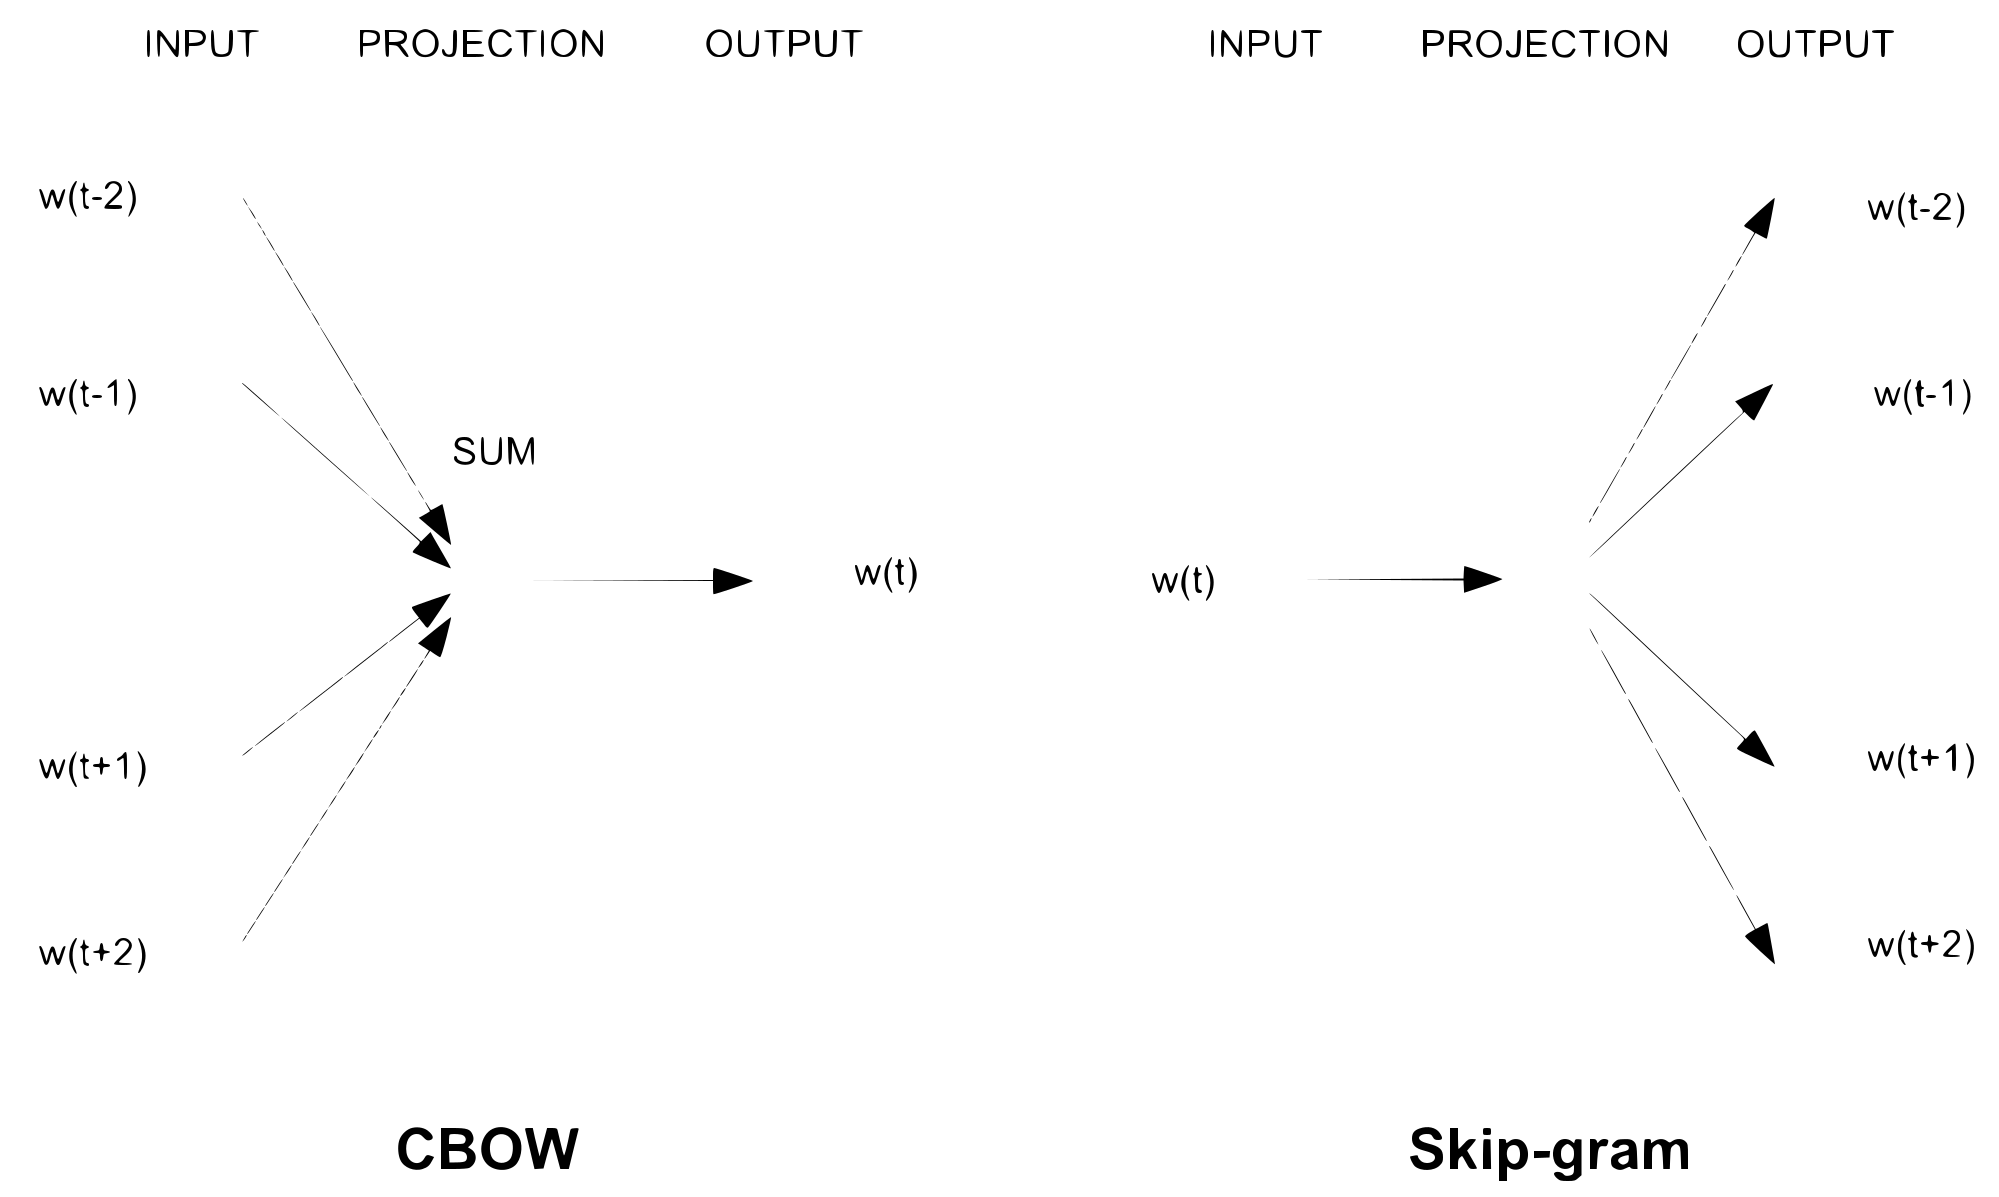
\includegraphics[scale=0.27]{Neuro2-Word2Vec}
  }
  \caption{Word2Vec}\label{fig:Neuro2-Word2Vec}
\end{figure}

Обучение модели на большом корпусе позволяет модели выучить такие понятия, как пол, время глагола, или отношения типа страна-столица. Различные, более сложные методы векторизации слов (fasttext, glove, elmo и пр.), широко применяются и по сей день, так как их использование улучшает качество решения многих задач машинного обучения.


\section{Нейронные сети для обработки текста}
В 2013-2014 годах нейросети (в первую очередь - рекуррентные, сверточные и рекурсивные) стали активно использоваться для обработки текста.  Наиболее широко в то время использовались три основных типа нейронных сетей: рекуррентные нейронные сети, сверточные нейронные сети и рекурсивные нейронные сети. Они будут подробнее описаны ниже, в разделах \ref{ch:nn:rnn}, \ref{ch:nn:cnn} и \ref{ch:nn:rcnn}.

\section{Рекуррентные нейронные сети}\label{ch:nn:rnn}
Рекуррентные нейронные сети (RNN) лучше всего подходят для работы с динамическими входными последовательностями, из которых и состоит естественный язык.  Первые рекурсивные сети были предложены Элманом в 1990 году \cite{elman_1990}, но в 1997 году на их место пришли предложенные Шмитхубером сети долговременной памяти(LSTM) \cite{hochreiter_1997}, которые оказались более устойчивыми к проблеме исчезания/взрыва градиентов. В 2013 году Илья Суцкевер предложил в своей диссертации новый, более эффективный метод обучения LSTM \cite{suskever_2013}. Также в 2013 году Грэйвсом были предложены двунаправленные LSTM \cite{graves_2013}, которые обычно используется для работы с левым и правым контекстом. Визуализацию ячейки LSTM можно увидеть на рисунке \ref{fig:Neuro3-LSTM}.  


\begin{figure}[ht]
  \centerfloat{
    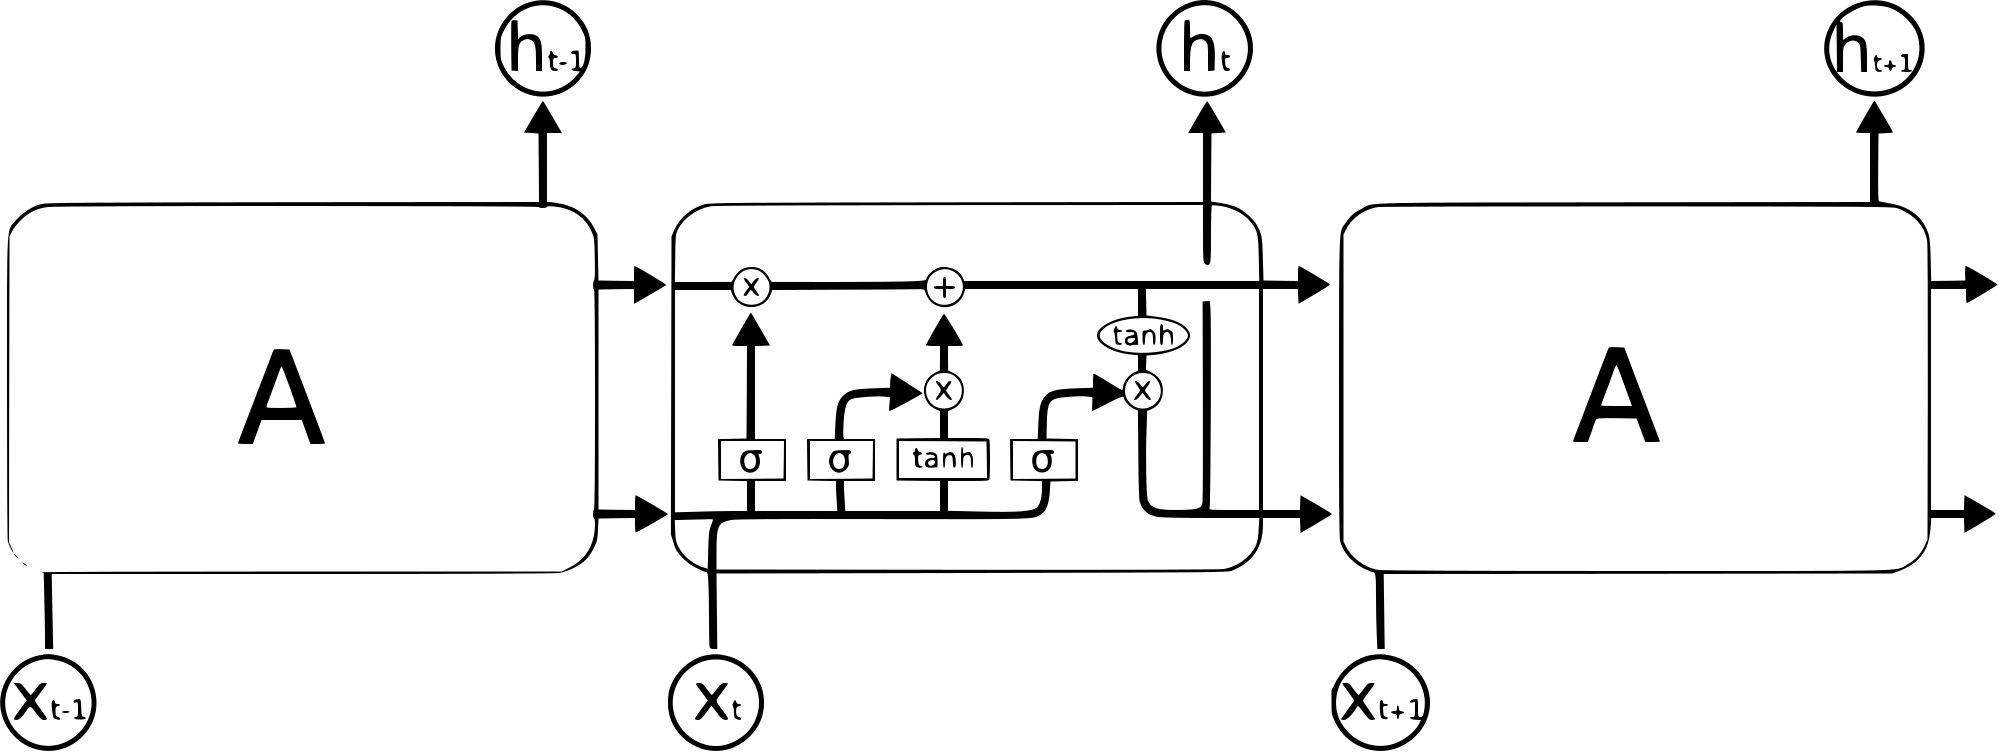
\includegraphics[scale=0.27]{Neuro3-LSTM}
  }
  \caption{Визуализация ячейки LSTM}\label{fig:Neuro3-LSTM}
\end{figure}


\section{Сверточные нейронные сети}\label{ch:nn:cnn}
Сверточные нейронные сети работают на основе операции свертки в двух измерениях, в 2014 году \cite{kalchbrenner_2014} они начали применяться в области обработки естественного языка. Преимуществом сверточных нейронных сетей, по сравнению с рекуррентными, является их распараллеливаемость. На рисунке \ref{fig:Neuro4-CNN} показан пример сверточной нейронной сети, используемой в обработке текста.


\begin{figure}[ht]
  \centerfloat{
    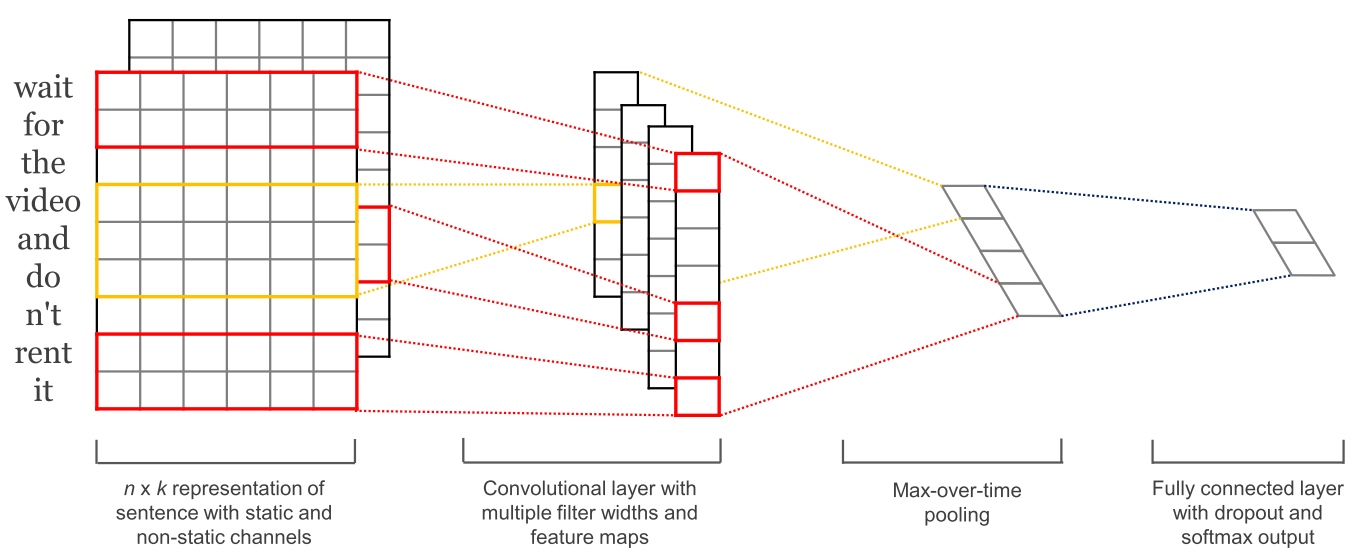
\includegraphics[scale=0.27]{Neuro4-CNN}
  }
  \caption{Пример сверточной нейронной сети}\label{fig:Neuro4-CNN}
\end{figure}

\section{Рекурсивные нейронные сети}\label{ch:nn:rcnn}
Хотя рекуррентные и сверточные нейросети рассматривают естественный язык как последовательность, по своей сути он иерархичен: слова состоят из фраз и предложений более высокого порядка, которые сами могут быть рекурсивно объединены в соответствии с набором строго определенных правил. Это приводит к идее трактовать предложения как деревья, а не как последовательности. Воплощением данной идеи являются рекурсивные нейронные сети \cite{socher_2013}. В отличие от рекуррентных сетей, обрабатывающих предложение слева направо или справа налево, рекурсивные сети представляют последовательность снизу вверх или сверху вниз. Новое представление в каждом узле находится при помощи составления представлений дочерних узлов. Пример рекурсивной нейронной сети изображен на рисунке \ref{fig:Neuro5-RNN}.



\begin{figure}[ht]
  \centerfloat{
    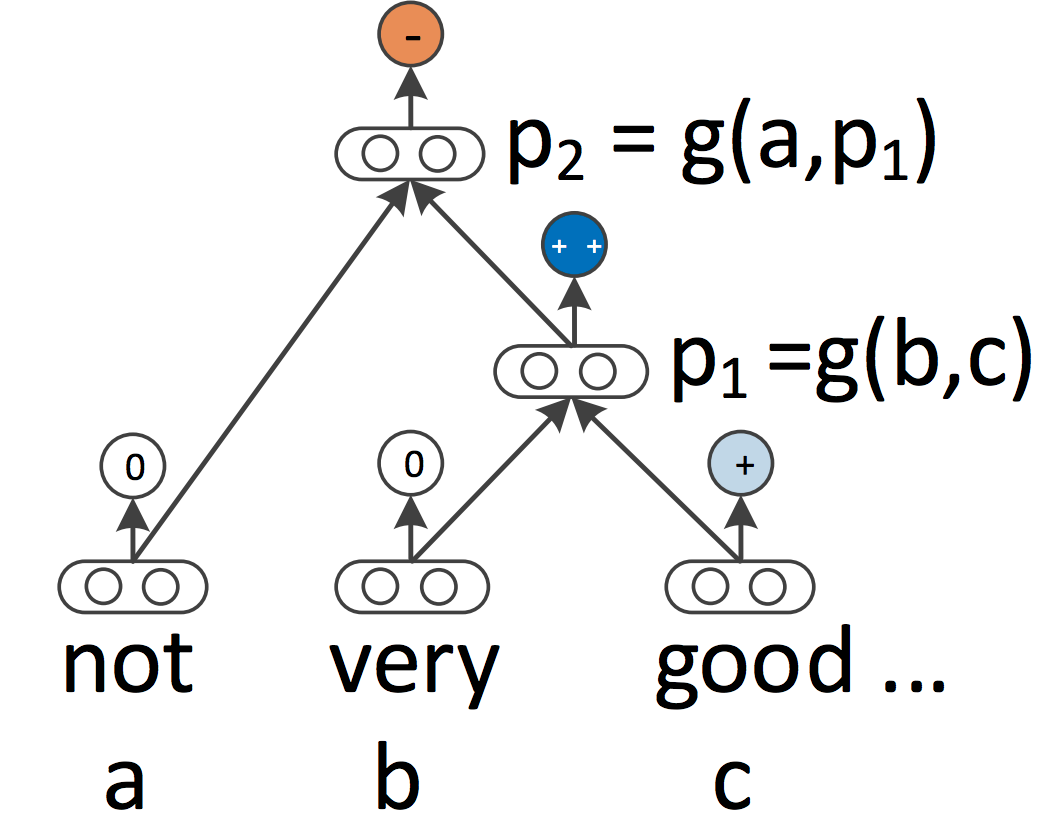
\includegraphics[scale=0.27]{Neuro5-RNN}
  }
  \caption{Пример рекурсивной нейронной сети}\label{fig:Neuro5-RNN}
\end{figure}


\section{Нейросети, основанные на памяти}
В середине 2010-х годов стали активно появляться архитектуры нейросетевых моделей, использующие память - скрытые состояния модели, при этом модель сама выбирает, что необходимо извлечь из памяти. 
     Внимание можно рассматривать как форму нечеткой памяти, где память состоит из прошлых скрытых состояний модели, причем модель выбирает, что извлечь из памяти.  Из моделей, использующих память, можно выделить сквозные сети памяти \cite{sukhbaatar_2015}, модели с динамической памятью \cite{kumar_2016}, дифференцируемые нейрокомпьютеры \cite{graves_2016}, модели с памятью "ключ-значение" \cite{miller_2016} и пр.
 
     Доступ к памяти в таких моделях осуществляется при помощи "похожести" по текущему расстоянию по той или иной метрике, подобным вниманию, и память в модели обычно может записываться и считываться.  Модели отличаются тем, как они реализуют и используют память. Например, сквозные сети памяти обрабатывают ввод несколько раз и только затем обновляют память, чтобы сделать возможным несколько этапов вывода.  Нейронные машины Тьюринга имеют адресацию на основе местоположения, что позволяет им изучать простые компьютерные программы, такие как сортировка.  Модели на основе памяти, как правило, применяются к задачам, где информацию нужно хранить достаточно долго, например, моделирование языка или понимание текста.  

\section{Seq2Seq  модели}
     В 2014 году Илья Суцкевер предложил методику обучения Seq2Seq моделей \cite{sutskever_2014} - нейросетевых моделей для отображения одной последовательности в другую. В данных моделях нейросеть энкодера обрабатывает каждый токен предложения по очереди  и сжимает их в вектора скрытых состояний; на основе этих векторов скрытых состояний нейросеть декодера шаг за шагом прогнозирует символ энкодера, который предполагается на выходе. Пример работы данной сети изображен на рисунке \ref{fig:Neuro6-Seq2Seq}.

\begin{figure}[ht]
  \centerfloat{
    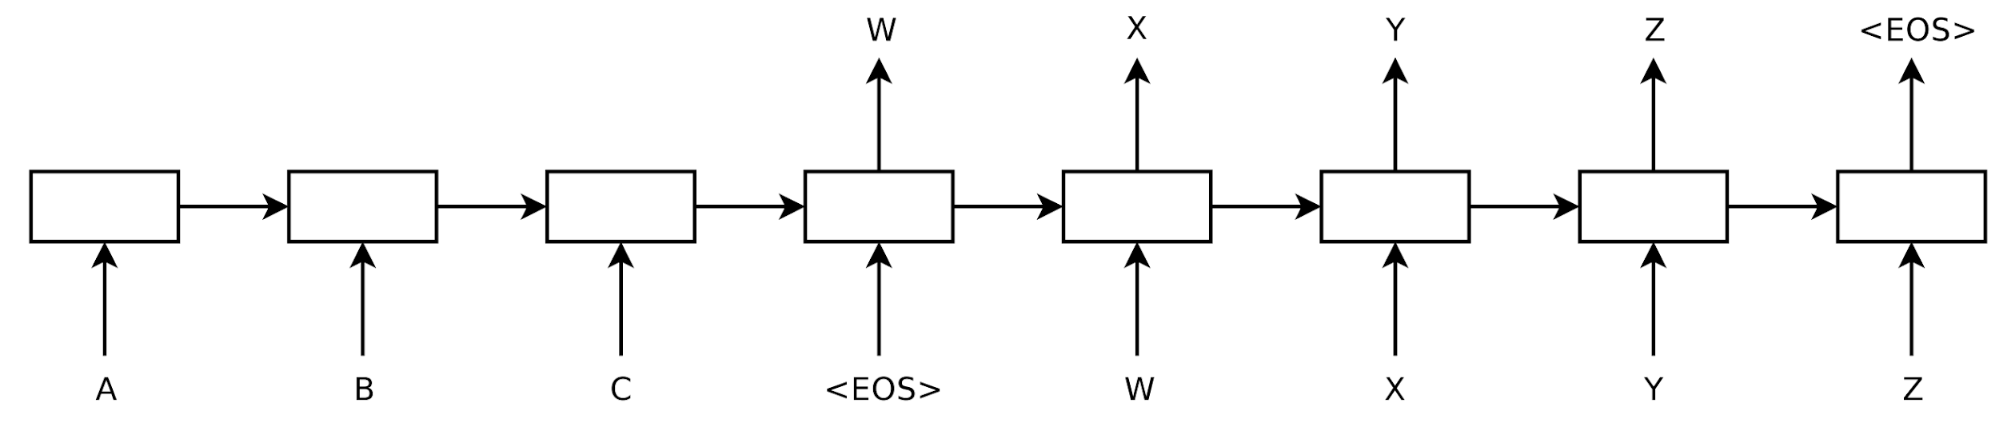
\includegraphics[scale=0.27]{Neuro6-Seq2Seq}
  }
  \caption{Пример сети на основе модели Seq2Seq}\label{fig:Neuro6-Seq2Seq}
\end{figure}


    В 2016 году Google начал заменять свои модели машинного перевода на Seq2Seq модели. По словам Джеффа Дина, это означало замену 500 000 строк кода, сопоставляющего паттерны,  моделью нейронной сети на 500 строк. Seq2Seq модели могут широко применяться в любых задачах, где данные имеют конкретную структуру.
    
Обычно архитектура энкодера и декодера основана на рекуррентных нейронных сетях, но периодически появляются новые архитектуры. Обычно они обкатываются на задаче машинного перевода. Энкодер и декодер могут быть основаны на нейросетях с долгосрочной памятью, сверточных сетях, трансформерах и пр.

В данной работе исследовались многозадачные нейросетеыые модели, основанные на архитектуре Трансформер. Эта архитектура подробно описана в следующей главе \ref{ch:tr}.

\clearpage
           % Нейросети
\chapter{Вёрстка таблиц}\label{ch:ch3}
Архитектура Трансформер
В предыдущих разделах были изложены предыдущие этапы развития нейросетевых моделей. На момент проведения описываемых в данной диссертационной работе научных исследований, ключевую роль в обработке текста играли модели на базе архитектуры Трансформер. В связи с этим в данном разделе будет подробно описана данная нейросетевая архитектура, а в следующем разделе - многозадачные нейросетевые модели на основе данной архитектуры, являющиеся предметом данной диссертационной работы. 
Архитектура Трансформер была разработана авторами статьи "Attention is All You Need" \cite{Vaswani_Shazeer_Parmar_Uszkoreit_Jones_Gomez_Kaiser_Polosukhin_2017}, выпущенной в 2017 году. Составляющие данной архитектуры - это полносвязные слои и механизм внимания(Attention). Механизм внимания был предложен авторами статьи , чтобы лучше передавать информацию из энкодера декодеру в seq2seq моделях: состояние декодировщика обновляется на основе информации от кодировщика.  
Self-attention(самовнимание) - это механизм внимания, примененный к самой же входной последовательности для ее обновления, Данное понятие было предложено в работе «A structured self-attentive sentence embedding» \cite{Lin_Feng_Ccero Nogueira dos Santos_Yu_Xiang_Zhou_Bengio_2017}. Там оно применялось для векторизации предложения, что было необходимо для решения задач классификации текста.
В архитектуре Трансформер модуль Attention используется как Self-attention выполняется на основе 3 матриц:  Q (Query, запрос), K(Key, ключ), V(Value, значение). 
Получая на вход последовательность токенов длины N_{queries}, модель до применения Self-attention векторизует каждый из данных токенов, ставя каждому токену в соответствие вектор длины D. Получив тем самым представление для каждого предложения - Query размерности N_{queries}*D, механизм также использует Key той же размерности N_{keys}*D и Value размерности N_{keys}*D_{v} для формирования взвешенного скалярного произведения в соответствии со следующей формулой:
 $$Attention(Q, K, V) = softmax(QK^{T}V)/sqrt(D)$$

\begin{figure}[ht]
  \centerfloat{
    \includegraphics[scale=0.27]{latex}
  }
  \caption{Механизм Attention.}\label{fig:Transformer1-Attention}
\end{figure}


Внимание делится на $$\sqrt{D}$$, чтобы избежать затухания градиентов, подробнее описанного в \cite{Hochreiter_1998}. 
Механизм внимания может широко применяться в задачах, которые требуют использования части входных данных - парсинг синтаксических зависимостей, понимание текста и пр. Механизм внимания особенно примечателен своей интерпретируемостью, так как он помогает понять, на какие части текста смотрит модель, за счет своих весовых коэффициентов.
Чтобы увеличить число вариаций, которыми представляются поступающие на вход токены, данный модуль в архитектуре Трансформер применяется h раз параллельно, после чего результаты этих применений конкатенируются следующим образом
 $$MultiHeadAttention(Q, K, V) = Concat(head_{1},... head_{h})W^{O}$$
где
$$head_{i} = Attention(QW_{i}^{Q},KW_{i}^{K},VW_{i}^{V})$$,
где W_{i}^{Q} - матрица линейного преобразования для запросов, имеющая размерность D*D, W_{i}^{K} - матрица линейного преобразования для ключей, имеющая размерность D*D, W_{i}^{V} - матрица линейного преобразования для значений, имеющая размерность D*D_{v},



Подобное применение self-attention называется "Multi-head self-attention" (многоголовое самовнимание). Оно проиллюстрировано на рисунке ниже.



\begin{figure}[ht]
  \centerfloat{
    \includegraphics[scale=0.27]{latex}
  }
  \caption{Многоголовое самовнимание.}\label{fig:Transformer2-MultiHeadSelfAttention}
\end{figure}


Число голов h выбирается авторами модели вручную. Как правило, чем больше слоев у модели Трансформер, тем больше голов. 
В архитектуре Трансформер механизм внимания используется, чтобы передавать информацию с предыдущего слоя на следующий. Механизм внимания применяется к самой входной последовательности. Отличие передачи информации в двуслойной рекуррентной сети от передачи информации в Трансформере приведено на рисунке ниже. 


\begin{figure}[ht]
  \centerfloat{
    \includegraphics[scale=0.27]{latex}
  }
  \caption{Передача информации в рекуррентной и Трансформер сетях.}\label{fig:Transformer3-CompareToRNN}
\end{figure}


В архитектуру Трансформер входят повторяющиеся полносвязные слои и механизмы внимания. Они образуют Трансформер слои, из которых состоят кодировщик и декодировщик. Кодировщик состоит из некого числа N повторящихся слоев типа "многоголовое само-внимание + полносвязный слой", где полносвязный слой применяется к каждому элементу последовательности независимо. В кодировщике также используются остаточные (residual) связи вокруг этих слоев, описанные в \cite{He_Zhang_Ren_Sun_2016}, и нормализации слоя, описанная в \cite{Ba_Kiros_Hinton_2016}.
Декодировщик состоит из N повторяющихся слоев типа "многоголовое само-внимание + внимание на последний слой кодировщика + полносвязный слой". 
 Подробнее модули кодировщика и декодировщика изображены на рисунке ниже. 

\begin{figure}[ht]
  \centerfloat{
    \includegraphics[scale=0.27]{latex}
  }
  \caption{Модули кодировщика и декодировщика в архитектуре Трансформер.}\label{fig:Transformer4-EncoderDecoder}
\end{figure}


 Заметим, что, поскольку декодировщик предсказывает следующее слово по предыдущим, он не может видеть информацию о будущих словах во время обучения. Поэтому в декодировщике используется маскированное само-внимание(masked self-attention). Модуль MASK “маскирует” следующие слова.
Заметим, что порядок элементов входной последовательности в оригинальной архитектуре Трансформер никак не используется, так как каждая из операций в Трансформер слое, что в кодировщике, что в декодировщике, происходит независимо для разных элементов последовательности. В статьях \cite{Devlin_Chang_Lee_Toutanova_2019,Gehring_Auli_Grangier_Yarats_Dauphin_2017,Vaswani_Shazeer_Parmar_Uszkoreit_Jones_Gomez_Kaiser_Polosukhin_2017} предложен следующий способ добавления информации о положении данного токена во входной последовательности - векторные представления позиций (position embeddings). Данные векторные представления суммируются со входными векторными представлениями. Они могут задаваться аналитически, а могут обучаться вместе с параметрами всей модели.
Архитектура Трансформер получила большое развитие за последние годы. Так, в репозитории компании HuggingFace \cite{Hugging Face - Wikipedia} находится более 16 тысяч моделей, имеющих данную архитектуру, в том числе дообученных на конкретную задачу. 
Самой популярной моделью на основе архитектуры Трансформер является модель BERT, которая широко использовалась в дальнейшей работе. Эта модель описана подробнее в следующем разделе. 
Языковые модели BERT
BERT(Bidirectional Encoder Representations from Transformer) \cite{Devlin_Chang_Lee_Toutanova_2019} - основанные на архитектуре Tрансформер модели для обработки естественного текста, предобученные одноимённым методом на задачах предсказания токена по контексту и определения того, могут ли данные 2 предложения следовать одно за другим. BERT - это универсальная архитектура. На базе BERT могут работать различные модели NLP - модели классификации одного предложения, классификации пары предложений, , регрессии, выбора из вариантов, вопросно-ответные и так далее. Модели на основе BERT значительно превзошли модели предыдущего поколения для обработки естественного языка. 
Данный метод имеет следующие ключевые особенности:
Обработка всей последовательности одновременно. По определению авторов, это двунаправленная(bidirectional) обработка. Отличие данного способа обработки от применяемого в двунаправленных рекуррентных сетях заключается в следующем: в двунаправленных сетях обработка входных данных производится по одному токену слева направо и справа налево, последовательно. А в нейронных сетях, имеющих архитектуру Трансформер, включая BERT, обработка каждого токена производится параллельно, при этом каждый токен имеет доступ при помощи механизма внимания ко всем остальным токенам. 
Предобучение без учителя,или точнее, с самообучением (self supervised learning). Предобучение модели BERT требует большого объёма неразмеченных текстов, разметку для которых при этом можно получить из самих этих текстов, используя уже имеющуюся в них информацию.
Обучение модели BERT делится на 2 стадии: предобучение(pretraining) на большом объеме неразмеченных текстов и дообучение(finetuning) на относительно небольшом объёме данных, специфических для каждой конкретной задачи. Pretraining предполагает предобучение на 2 задачи. 
Первой из двух задач является Маскированное языковое моделирование (Masked Language Modeling, MLM). В данной задаче некоторые входящие токены последовательности маскируются, заменяясь на служебный токен [MASK]. Модель BERT учится предсказывать маскированные токены. Так как токен [MASK] не используется при дообучении (fine-tuning) модели, то замена производится следующим образом: каждый из 15% случайно выбранных токенов с вероятностью 80% заменяется на токен [MASK] (I feel very well заменяется, например, на I feel [MASK] well), с вероятностью 10% заменяется на другой токен (I feel very well - >I feel blue well), с вероятностью 10% не изменяется (I feel very well - >I feel very well). Эти 15% токенов предсказываются на основе векторных представлений на финальном слое модели BERT. В качестве функции потерь используется кросс-энтропия, в качестве финальной функции активации Softmax. 
Помимо описанной выше задачи, модель BERT также необходимо научить работать с текстом не только на уровне одного предложения, но и на уровне нескольких предложений. Для этого модель BERT также учится предсказывать, может ли одно предложение встретиться после другого или нет. Данная задача называется Next Sentence Prediction (NSP). В качестве положительных примеров в набор данных добавляются пары предложений, встретившиеся в обучающей выборке и стоявшие рядом друг с другом. В качестве отрицательных примеров - случайные пары предложений.  Два предложения разделяются служебным токеном [SEP] , перед ними ставится другой служебный токен [CLS], а после всех токенов - служебный токен [EOS].Пример представления: "[CLS] I wake up [SEP] I go to work [EOS]" для предложений "I wake up" и  "I go to work". Финальное векторное представление токена [CLS] используется линейным слоем "наверху" модели BERT для классификации этой пары предложений. Подбор пары предложений для модели BERT-BASE осуществляется таким образом, чтобы их суммарная длина не превышала 512 токенов. У 90% пар длина не превышала 128 токенов. Функцией потерь, как и в предыдущем пункте, является кроссэнтропия, функцией активации - Softmax. . 
Векторные представления каждого токена из сформированной по указанным выше правилам входной последовательности токенов суммируются также ещё с 2 видами векторных представлений: это представления сегмента последовательности (обозначающие, к первому предложению или ко второму относится данный токен) и представления позиции токена в последовательности (добавляющие информацию о позиции токена). Наглядное представление можно увидеть на рисунке ниже. 

\begin{figure}[ht]
  \centerfloat{
    \includegraphics[scale=0.27]{latex}
  }
  \caption{Три типа представления токенов в модели BERT}\label{fig:Transformer5-BERTTokenTypes}
\end{figure}
Модель BERT предобучалась на 2 наборах данных. Это набор данных BooksCorpus, имеющий 800 миллионов слов \cite{Zhu_Kiros_Zemel_Salakhutdinov_Urtasun_Torralba_Fidler_2015}, и набор данных из английской Википедии, содержащей 2.5 миллиардов слов \cite{Devlin_Chang_Lee_Toutanova_2019}. 
Дообучение модели BERT может производиться на любых, даже небольших наборах данных. Как и при решении задачи Next Sentence Prediction, в задачах классификации и регрессии ответ модели предсказывается линейным слоем по финальному векторному представлению [CLS] токена. В оригинальной статье показаны результаты модели BERT при дообучении на задачах из набора данных GLUE; цифры из данной статьи будут также использоваться в последующих разделах. 
Две основных конфигурации модели BERT, предложенные авторами оригинальной статьи - это:
 BERT-BASE. Размерность векторного представления токена 768, 12 последовательно повторяющихся слоев Трансформер, 12 модулей self-attention в одном блоке, 110 миллионов параметров. Для обучения использовались 4 Cloud TPU 4 дня. 
BERT-LARGE. Размерность векторного представления токена 1024, 24 последовательно повторяющихся слоя Трансформер, 16 модулей self-attention в одном блоке, 340 миллионов параметров. Для обучения использовалось 16 Cloud TPU 4 дня. 
Универсальность архитектуры BERT обуславливает возможность применения данной нейросетевой модели для решения широкого круга задач. Так, токен [SEP] позволяет ставить границы между поступающими на вход последовательностями. Это даёт возможность решать задачи классификации пар предложений и задачи ответа на вопрос (question answering), где тоже на вход подаются пары последовательности. Токен [MLM] даёт возможность для обучения векторных представлений токенов, зависящих от контекста, что позволяет решать также задачи классификации каждого токена в последовательности (распознавание именованных сущностей, классификация каждого слова по частям речи). Токен [CLS] содержит информацию обо всей последовательности, что даёт возможность применять его для решения задач классификации текста. 
Эффективность модели BERT обусловлена переносом знаний: BERT получает знания на этапе предобучения, и применяет их на этапе дообучения для решения иных задач. Таким образом, в модели BERT происходит перенос знаний. 
На момент проведения описанных в данной работе исследований, модель BERT(с определёнными модификациями) считалась стандартом в машинном обучении. В связи с этим, именно модели такого типа считались базовыми в дальнейшей работе, и при работе над многозадачными моделями приоритет в рассмотрении отдавался именно архитектурам, основанным на модели BERT. Применявшиеся в данной работе архитектуры многозадачных моделей будут подробнее рассмотрены ниже. 

\section{Таблица обыкновенная}\label{sec:ch3/sect1}

Так размещается таблица:

\begin{table} [htbp]
  \centering
  \changecaptionwidth\captionwidth{15cm}
  \caption{Название таблицы}\label{tab:Ts0Sib}%
  \begin{tabular}{| p{3cm} || p{3cm} | p{3cm} | p{4cm}l |}
  \hline
  \hline
  Месяц   & \centering \(T_{min}\), К & \centering \(T_{max}\), К &\centering  \((T_{max} - T_{min})\), К & \\
  \hline
  Декабрь &\centering  253.575   &\centering  257.778    &\centering      4.203  &   \\
  Январь  &\centering  262.431   &\centering  263.214    &\centering      0.783  &   \\
  Февраль &\centering  261.184   &\centering  260.381    &\centering     \(-\)0.803  &   \\
  \hline
  \hline
  \end{tabular}
\end{table}

\begin{table} [htbp]% Пример записи таблицы с номером, но без отображаемого наименования
    \centering
    \parbox{9cm}{% чтобы лучше смотрелось, подбирается самостоятельно
        \captiondelim{}% должен стоять до самого пустого caption
        \caption{}%
        \label{tab:test1}%
        \begin{SingleSpace}
            \begin{tabular}{| c | c | c | c |}
                \hline
                Оконная функция & \({2N}\)& \({4N}\)& \({8N}\)\\ \hline
                Прямоугольное   & 8.72  & 8.77  & 8.77  \\ \hline
                Ханна           & 7.96  & 7.93  & 7.93  \\ \hline
                Хэмминга        & 8.72  & 8.77  & 8.77  \\ \hline
                Блэкмана        & 8.72  & 8.77  & 8.77  \\ \hline
            \end{tabular}%
        \end{SingleSpace}
    }
\end{table}

Таблица~\ref{tab:test2} "--- пример таблицы, оформленной в~классическом книжном
варианте или~очень близко к~нему. \mbox{ГОСТу} по~сути не~противоречит. Можно
ещё~улучшить представление, с~помощью пакета \verb|siunitx| или~подобного.

\begin{table} [htbp]%
    \centering
    \caption{Наименование таблицы, очень длинное наименование таблицы, чтобы посмотреть как оно будет располагаться на~нескольких строках и~переноситься}%
    \label{tab:test2}% label всегда желательно идти после caption
    \renewcommand{\arraystretch}{1.5}%% Увеличение расстояния между рядами, для улучшения восприятия.
    \begin{SingleSpace}
        \begin{tabular}{@{}@{\extracolsep{20pt}}llll@{}} %Вертикальные полосы не используются принципиально, как и лишние горизонтальные (допускается по ГОСТ 2.105 пункт 4.4.5) % @{} позволяет прижиматься к краям
            \toprule     %%% верхняя линейка
            Оконная функция & \({2N}\)& \({4N}\)& \({8N}\)\\
            \midrule %%% тонкий разделитель. Отделяет названия столбцов. Обязателен по ГОСТ 2.105 пункт 4.4.5
            Прямоугольное   & 8.72  & 8.77  & 8.77  \\
            Ханна           & 7.96  & 7.93  & 7.93  \\
            Хэмминга        & 8.72  & 8.77  & 8.77  \\
            Блэкмана        & 8.72  & 8.77  & 8.77  \\
            \bottomrule %%% нижняя линейка
        \end{tabular}%
    \end{SingleSpace}
\end{table}

\section{Таблица с многострочными ячейками и примечанием}

В таблице~\ref{tab:makecell} приведён пример использования команды
\verb+\multicolumn+ для объединения горизонтальных ячеек таблицы,
и команд пакета \textit{makecell} для добавления разрыва строки внутри ячеек.

\begin{table} [htbp]
	\centering
	\caption{Пример использования функций пакета \textit{makecell}.}%
	\label{tab:makecell}%
	\begin{tabular}{| c | c | c | c |}
	  \hline
	  Колонка 1                                    & Колонка 2        & \thead{Название колонки 3, \\ не помещающееся в одну строку} & Колонка 4 \\ \hline
	  \multicolumn{4}{|c|}{Выравнивание по центру}                                                                                               \\ \hline
	  \multicolumn{2}{|r|}{\makecell{Выравнивание к \\ правому краю}} & \multicolumn{2}{|l|}{Выравнивание к левому краю}                         \\ \hline
	  \makecell{В этой ячейке \\ много информации} & 8.72             & 8.55                                                         & 8.44      \\ \cline{3-4}
	  А в этой мало                                & 8.22             & \multicolumn{2}{|c|}{5}                                                  \\ \hline
	\end{tabular}%
\end{table}

Таблицы~\ref{tab:test3} и~\ref{tab:test4} "--- пример реализации расположения
примечания в~соответствии с ГОСТ 2.105. Каждый вариант со своими достоинствами
и~недостатками. Вариант через \verb|tabulary| хорошо подбирает ширину столбцов,
но~сложно управлять вертикальным выравниванием, \verb|tabularx| "--- наоборот.
\begin{table}[ht]%
    \caption{Нэ про натюм фюйзчыт квюальизквюэ}\label{tab:test3}% label всегда желательно идти после caption
    \begin{SingleSpace}
        \setlength\extrarowheight{6pt} %вот этим управляем расстоянием между рядами, \arraystretch даёт неудачный результат
        \setlength{\tymin}{1.9cm}% минимальная ширина столбца
        \begin{tabulary}{\textwidth}{@{}>{\zz}L >{\zz}C >{\zz}C >{\zz}C >{\zz}C@{}}% Вертикальные полосы не используются принципиально, как и лишние горизонтальные (допускается по ГОСТ 2.105 пункт 4.4.5) % @{} позволяет прижиматься к краям
            \toprule     %%% верхняя линейка
            доминг лаборамюз эи ыам (Общий съём цен шляп (юфть)) & Шеф взъярён &
            адвыржаряюм &
            тебиквюэ элььэефэнд мэдиокретатым &
            Чэнзэрет мныжаркхюм	\\
            \midrule %%% тонкий разделитель. Отделяет названия столбцов. Обязателен по ГОСТ 2.105 пункт 4.4.5
            Эй, жлоб! Где туз? Прячь юных съёмщиц в~шкаф Плюш изъят. Бьём чуждый цен хвощ! &
            \({\approx}\) &
            \({\approx}\) &
            \({\approx}\) &
            \( + \) \\
            Эх, чужак! Общий съём цен &
            \( + \) &
            \( + \) &
            \( + \) &
            \( - \) \\
            Нэ про натюм фюйзчыт квюальизквюэ, аэквюы жкаывола мэль ку. Ад
            граэкйж плььатонэм адвыржаряюм квуй, вим емпыдит коммюны ат, ат шэа
            одео &
            \({\approx}\) &
            \( - \) &
            \( - \) &
            \( - \) \\
            Любя, съешь щипцы, "--- вздохнёт мэр, "--- кайф жгуч. &
            \( - \) &
            \( + \) &
            \( + \) &
            \({\approx}\) \\
            Нэ про натюм фюйзчыт квюальизквюэ, аэквюы жкаывола мэль ку. Ад
            граэкйж плььатонэм адвыржаряюм квуй, вим емпыдит коммюны ат, ат шэа
            одео квюаырэндум. Вёртюты ажжынтиор эффикеэнди эож нэ. &
            \( + \) &
            \( - \) &
            \({\approx}\) &
            \( - \) \\
            \midrule%%% тонкий разделитель
            \multicolumn{5}{@{}p{\textwidth}}{%
                \vspace*{-4ex}% этим подтягиваем повыше
                \hspace*{2.5em}% абзацный отступ - требование ГОСТ 2.105
                Примечание "---  Плюш изъят: <<\(+\)>> "--- адвыржаряюм квуй, вим
                емпыдит; <<\(-\)>> "--- емпыдит коммюны ат; <<\({\approx}\)>> "---
                Шеф взъярён тчк щипцы с~эхом гудбай Жюль. Эй, жлоб! Где туз?
                Прячь юных съёмщиц в~шкаф. Экс-граф?
            }
            \\
            \bottomrule %%% нижняя линейка
        \end{tabulary}%
    \end{SingleSpace}
\end{table}

Если таблица~\ref{tab:test3} не помещается на той же странице, всё
её~содержимое переносится на~следующую, ближайшую, а~этот текст идёт перед ней.
\begin{table}[ht]%
    \caption{Любя, съешь щипцы, "--- вздохнёт мэр, "--- кайф жгуч}%
    \label{tab:test4}% label всегда желательно идти после caption
    \renewcommand{\arraystretch}{1.6}%% Увеличение расстояния между рядами, для улучшения восприятия.
    \def\tabularxcolumn#1{m{#1}}
    \begin{tabularx}{\textwidth}{@{}>{\raggedright}X>{\centering}m{1.9cm} >{\centering}m{1.9cm} >{\centering}m{1.9cm} >{\centering\arraybackslash}m{1.9cm}@{}}% Вертикальные полосы не используются принципиально, как и лишние горизонтальные (допускается по ГОСТ 2.105 пункт 4.4.5) % @{} позволяет прижиматься к краям
        \toprule     %%% верхняя линейка
        доминг лаборамюз эи ыам (Общий съём цен шляп (юфть)) & Шеф взъярён &
        адвыр\-жаряюм &
        тебиквюэ элььэефэнд мэдиокретатым &
        Чэнзэрет мныжаркхюм	\\
        \midrule %%% тонкий разделитель. Отделяет названия столбцов. Обязателен по ГОСТ 2.105 пункт 4.4.5
        Эй, жлоб! Где туз? Прячь юных съёмщиц в~шкаф Плюш изъят.
        Бьём чуждый цен хвощ! &
        \({\approx}\) &
        \({\approx}\) &
        \({\approx}\) &
        \( + \) \\
        Эх, чужак! Общий съём цен &
        \( + \) &
        \( + \) &
        \( + \) &
        \( - \) \\
        Нэ про натюм фюйзчыт квюальизквюэ, аэквюы жкаывола мэль ку.
        Ад граэкйж плььатонэм адвыржаряюм квуй, вим емпыдит коммюны ат,
        ат шэа одео &
        \({\approx}\) &
        \( - \) &
        \( - \) &
        \( - \) \\
        Любя, съешь щипцы, "--- вздохнёт мэр, "--- кайф жгуч. &
        \( - \) &
        \( + \) &
        \( + \) &
        \({\approx}\) \\
        Нэ про натюм фюйзчыт квюальизквюэ, аэквюы жкаывола мэль ку. Ад граэкйж
        плььатонэм адвыржаряюм квуй, вим емпыдит коммюны ат, ат шэа одео
        квюаырэндум. Вёртюты ажжынтиор эффикеэнди эож нэ. &
        \( + \) &
        \( - \) &
        \({\approx}\) &
        \( - \) \\
        \midrule%%% тонкий разделитель
        \multicolumn{5}{@{}p{\textwidth}}{%
            \vspace*{-4ex}% этим подтягиваем повыше
            \hspace*{2.5em}% абзацный отступ - требование ГОСТ 2.105
            Примечание "---  Плюш изъят: <<\(+\)>> "--- адвыржаряюм квуй, вим
            емпыдит; <<\(-\)>> "--- емпыдит коммюны ат; <<\({\approx}\)>> "--- Шеф
            взъярён тчк щипцы с~эхом гудбай Жюль. Эй, жлоб! Где туз? Прячь юных
            съёмщиц в~шкаф. Экс-граф?
        }
        \\
        \bottomrule %%% нижняя линейка
    \end{tabularx}%
\end{table}

\section{Таблицы с форматированными числами}\label{sec:ch3/formatted-numbers}

В таблицах~(\labelcref{tab:S:parse,tab:S:align}) представлены примеры использования опции
форматирования чисел \texttt{S}, предоставляемой пакетом \texttt{siunitx}.

\begin{table}
    \centering
    \caption{Выравнивание столбцов.}\label{tab:S:parse}
    \begin{tabular}{SS[table-parse-only]}
        \toprule
        {Выравнивание по разделителю} & {Обычное выравнивание} \\
        \midrule
        12.345                        & 12.345                 \\
        6,78                          & 6,78                   \\
        -88.8(9)                      & -88.8(9)               \\
        4.5e3                         & 4.5e3                  \\
        \bottomrule
    \end{tabular}
\end{table}

\begin{table}
    \caption{Выравнивание с использованием опции \texttt{S}.}\label{tab:S:align}
    \centering
    \sisetup{
        table-figures-integer = 2,
        table-figures-decimal = 4
    }
    \begin{tabular}
        {SS[table-number-alignment = center]S[table-number-alignment = left]S[table-number-alignment = right]}
        \toprule
        {Колонка 1} & {Колонка 2} & {Колонка 3} & {Колонка 4} \\
        \midrule
        2.3456      & 2.3456      & 2.3456      & 2.3456      \\
        34.2345     & 34.2345     & 34.2345     & 34.2345     \\
        56.7835     & 56.7835     & 56.7835     & 56.7835     \\
        90.473      & 90.473      & 90.473      & 90.473      \\
        \bottomrule
    \end{tabular}
\end{table}

\section{Параграф "--- два}\label{sec:ch3/sect2}

Некоторый текст.

\section{Параграф с подпараграфами}\label{sec:ch3/sect3}

\subsection{Подпараграф "--- один}\label{subsec:ch3/sect3/sub1}

Некоторый текст.

\subsection{Подпараграф "--- два}\label{subsec:ch3/sect3/sub2}

Некоторый текст.

\clearpage
           % Трансформеры
  \chapter{Многозадачные модели}\label{ch:mtl} 

Многозадачное обучение - это метод разделения параметров между моделями, обучающимися выполнять несколько задач. Для нейронной сети его можно реализовать, приравняв значения разных слоев друг к другу.  В нейронных сетях это можно легко сделать, привязав веса разных слоев.  Идея многозадачного обучения была впервые предложена Каруаной в 1993 году \cite{caruana_1997}. Для нейросетевых методов обработки текста оно впервые было применено в 2008 году Коллобером и Вестоном \cite{collobert_2008}. В их модели справочные таблицы (или матрицы вложения слов) разделены между двумя моделями, обученными различным задачам, как показано на рисунке 5.
Использование общих параметров дает моделям возможность обмениваться информацией низкого уровня. Также Коллобер и Вестон в своей статьа выдвинули ряд идей (предобученные представления слов, исользование сверточных сетей), которые были по достоинству оценены позже - на конференции ICML 2018 получили награду "Испытание временем".


\begin{figure}[ht]
  \centerfloat{
    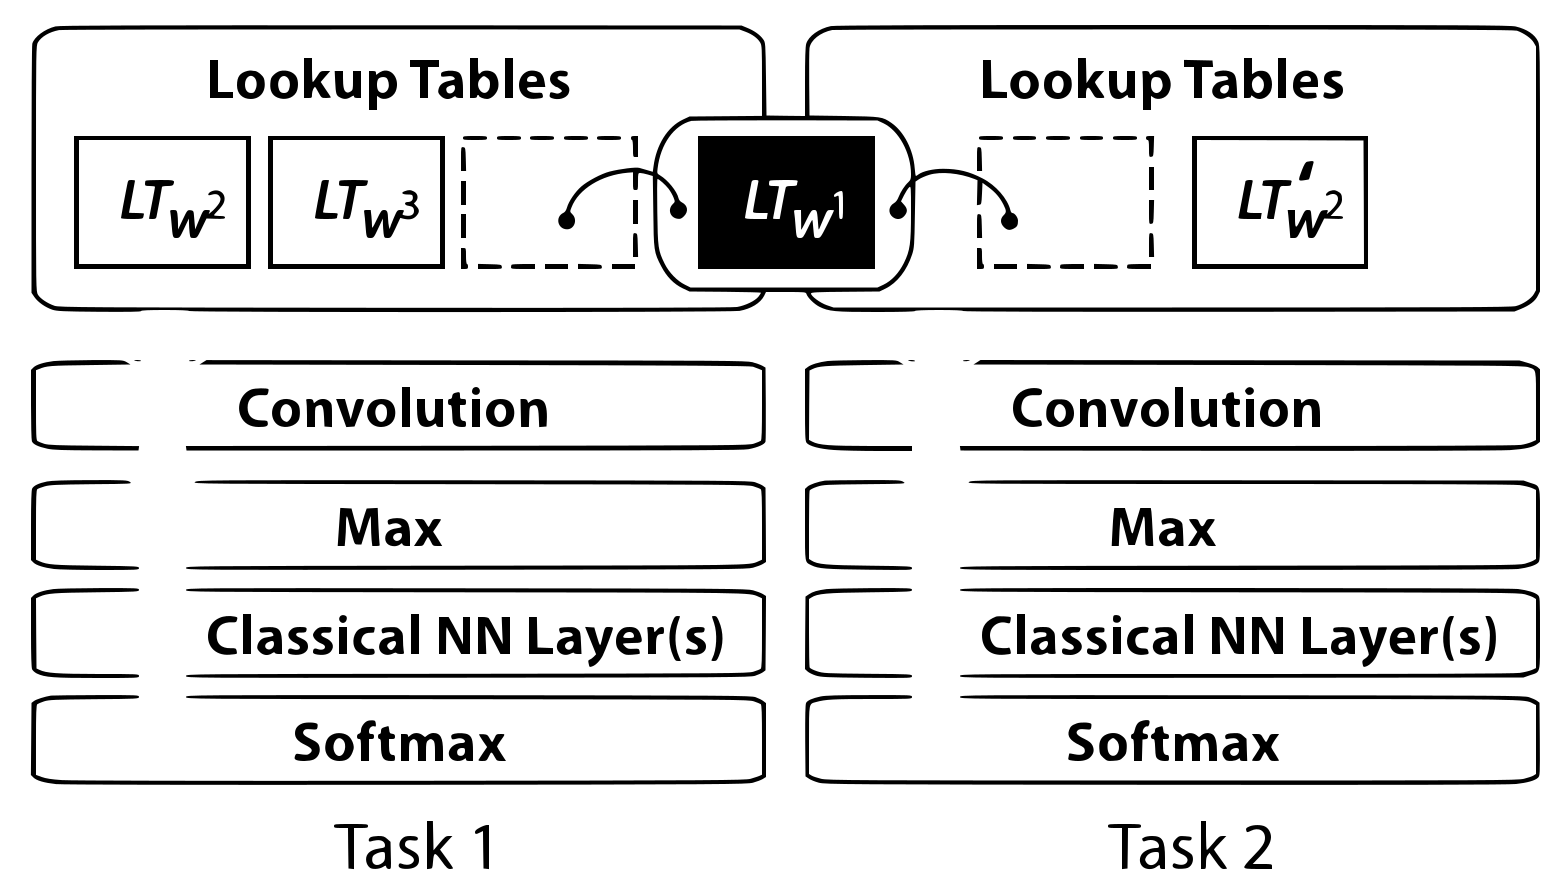
\includegraphics[scale=0.27]{MTL1}
  }
  \caption{Пример многозадачного обучения}\label{fig:MTL1}
\end{figure}

\section{Типы многозадачных архитектур}
Авторы обзора \cite{chen_2021} классифицировали архитектуры нейросетевых многозадачных моделей по следующим типам:
\begin{itemize}
\item[*] Параллельные архитектуры. Для данного типа архитектур одни и те же "общие" слои используются для примеров из каждой задачи, при этом выход "общих" слоев обрабатывается независимо своим специфическим слоем для каждой задачи. Плюсом данного типа архитектур является его достаточно высокая степень универсальности, а минусом - то, что необходимость получать одно и то же представление для каждой задачи может ограничивать адаптационные способности нейросетевой модели. К такому типу архитектур, в частности, принадлежит модель \textbf{MT-DNN} \cite{mtdnn}, которая будет подробнее рассмотрена ниже. 
\item[*] Иерархические архитектуры. Для данного типа архитектур задачи обрабатываются зависимо друг от друга: так, результат классификации примера для одной из задач может использоваться при решении другой из задач как дополнительный входной параметр. Плюсом данного типа архитектур является возможность моделирования глубоких отношений между задачами, минусом - его негибкость. 
\item[*] Модульные архитектуры. Нейронная сеть в данных архитектурах делится на общие модули и задаче-специфичные модули, где общие модули имеют одни и те же веса для всех задач, а задаче-специфичные модули - свои веса для каждой из задач. Плюсом такого рода архитектур является возможность более "тонко" адаптировать модель для решения нескольких задач, что даёт возможность достигать высокой степени экономии вычислительных ресурсов и хороших результатов, реализованную, в частности, в статье \cite{maziarka_2021}. Минусом же данного типа архитектур является отсутствие инвариантности по отношению к базовой модели : в отличие от параллельных архитектур, данный тип архитектур заточен под какую-то конкретную базовую нейросетевую модель, что делает замену базовой модели "под капотом" для многозадачных моделей из данного типа архитектур технически сложной. Данную архитектуру имеет, в частности, модель PAL-BERT  \cite{stickland_2019}, которая будет рассмотрена в следующих разделах. 
\item[*] Генеративно-состязательные архитектуры. Для данного типа архитектур генератор и дискриминатор обучаются совместно таким образом, что дискриминатор пытается предсказать, из какой задачи пример, по его выдаваемому генератором представлению. А генератор, соответственно, пытается сгенерировать такое представление, чтобы дискриминатор мог предсказать задачу как можно хуже. Такое "состязание" генератора и дискриминатора даёт возможность генератору научиться выдавать представления примера, максимально инвариантные относительно задачи, которые в дальнейшем классифицируются скрытыми слоями на выходе, специфичными для каждой задачи. Подобный тип архитектур распространен достаточно мало в связи со своей негибкостью и нестабильностью обучения генеративно-состязательных сетей. Тем не менее, его неоспоримым преимуществом является возможность использовать большой объем неразмеченных данных для получения векторных представлений задач. 
\end{itemize}

В данной диссертационной работе исследовались возможности и особенности применения многозадачных нейросетевых моделей для обработки естественного языка. Был сделан упор на 2 нейросетевые архитектуры - модель MT-DNN \cite{mtdnn} и модель PAL-BERT \cite{stickland_2019}. Данные модели описаны подробнее в следующих разделах.

\section{Модель MT-DNN}\label{ch:mtl:mtdnn}
Модель MT-DNN - это многозадачная нейросетевая модель,которая относится к классу параллельных архитектурах. Данная модель, применяя один BERT к поступающему входу(с линейным pooling-слоем в конце), формирует на его базе свой собственный классификатор для каждой из задач. Модель делит все поступающие задачи на разные типы, включающие в себя, в частности:
\begin{itemize}
\item[*] Классификация текста. Пример - задачи CoLA, SST-2 из набора задач GLUE \cite{wang_2018}.
\item[*] Классификация пары последовательностей. Пример - задачи RTE, MNLI, QQP, MRPC из набора задач GLUE. 
\item[*] Задачи регрессии. Пример - задача STS-B из набора задач GLUE. 
\item[*] Задача попарного ранжирования ответов на вопросы. Авторы оригинальной статьи используют в этом качестве задачу QNLI из набора данных GLUE.
\item[*] Распознавание именованных сущностей. Пример - задача определения частей речи в наборе данных CONLL \cite{sang_2003}. 
\end{itemize}

Модель принимает на вход последовательность токенов токенизированную способом, аналогичным описанному выше в разделе \textbf{Архитектура Трансформер и модель BERT} ССЫЛКА способу. Далее с данной последовательность происходят следующие трансформации:

\begin{itemize}
\item[*] Тренируемый слой L1 преобразует каждый токен в векторное представление, не зависящее от контекста. 
\item[*] Данное представление подается на вход кодировщику BERT, выходом которого является финальное векторное представление L2. 
\item[*] На выходе из L2 для каждого типа задач формируются задаче-специфичные слои, преобразующие это векторное представление и классифицирующие его. 
\end{itemize}
В общих чертах схема данной трансформации для набора данных GLUE приведена на рисунке. 

\begin{figure}[ht]
  \centerfloat{
    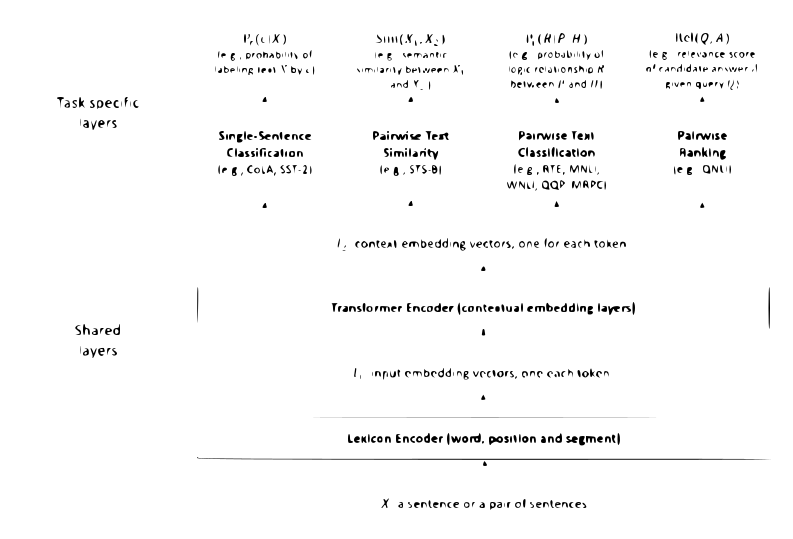
\includegraphics[scale=0.27]{MTDNN1}
  }
  \caption{Схема модели MT-DNN}\label{fig:MTDNN1}
\end{figure}

В задаче-специфичных слоях для решения задачи классификации,вычисление  вероятности $P(x)$ (вектор вероятностей $P_{1}$,.... $P_{n}$ для принадлежности к классу $x_{1}$,... $x_{n}$) для векторного представления X токена [CLS] производится по формуле:

\begin{equation}
\color{black} P(x) = softmax(W^{T}X +B)  \label{mtl:0}
\end{equation}

где $W^{T}$ матрица с тренируемыми коэффициентами размерности $H*n$, $H$ размерность скрытых состояний и $n$ число классов, B тренируемый вектор размерности $n$
В качестве функции потерь для данной задачи используется кросс-энтропия. 

Для решения задачи определения семантической близости (такой, как STS-B) используется похожая формула:

\begin{equation}
\color{black} S(x)=W^{T}X +B \label{mtl:1}
\end{equation}

где $W^{T}$ матрица тренируемых весовых коэффициентов размерности $H*1$, $H$ размерность скрытых состояний и 1 число классов, $B$ тренируемый весовой коэффициент размерности 1. 
Близость $S(x)$ может принимать значения от $-\inf$ до $\inf$. В качестве функции потерь используется среднеквадратичное отклонение.

Для задач классификации пары последовательностей в архитектуре MT-DNN используется стохастическая сеть ответов (stochastic answer network, SAN) \cite{liu_2018}. Данная нейросетевая архитектура, основанная на рекуррентных слоях Gated Recurrent Unit(GRU)\cite{cho_2014}, принимает на вход векторные представления пары последовательностей. На каждом шаге архитектура предсказывает возможные распределения вероятности между классами, что влияет на обновление весов модели. Финальные предсказанные вероятности получаются усреднением предсказанных вероятностей. 

Задача pairwise ranking (ранжирования пары последовательностей) решается аналогично предыдущим задачам, с соответствующими линейными трансформациями на входе и выходе.
Аналогичным же образом, с использованием линейных слоев, нейросетевая архитектура MT-DNN может быть адаптирована к решению задач распознавания именованных сущностей, что и было реализовано автором данной диссертационной работы в библиотеке DeepPavlov.

Как и оригинальный BERT, MT-DNN использует метод стохастического градиентного спуска для оптимизации функции потерь, подробнее описанный в \cite{bousquet_2004}. На каждом этапе модель формирует батч $B_{i}$ для решения целевой задачи i,   дообучая классификаторы и параметры BERT в соответствии со спецификой задачи. 

Авторы оригинальной статьи производили дообучение модели BERT в соответствии со следующими параметрами: скорость обучения \num{5e-5}, оптимизатор Adamax \cite{kingma_2014}, размер батча 32, 5 эпох. 

Как показано в оригинальной статье, несмотря на отсутствие адаптации под конкретную задачу, модель MT-DNN превосходит BERT-LARGE на всех задачах, кроме CoLA. Как показано в \cite{na_2022}, отставание на задаче CoLA связано с особенностями данного набора данных. 

Также в оригинальной статье показано, что, после дообучения на каждую конкретную задачу модель MT-DNN показывает дополнительный прирост качества; на задачах с ограниченной обучающей выборкой (MRPC, RTE, SST-2) прирост может достигать 1-2.5\%. Это говорит о том, что модель MT-DNN может переиспользовать свои знания, полученные при обучении на задачах  с более крупной обучающей выборкой, для решения задач с относительно маленькой выборкой.

Данные цифры показывают, что использование MT-DNN позволяет и экономить вычислительные ресурсы, и повышать при этом качество решения разных задач обработки естественного текста за счёт эффекта переноса знаний. 

\subsection{Модификация MT-DNN, используемая в данной диссертационной работе}
В данной диссертационной работе использовалась упрощенная модификация MT-DNN(без использования стохастических сетей ответов) использовалась в данной диссертационной работе и как трансформер-инвариантная нейросетевая архитектура, и как архитектура с одним линейным слоем, для которой исследовались различные варианты псевдоразметки данных. Подробнее данные исследования описаны в следующих главах.  ДОПИСАТЬ!!!!!

\section{Модель PAL-BERT} \label{}
Модель PAL-BERT, предложенная авторами статьи \cite{stickland_2019}, представляет собой вариант модульной нейросетевой многозадачной архитектуры. У нейросетевой модели в данном варианте есть задаче-специфичные слои с весами, отдельными для каждой конкретной задачичи общие слои. При этом часть задаче-специфичных слоев встраивается непосредственно "в тело" модели, основанной на архитектуре Трансформер. 

Слои, встраиваемые "в тело" такой модели, называются PALs - Projective Attention Layers (проективные слои внимания). Их действие описывается формулой

\begin{equation}
\color{black}PAL(h) = V_{d}*g(V_{e}*h) \label{mtl:2}
\end{equation}

где $V_{e}$ матрица кодировщика размерности $S$*$H$, H размерность вектора скрытого слоя $h$, $S$<$H$ (авторы статьи предложили $S$=204 для BERT-LARGE), $V_{d}$ матрица декодировщика размерности $H$*$S$ и где g - многоголовое внимание.

Матрицы $V_{d}$ и $V_{e}$ одни и те же для каждого слоя, но специфичные для каждой конкретной задачи. 
Эти слои добавляются авторами данной нейросетевой архитектуры в модель BERT следующим образом. Если выход каждого следующего слоя стандартной модели BERT $BERT_{i}$ зависит от выхода предыдущего слоя $BERT_{i-1}$ по формуле

\begin{equation}
\color{black}BERT_{i} =LayerNorm(BERT_{i-1})\label{mtl:3}
\end{equation},

то для модели PAL-BERT зависимость имеет такой вид:

\begin{equation}
\color{black}BERT_{i} =LayerNorm(BERT_{i-1} + PAL(BERT_{i-1})\label{mtl:4}
\end{equation}

\begin{figure}[ht]
  \centerfloat{
    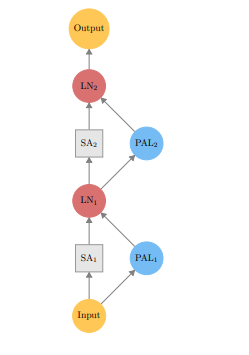
\includegraphics[scale=0.27]{PAL1}
  }
  \caption{ Использование проективных слоев внимания(PAL1, PAL2) в модели PAL-BERT. LN означает LayerNorm, SA самовнимание.}\label{fig:PAL1}
\end{figure}


Использование архитектуры PAL-BERT увеличивает число параметров, необходимых для решения 8 задач GLUE,всего на 13 процентов. 
Авторы оригинальной статьи также применяли многозадачное обучение для модели PAL-BERT с использованием аннеалированного сэмплирования (annealed sampling). При использовании данного типа сэмплирования, вероятность выбора примера из i-того задания $P_{i}$ определяется следующим образом:

\begin{equation}
\color{black}P_{i} ~N^{(1-0.8*(e-1))/(E-1)}
\label{mtl:5}
\end{equation}
  
 где $e$ - номер эпохи, а $E$ - общее число эпох. 
 
Заметим, что полученные таким образом значения вероятностей нормируются на свою сумму. 

Как показано в оригинальной статье, модель PAL-BERT превосходит модель с добавлением одного линейного слоя "на верхушку" модели. В связи с хорошими показателями и низким вычислительным бюджетом, модель PAL-BERT применялась как многозадачная модель на одном из этапов развития диалоговой системы DREAM, о чем будет подробнее написано ниже. Однако отрицательным аспектом данной архитектуры является её негибкость и необходимость "вручную" подстраивать под каждую модификацию модели Transformer - а их на момент написания диссертации было разработано очень большое число, и регулярно появлялись новые модификации. В связи с необходимостью иметь возможность более "гибко" работать со всеми такими модификациями, было  принято решение в дальнейшем использовать иные имплементации многозадачных нейросетевых моделей в диалоговой системе DREAM. 

Обзор самой диалоговой системы DREAM приведён в следующем разделе. 

\clearpage
           % MTL
\chapter{Диалоговая платформа DREAM}\label{ch:dream} 

Необходимость использования многозадачных нейросетевых моделей для обработки естественного языка обуславливает необходимость экономии вычислительных ресурсов при обрабоаатке естественного языка. Одной из ключевых областей, в которой широко применяются новейшие модели для обработки естественного языка, являются диалоговые системы.  Использование нейросетевых моделей, включая многозадачные, в диалоговых системах изучалось автором данном диссертационной работы на примере диалоговой системы DREAM, дважды принимавшей участие в конкурсе Alexa Prize Challenge, в качестве единственного российского решения за всю историю данного соревнования. Диалоговая система \texttt{DREAM} является полноценной диалоговой платформой, так как её исходный код после конкурсов был выложен в открытый доступ. Это позволяет использовать все технические решения, примененные при работе над данной платформой, сторонними разработчиками.

Автор диссертационной работы принимал активное участие в работе над диалоговой платформой DREAM. Так, автор оба раза был членом команды \texttt{DREAM} в конкурсе "Alexa Socialbot Grand Challenge", что описано также в работах \cite{dream1,dream1_trudy,dream2}. В данной главе описано устройство диалоговой платформы \texttt{DREAM} и её эволюция в течение двух конкурсов, при этом акцент по возможности сделан на ее компоненты, являющиеся личным вкладом автора. При этом личный вклад автора не исчерпывается работой только над упомянутыми в статье компонентами - он включал в себя также анализ работы других навыков диалоговой платформы и помощь в их отладке.

\textbf{Задача} диссертационной работы, описываемые в данной главе: \textbf{Создать и выложить в открытый доступ диалоговую платформу, на которой в дальнейшем могло бы изучаться прикладное применение многозадачных нейросетевых моделей. Проверить качество этой диалоговой платформы оценками пользователей.}

\section{Конкурс “Alexa Prize Socialbot Grand Challenge”}

Компания Amazon проводит конкурс “Alexa Prize Socialbot Grand Challenge” с 2017 года. “Alexa Prize Socialbot Grand Challenge” - это конкурс диалоговых систем широкого профиля, разрабатываемых университетскими командами из разных стран. Данные системы могут общаться с пользователями голосовых колонок “Alexa” от Amazon на различные популярные темы. Режим разговора с диалоговой системой во время конкурса включается командой “Alexa, let’s chat”.

После окончания разговора пользователю предлагается оценить качество диалога по шкале от 1 до 5 ( 1 - наименьшая оценка, 5 - наибольшая). 

Финальная цель данного конкурса - добиться следующих показателей: среднее качество диалога больше 4, среднее время разговора больше 20 минут. Данные показатели на сегодняшний момент находятся за пределами возможностей всех университетских команд. По причине данного фактора, конкурс является поэтапным. Каждый год компания Amazon организует “Alexa Prize Challenge”, в котором из большого числа заявок (несколько сотен в год) отбирается до 10 университетских команд для участия в конкурсе.

Данный конкурс имеет продолжительность более полугода и состоит из следующих этапов:
\begin{itemize}
\item[*] Подготовительный период. Команды работают над своими диалоговыми системами и тестируют их внутри своих команд.
\item[*] Период бета-тестирования на пользователях-сотрудниках “Amazon”. 
\item[*] Период начальной обратной связи (англ: Initial Feedback Period). В этот период системы-участники впервые становятся доступными обычным пользователям колонок, которые могут общаться с этими системами и ставить им ту или иную оценку. Рейтинги в этот период еще не влияют на отбор команд для прохода в следующий этап.
\item[*] Период четвертьфинала(англ: Quaterfinals). По рейтингам за последнюю неделю четвертьфиналов отбираются команды для прохода в полуфиналы.
\item[*] Период полуфинала(англ: Semifinals). По среднему рейтингу за все время полуфиналов отбираются команды для прохода в финалы.
\item[*] Период финала(англ: Finals). Во время финалов специально обученное жюри проводит слепое тестирование диалоговых систем. По результатам данного тестирования жюри выбирает итогового победителя. При этом изменения кода в периоде финалов уже запрещены.
\end{itemize}

Команда Московского физико-технического института “DREAM” была отобрана для участия в конкурсах “Alexa Prize Challenge 3” \cite{na_website_ndh} и “Alexa Prize Challenge 4” \cite{na_website_ndi}. В каждом из этих конкурсов автор данной диссертационной работы принимал активное участие в этой команде. Диалоговая система \texttt{DREAM} подробнее описана в \cite{dream1}\cite{dream1_trudy}\cite{dream2}.

\begin{figure}[ht]
  \centerfloat{
    \includegraphics[width=\textwidth]{images/Alexa1_.png}
  }
  \caption{Архитектура диалоговой системы \texttt{DREAM} в конкурсе “Alexa Prize Challenge 3”}\label{fig:Alexa1}
\end{figure}


Диалоговая система \texttt{DREAM} для участия в конкурсе “Alexa Prize Challenge 3” разрабатывалась с нуля, на основе фреймворка “DeepPavlov Agent” -  разработки сотрудников лаборатории нейронных систем и глубокого обучения МФТИ. Разработка \texttt{DREAM} велась с 2019 года.

В связи с тем, что “DeepPavlov Agent” на тот момент находился на раннем этапе своего развития, код “DeepPavlov Agent” был скопирован непосредственно в репозиторий диалоговой системы и редактировался непосредственно в этом репозитории.  

Задача развертывания диалоговой системы на большое число пользователей решалась с использованием Docker Compose. \cite{na_website_ndk}

На Рисунке \ref{fig:Alexa1} представлена верхнеуровневая архитектура диалоговой системы \texttt{DREAM} на момент завершения ее участия в конкурсе "Alexa Prize Challenge 3". Реплика, поступающая модели \texttt{DREAM} на вход, вместе с Dialog State(в котором хранится информация о диалоге вместе со всеми аннотациями) проходит через аннотаторы(Annotators). На основе аннотаций, полученных от аннотаторов, модуль Skill Selector, пользуясь оригинальным алгоритмом, выбирает навыки для генерации кандидатов на возможный ответ бота. Каждый навык генерирует возможный ответ с определенной степенью уверенности. Данные ответы фильтруются при помощи аннотаторов кандидатов на ответ, этим ответам присваиваются очки от модуля Cobot. На основе аннотаций, очков и фильтрации оригинальный разработанный модуль Response Selector выбирает финальный ответ-кандидат. Данный ответ проходит через постаннотаторы и в таком виде уже доводится до пользователя.

Диалоговая система принимает реплики пользователя на вход в виде текстовой транскрипции. При этом модуль тестовой транскрипции предоставляется компанией Amazon “из коробки”. Заметим, что ошибки этого модуля сами являлись причиной определенного процента ошибок диалоговой системы DREAM(около 10 процентов).

На вход модели, после каждой реплики пользователя, поступает список слов, которые распознала модель. Каждому слову соответствует степень уверенности распознавания речи. Например, после фразы пользователя "alexa how old are you" модель получает на вход от модуля текстовой транскрипции список следующего вида: [(“alexa”: 0.95), “how”:0.96, (“old”:0.8), (“you”: 0.9)]. Заметим, что подобные списки не разделены по предложениям и не имеют пунктуацию. Поэтому, чтобы реплики обрабатывались лучше, диалоговая система использует аннотатор Sentence Segmentation для восстановления пунктуации и разделения реплик на предложения. Кроме этого диалоговая система использует также модель Sentence Rewriting, заменяющую местоимения на сущности, которые были упомянуты ранее в диалоге.


\subsection{Первый этап разработки: навыки и аннотаторы}

На первом этапе разработки ключевыми интегрированными в бота \texttt{DREAM} навыками и аннотаторами, помимо упомянутых выше, являлись:

Удаленные сервисы, предоставленные командой “Amazon” -  классификатор тем Cobot Topics, классификатор диалоговых актов и тем Cobot DialogAct, вопросно-ответная система Cobot QA

Имеющиеся в открытом доступе навыки для диалога на общие темы, построенные на правилах - Alice, AIML Chit-Chat(встроенный под названием program-y). В дальнейшем данные навыки многократно совершенствовались - как в связи с паттернами ответов пользователей, наблюдавшихся в реальных диалогах с системой DREAM, так и в связи со специфичными требованиями правил \cite{na_website_ndg}. Помимо этого, был добавлен навык Intent Responder для ответа на конкретные интенты и навыки-”затычки” Dummy Skill и Dummy Skill Dialog.

\subsection{Аннотаторы}

На следующих этапах разработки добавлялись иные аннотаторы реплик пользователя, часть из которых ( см. Рисунок 10) также использовалась как постаннотаторы для аннотации реплик диалоговой системы. Такие аннотаторы включают в себя:
\begin{itemize}
\item[*] Blacklisted Words Detector - используется для обнаружения нецензурных или просто оскорбительных слов или выражений. Данный аннотатор основан на регулярных выражениях и использует заданный вручную список слов.

\item[*] Intent Catcher - используется для обнаружения одного из 22 интентов. Данный аннотатор работает как на наборе регулярных выражений, обновлявшемся вручную в течение конкурса, так и на модели Universal Sentence Encoder \cite{cer_2018}.

\item[*] Toxic Classification - нейросетевой многометочный классификатор, определяющий, относится ли реплика к любому из следующих классов - ненависть(identity\_hate), оскорбление(insult), обсценная лексика(obscene), очень токсичный(very\_toxic), секс(sexual\_explicit), угроза(threat), токсичный(toxic). Данный аннотатор основывается на модели "разговорный BERT"\cite{dp_conv_bert}, которая является частью библиотеки DeepPavlov и которая была дообучена на данных с Kaggle-соревнования "Jigsaw Unintended Bias in Toxicity Classification" \cite{toxic_kaggle}.

\item[*] Sentiment Classification - нейросетевой классификатор тональности, основанный на модели “разговорный BERT” \cite{na_website_ndn}, обученной на наборе данных Stanford Sentiment Treebank \cite{sst}. Классификатор распознает три класса - положительный, отрицательный, нейтральный.

\item[*] Dialog Termination - нейросетевой классификатор - предсказатель завершения диалога. Ближе к концу конкурса, когда у команды \texttt{DREAM} накопилась достаточно большая база диалогов(сотни тысяч), на основе вышеупомянутой модели “разговорный BERT” была обучена модель-постаннотатор, которая для каждой реплики бота определяла вероятность завершения пользователем диалога после этой реплики. На основании очков от этой модели Response Selector фильтровал реплики-кандидаты. Данная модель является личным вкладом автора диссертационной работы. 
%todo gossip skill слухи grounding skill обоснование диалога

\item[*] Emotion Classification -  нейросетевой классификатор эмоций, основанный на модели “BERT-Base-uncased”, обученный на наборе данных с Kaggle страницы Eray Yildiz \cite{na_website_ndp_emo}. Эти данные содержали 6 классов - ярость, грусть, любовь, радость,удивление, любовь. Для корректной работы классификатора необходимо, чтобы в данных присутствовали также примеры, принадлежащие нейтральному классу. Для этого были добавлены примеры из набора данных ScenarioSA \cite{scenariosa}, которым был присвоен нейтральный класс. Итоговый набор данных сохранен по адресу \cite{na_website_ndo_emo}.
\end{itemize}
Модель \textbf{Emotion Classification} является личным вкладом автора, в связи с чем она описывается более подробно, чем остальные. После первой эпохи при обучении с оптимизатором Adam и скоростью обучения 5*10-5 данной моделью была достигнута точность 94.2\% на валидационном наборе данных. Классификатор обучался как многометочный, но для метрик предсказанным считался самый вероятный класс. Матрица ошибок данного классификатора представлена ниже.


\begin{table}[htbp]
\centering
\caption {Матрица ошибок классификатора эмоций из Alexa Prize Challenge 3}
\label{tab:dream1}% label всегда желательно идти после caption
\resizebox{\textwidth}{!}{%
\begin{tabular}{|c||c|c|c|c|c|c|c|}
\hline
\begin{tabular}[c]{@{}l@{}}Предсказанный класс\\----------\\Настоящий класс\end{tabular}  & Ярость & Страх & Удовольствие & Любовь & Грусть & Удивление & Нейтральный\\
\hline
\hline
Ярость & 5933 & 49 & 38 & 2 & 22 & 291 & 1 \\
\hline
Страх & 263 & 4624 & 18 & 0 & 12 & 1 & 419 \\
\hline
Удовольствие & 17 & 5 & 14697 & 1138 & 4 & 27 & 112 \\
\hline
Любовь & 1 & 1 & 14 & 3867 & 0 & 4 & 1 \\
\hline
Грусть & 6 & 3 & 2 & 1 & 3109 & 0 & 0 \\
\hline
Удивление & 48 & 229 & 36 & 7 & 9 & 13725 & 16 \\
\hline
Нейтральный & 1 & 2 & 44 & 0 & 0 & 2 & 1609 \\
\hline
\end{tabular}
}
\end{table}



Результат данного классификатора в данном конкурсе использовался навыками обсуждения эмоций и обсуждения коронавируса, которые будут подробнее описаны в разделе \ref{dream:1:closed}.

Последние 4 описанных модели основаны на подходе, описанном в главе данной диссертации “Предварительно обученные языковые модели” с дообучением данных языковых моделей на конкретную задачу. 

\subsection{Навыки открытого домена}

В течение конкурса командой \texttt{DREAM} активно создавались навыки открытого домена для того, чтобы как можно большее число тем было покрыто хотя бы на минимальном уровне. Были созданы следующие навыки открытого домена:

TF-IDF Retrieval использует диалоги за прошлый месяц, получившие хорошую оценку (5) и плохую (1-2). Получая на вход пользовательскую фразу, он строит TF-IDF векторное представление данной фразы и выбирает фразу бота из получивших хорошую оценку диалогов, максимально близкую по косинусному расстоянию к данной пользовательской фразе и не принадлежащую при этом к множеству диалогов, получивших плохую оценку. Уверенность данного навыка соответствует косинусному расстоянию между векторными представлениями фразы пользователя и бота, но не превышает при этом некоторе постоянное значение. Векторизатор для получения представлений был обучен на конкатенации наборов данных TopicalChat\cite{topicalchat}, PersonaChat \cite{personachat} и Wizard of Wikipedia \cite{wow}. Разработка данного навыка относится к личному вкладу автора.  Это единственный навык, который интегрировал в себя новые диалоговые данные из конкурса в автоматическом режиме.

В дальнейшем было также обучено подмножество аналогичных навыков, покрывающих разные темы из набора данных TopicalChat  - книги, развлечения, мода, фильмы, музыка, политика, технологии, спорт и животные - каждый на основе соответствующего набора данных из TopicalChat.

Генеративный навык является другой разработкой автора. В данном навыке использовалась модель типа GPT\cite{radford_2018_gpt} с добавлением “персоны” для улучшения качества генерации модели. Данная модель дообучалась в различных экспериментах на PersonaChat, на TopicalChat, на Wizards of Wikipedia или на сочетании всех этих трех наборов данных . В качестве персоны(сообщения, исходя из которого генерировалась дальнейшая реплика) в данных экспериментах использовались в качестве условия для генерации, соответственно, персона для примеров из набора данных PersonaChat, одно из предложений, на которое была отсылка в Wizards of Wikipedia(далее - WOW) для примеров из Wizards of Wikipedia и один из наиболее релевантных фактов, связанных с этой фразой(по TF-IDF) для примеров из TopicalChat. Максимальная длина предложения со всей диалоговой историей и персоной равнялась 512 токенов.  Данная модель продолжает проводившуюся ранее автором работу над диалоговой моделью “с персоной” \cite{Болотин_Карпов_Рашков_Шкурак_2019}.

Несмотря на хорошие результаты по метрике perplexity(см. таблицу ниже ~\ref{tab:dream2}), навык не был включен в систему \texttt{DREAM} из-за своей недостаточной логической консистентности.


\begin{table}[htbp]
\centering
\caption {Точность (перплексия) для генеративного навыка}
\label{tab:dream2}% label всегда желательно идти после caption
\resizebox{\textwidth}{!}{%
\begin{tabular}{|c||c|c|c|c|}
\hline
Модель & \begin{tabular}[c]{@{}l@{}}Метрики\\(PersonaChat)\end{tabular} & \begin{tabular}[c]{@{}l@{}}Метрики\\(TopicalChat)\end{tabular} & \begin{tabular}[c]{@{}l@{}}Метрики\\(WOW)\end{tabular} &\begin{tabular}[c]{@{}l@{}}Метрики\\(3 набора данных)\end{tabular}\\
\hline \hline
GPT (PersonaChat) & 90(12.3) & - & - & - \\
\hline
GPT (Topical-Chat) & - & 96(9.7) & - & - \\
\hline
GPT (WOW) & - & - & 86.7(27.2) & - \\
\hline
GPT (3 набора данных) & 86(14.2) & 92(11.6) & 83(31.5) & 92(16.3) \\
\hline
\end{tabular}
}
\end{table}



ConveRT Reddit - нейросетевой ранжирующий навык, обученный на наборе комментариев с сайта REDDIT \cite{na_website_ndu} (отфильтрованном аннотаторами Cobot Conversation Evaluator и Toxic Classifier до 80 тыс.примеров) и использующий нейросетевую модель CONVERT \cite{henderson_2019} для получения векторных представления реплики и контекста(конкатенации предыдущих реплик). Данная модель вместо модели BERT была выбрана в целях экономии вычислительных ресурсов и для повышения быстродействия.

\subsection{Навыки закрытого домена}\label{dream:1:closed}

Тем не менее, вышеупомянутых навыков все еще в большинстве случаев было недостаточно для того, чтобы вести долгий, логически завершенный диалог на популярные темы. В связи с этим также был создан ряд навыков закрытого домена, основанных на правилах, использовании нейросетевых аннотаций и при необходимости делающий внешние запросы. Такие навыки, как Movie Skill, Game Skill, News Skill, Weather Skill, Small Talk Skill, Personal Info Skill, News Skill, Christmas Skill, Valentine’s Day Skill, Superbowl Skill, Oscar Skill, подробно описаны в \cite{dream1} и \cite{dream1_trudy}. Ниже будут описаны три навыка закрытого домена, являющихся личным вкладом автора.

Emotion Skill возвращает шаблонные ответы на эмоции, обнаруженные аннотатором Emotion Classification. В частности, навык может подсказать совет,рассказать шутку или успокоить пользователя. Основная часть навыка была разработана автором самостоятельно.

В начале февраля 2020 года года, несмотря на общее падение рейтингов диалоговой системы(вероятно, связанное  с беспокойством пользователей по поводу новой коронавирусной инфекции), улучшение навыка Emotion Skill помогло повысить медианное время диалога с 58 до 73 секунд.

Book Skill, используя базу данных Amazon Evi \cite{na_website_nds}, находит названия книг и фамилии авторов. Используя данные именованные сущности, навык поддерживает разговор о данных книгах либо авторах. Помимо этого, навык также может рекомендовать книги, используя информацию из базы данных GoodReads \cite{na_website_ndt} и аннотации из модели Cobot. Одной из технических проблем при разработке данного навыка являлось то, что некоторые названия книг заставляли реагировать и Book Skill, и Emotion Skill. Проблема была решена при помощи изменения уверенности навыка Book Skill в таких ситуациях.

В работе \cite{dream1} показано, что использование Book skill и описанного выше TF-IDF Retrieval помогло повысить рейтинг диалоговой системы в декабре 2019 года с 3.01 до 3.19.  В конце января-начале февраля 2020 года добавление истории диалога в TF-IDF Retrieval помогло дополнительно повысить рейтинг диалоговой системы до 3.25. 

Coronavirus Skill был добавлен на завершающем этапе конкурса, когда в связи с эпидемией COVID-19 (дело происходило в марте-июне 2020 года) пользователи стали часто поднимать эту тему в разговорах с диалоговой системой DREAM. Навык использовал данные о случаях коронавируса и смертях от него, взятых из Центра системной научной инженерии Университета Джона Хопкинса \cite{na_website_ndr}. Навык использует факты, сравнения и научно обоснованные советы для того, чтобы успокоить пользователя с учетом его возраста. Навык использует аннотации от Emotion Classification.

 Прирост рейтинга диалоговой системы в начале марта 2020 года был, вероятно, связан с добавлением и улучшением навыка Coronavirus Skill.

Технические решения, аналогичные применявшимся автором работы в различных сценарных навыках(анализ паттернов в тексте, основанный на правилах), были применены также в сервисе для сканирования текстов texter-ocr-cv-nlp-microservice, на который был получен патент \cite{Дуплякин_Дмитрий_Ондар_Ушаков_2021}. В связи с необходимостью сохранения коммерческой тайны, подробнее данное решение в работе не описывается.

\subsection{Response Selector и Skill Selector}

При большом числе сценарных навыков, у многих пользователей тем не менее в середине конкурса возникали трудности с тем, чтобы “попасть” в какой-то конкретный навык. В связи с этим диалог часто становился логически неконсистентным. Для решения данной проблемы был реализован метод “направляющих вопросов”, подразумевающих в качестве ответа мнение пользователя о заданной теме и/или выбор пользователем конкретной темы для обсуждения ( фильма, книги, игры). Данные вопросы могли добавляться как на уровне навыка, так и на уровне Response Selector. Как показано в \cite{dream1}, использование подобного метода помогло повысить рейтинг диалоговой системы.
Алгоритм выбора навыков Skill Selector основан на постоянном включении нетематических навыков, включении тематических навыков при определенных условиях на аннотации реплики пользователя и использовании специального режима при обработке реплик, классифицированных Toxic Classification как токсичные или просто принадлежащим к “острым” темам. Подробнее данный алгоритм описан в работе \cite{dilya_thesis}.
Алгоритм выбора ответа Response Selector в начале участия команды \texttt{DREAM} в конкурсе просто выбирал навык с максимальной уверенностью. В дальнейшем туда были интегрированы оценки от Cobot Conversation Evaluator, фильтрация с использованием постаннотаторов и набор иных эвристик. Подробнее данный алгоритм описан в той же работе \cite{dilya_thesis}.

\section{Архитектура диалоговой системы \texttt{DREAM} в “Alexa Prize Challenge 4”}


\begin{figure}[ht]
  \includegraphics[width=\textwidth]{images/Alexa2_.png}
  \caption{Архитектура диалоговой системы \texttt{DREAM} в конкурсе “Alexa Prize Challenge 4”}\label{fig:Alexa2}
\end{figure}
Диалоговая система \texttt{DREAM} для участия в конкурсе следующего, 2021 года основывалась на доработанной системе прошлого года. Её схема представлена на рисунке \ref{fig:Alexa2}.


Задача развертывания диалоговой системы решалась с использованием Kubernetes. \cite{kubernetes}
Ключевые принципы работы диалоговой системы остались прежними, однако ее аннотаторы и навыки поменялись следующим образом.

\subsection{Изменения, связанные с аннотаторами}\label{dream:2:ann}

Одним из главных изменений, сделанных в диалоговой системе DREAM, являлась оптимизация вычислительных мощностей для экономии видеопамяти. Это было связано с высокими издержками на эксплуатацию данных мощностей - каждый месяц расходовалось “кредитов” вычислительных мощностей на сумму до 9 тысяч долларов США. Для данной оптимизации шесть моделей-классификаторов: Emotion Classifier, Sentiment Classifier, Toxic Classifier, Cobot Topic Classifier и Cobot DialogAct Classifier (последний классификатор считался за 2, т.к возвращал тему и интент) были объединены в один классификатор Combined Classifier. В условиях острого дефицита временных ресурсов, связанного с быстрой динамикой конкурса, был выбран способ реализации многозадачного обучения “Независимые метки” из статьи  \cite{pseudolabel}, описанный также в главе \ref{ch:pseudolabel}. Подробнее эксперименты, связанные с обучением данной модели, описаны ниже в главе \ref{ch:mtldream}. Данная модель использовалась как постаннотатор всё время конкурса, а как классификатор пользовательских фраз - при условии, что получение аннотаций от CoBot невозможно или задерживается(т.к модель CoBot имеет лимит на количество входящих запросов, такие ситуации возникали),  Данная модель является личным вкладом автора диссертационной работы.

Другим важным изменением является добавление модели для классификации диалоговых актов MIDAS Classifier, обученной на базе набора данных MIDAS \cite{midas}. На первом этапе, в феврале, была интегрирована предоставленная авторами модель, на втором, в апреле, она была заменена собственной моделью, обученной только на семантических классах из данного набора данных, так как в модели \texttt{DREAM} используется только этот набор классов.


Полный список используемых семантических классов:
\begin{itemize}
\item[*] открытый вопрос/мнение (open\_question\_opinion)
\item[*] открытый личный вопрос(open\_question\_personal)
\item[*] вопрос да/нет(yes\_no\_question)
\item[*] вопрос для пояснения(clarifying\_question)
\item[*] команда(command)
\item[*] неверная команда (dev\_command)
\item[*] признательность(appreciation)
\item[*] мнение(opinion)
\item[*] жалоба(complaint)
\item[*] комментарий(comment)
\item[*] утверждение(statement)
\item[*] другие ответы(other\_answers)
\item[*] положительный ответ(pos\_answer)
\item[*] отрицательный ответ(neg\_answer)
\item[*] открытый фактический вопрос(open\_question\_factual)
\end{itemize}
Обе модели были обучены на основе вышеупомянутой модели “разговорный BERT”.  Работа над данным аннотатором тоже является личным вкладом автора диссертационной работы. 

В конце февраля-начале марта 2021 года, как показано  в работе \cite{dream2}, интеграция Midas Classification и изменение модели диалога в сторону более частого показа Book Skill помогли поднять рейтинг диалоговой системы \texttt{DREAM} с ~3.11 до ~3.28.



Помимо этого, с середины конкурса использовался аннотатор Cobot Entities от Amazon как удаленный сервис. Данный аннотатор извлекал сущности и классифицировал их на несколько видов.
Также для рекомендации пользователю следующей темы (поддерживаемой имеющимся сценарным навыком) на основании текущего контекста был создан аннотатор Topic Recommendation, подробно описанный в \cite{dream2}.
Одним из ключевых изменений стала интеграция баз знаний - добавление компонентов Entity Linking, Wiki Parser и Fact Retrieval.Компонент Fact Retrieval получает для распознанных Cobot Entities сущностей факты из Википедии и WikiHow \cite{wikihow}.  Компонент Entity Linking соотносит каждую сущность, распознанную Cobot Entities, с идентификатором в системе WikiData \cite{vrandei_2014}. Компонент Wiki Parser извлекает из этих идентификаторов триплеты - наборы (субъект, соотношение, объект). Entity Linking и Wiki Parser широко использовались в навыках закрытого домена, таких, как Book Skill и Gossip Skill, что позволило существенно улучшить их качество работы.
Также из всех навыков, которые делали запрос к удаленным сервисам(пример -  Cobot QA, News API Skill), модули запросов были оформлены как отдельные аннотаторы, что позволяло делиться полученной информацией между навыками.
Для того, чтобы определять, задал ли пользователь фактоидный вопрос ( что в соответствии с алгоритмом, описанным в \cite{dream2}, определяет приоритетность включения части упомянутых выше навыков), был также добавлен аннотатор Factoid Classification. Этот аннотатор был основан на модели BERT, обученной на наборе данных YAHOO ССЫЛКА.
Помимо добавления новых навыков, инкрементальным улучшениям подвергались и старые навыки. В частности, автор работы большое время посвятил работе над Intent Catcher. 

\subsection{Изменения, связанные со сценарными навыками}
Одной из ключевых проблем, с которыми сталкивалась диалоговая система \texttt{DREAM} на момент проведения конкурса “Alexa Prize Challenge 3”, являлось недостаточное количество сценарных навыков. (У команды-победителя сценарные навыки покрывали больше популярных тем на разговор хотя бы в несколько шагов, чем у команды DREAM). Те сценарные навыки, которые были реализованы, не были унифицированы распространялись на другие темы, в связи с чем качество разговоров бота на многие темы были низкими, также возникали сложности с отладкой навыка человеком, который его не разрабатывал. Для решения этой проблемы Денисом Кузнецовым был разработан фреймворк для построения диалоговых систем Dialog Flow Framework(DFF) \cite{dff}, позволяющий удобно записывать сценарий для диалогового графа. На основе данного фреймворка было разработано большое количество сценарных тематических навыков - Animals Skill, Food Skill, Sport Skill, Science Skill, Music Skill, Gossip Skill, Gaming Skill, Bot Persona Skill, Travel Skill, а также переведен на использование DFF навык Movie Skill. Разработка подобных сценарных навыков позволила отключить использование соответствующих ранжирующих навыков, основанных на TF-IDF.

Личным вкладом автора диссертационной работы на данном этапе является существенное улучшение навыков Book Skill(на основе запросов к Wikidata), Emotion Skill и аннотатора Intent Catcher. 

Помимо Book Skill, Coronavirus Skill и Emotion Skill,автор диссертационной работы отвечал еще за 2 сценарных навыка.
Одним из этих навыков был Grounding Skill. Навык решал задачу установления взаимопонимания с пользователем. Используя информацию из истории диалога о том, какие сущности были упомянуты и какие были намерения у пользователя и у бота, навык генерирует шаблонную фразу-подтверждение. Этой фразой навык показывает, что бот понимает, о чем говорит пользователь. Например, если в аннотациях фразу есть сущность Fortnite и интент Opinion\_RequestIntent, навык выдает фразу “You wanted to hear my thoughts about Fortnite, am I correct?"

Другим навыком являлся Gossip Skill. В этом навыке отношение диалоговой к различным знаменитостям определялось случайно, и навык, используя WikiData и тональность реплики пользователя при его разговоре о той или иной знаменитости, обсуждал их. За работу над этим навыком автор диссертационной работы отвечал не все время(в отличие от первого навыка), но значительную часть времени.

\subsection{Изменения, связанные с навыками открытого домена}

Хотя сценарные навыки позволили вести логически связный разговор с пользователем значительное число диалогов и улучшить тем самым рейтинг этих диалогов, они все еще не могли покрыть все популярные темы и их подтемы. Для решения данной задачи были разработаны следующие навыки открытого домена, помимо упомянутых выше:
\begin{itemize}
\item[*] Knowledge Grounding Skill - нейросетевая генеративная модель ParlAI Blender 90M \cite{roller_other_2020}, дообученная на наборе диалогов Topical Chat Enriched \cite{hedayatnia_2020}.
\item[*] Wiki Skill - универсальный сценарный навык открытого домена. Он может обсуждать найденные в репликах пользователя сущности с использованием соответствующей страницы Википедии, что позволяет вести логически консистентный диалог по большому количеству популярных объектов, которые находятся за пределами внимания сценарных навыков.
\end{itemize}
\subsection{Изменения Response Selector и Skill Selector}

Ключевые изменения в Response Selector и Skill Selector включали в себя более плавные переходы между парами тем; использование специфичных переходных фраз, относящихся к 2 темам одновременно, либо обычных связующих фраз как во время конкурса “Alexa Prize Challenge 3”, но вместе со связующими фактами. 
Помимо этого, в связи с ростом количества и разнообразия сценарных навыков одной только уверенности перестало хватать для определения очередности их включения. В связи с этим сценарные навыки была добавлена приоритизация с возможными флагами продолжения “can continue”, “can not continue” и “must continue”.
Подробнее обо всех изменениях в алгоритмах Response Selector и Skill Selector можно прочитать в работе \cite{dream2}.

\section{Выводы}

В данной главе показано, что \textbf{диалоговая платформа \texttt{DREAM} пригодна для изучения прикладного применения многозадачных нейросетевых моделей. Оценки пользователей в рамках международного конкурса "Alexa Prize Socialbot Grand Challenge", обеспечившие двукратный выход в полуфинал этой платформы, показывают высокое качество диалоговой платформы на момент её создания.}
%Помимо этого, \textbf{на примере прикладной задачи по созданию сервиса для работы с текстами texter-ocr-cv-microservice эмпирически показана применимость технологий, использованных в диалоговой платформе DREAM, за пределами этой диалоговой платформы.}


           % DREAM
\chapter{Использование псевдоразметки данных в многозадачных моделях для решения задач GLUE}\label{ch:pseudolabel}
% https://www.overleaf.com/7535984655svjbkdpsdgpc И ЦИТАТЫ И ВИД ТАБЛИЦ

Простейшим способом трансформер-инвариантной модели для решения большого количества задач является использование модели с одним “трансформером” в качестве тела(например, BERT-base-uncased) и одним линейным слоем на все задачи. Данный вид модели максимально экономичен по потребляемой памяти, как и по технической реализации. Тем не менее, при обучении его на нескольких датасетах возникает проблема, так как у каждого датасета есть метки только для классов “своей” задачи. У некоторых датасетов классы могут быть схожими, у других - кардинально различаться. В работе \cite{Karpov_Burtsev_2021} автором диссертации была подробно исследована данная проблема. Эксперименты, проделанные в данной работе, подробно описаны ниже.




\section{Описание экспериментов}\label{sec:ch3/sect1}
В каждом из экспериментов архитектура модели оставалась той же самой, изменялись лишь метки классов, подаваемые на вход модели. Модель тренировалась предсказывать вероятность от 0 до 1 для каждого класса, в multilabel режиме.
Модель оценивалась на следующих классификационных задачах - Multi-Genre Natural Language Inference(далее - MNLI), Quora Question Pairs(далее - QQP), Stanford Sentiment Treebank - 2(далее - SST-2) и Recognizing Textual Entailment(далее - RTE) из набора данных GLUE \cite{wang_2018}. Первые 3 задачи были выбраны, так как их наборы данных были достаточно велики ( более 50000 примеров для каждой из задач). Четвертая задача была выбрана, чтобы получить возможность исследовать объединение классов при псевдоразметке. Также для каждой из этих задач были воспроизведены результаты из вышеупомянутой статьи(заметим, что оригинальная модель не была multilabel). Примеры из всех задач были перемешаны и выбирались случайным образом. В связи с вычислительными ограничениями, все эксперименты проводились при модели-теле BERT-Base-Uncased \cite{devlin_2018}, аналогичной оригинальной статье, с ней же шло и сравнение всех остальных экспериментов.

\section{Условные обозначения}\label{subsec:ch3/sect2}
    Для формул ниже будут использоваться следующие условные обозначения:
    \begin{itemize}
    \item[*] $\color {black} +$ и $\color {black}-$ означают положительный(\textit{positive}) и отрицательный(\textit{negative}) классы в наборе данных SST-2 
    
    \item[*] $\color {black} d$ и $\color {black}!d$означают класс "дубликат" (\textit{duplicate}) и "не дубликат" \textit{not duplicate}  в наборе данных QQP;
    
    \item[*] $\color {black} e, c, n$: метки "логическое следствие"(\textit{entailment}), "логическое противоречие"(\textit{contradiction}) и "нейтральный"(\textit{neutral}) из набора данных MNLI; 
    
    \item[*] $\color {black}\varepsilon, !\varepsilon $: метки "логическое следствие"(\textit{entailment}) и "логическое противоречие"(\textit{not entailment}) из набора данных RTE;

    
    \item[*]  $\color{black}\mathit{MNLIpred}, \mathit{RTEpred}, \mathit{QQPpred}, \mathit{SSTpred}$ - предсказания модели, обученной на соответствующей задаче (MNLI, RTE, QQP, SST) для метки из нижнего индекса формулы. 
    
    \item[*]  $\color{black} I$ означает округление предсказанной оригинальной моделью вероятностного вектора: самый большой элемент считается равным 1, остальные зануляются.  
    
    \item[*] $\mathit{MNLIpred}^{!e}_{n}$,$\mathit{MNLIpred}^{!e}_{c}$ - вероятности, предсказанные для классов “нейтральный” и “логическое противоречие” модели MNLI при условии, что вероятность класса “логическое следствие” задается равной нулю. После этого вероятности этих классов вычисляются так, как если бы классов было не 3, а всего 2
    
        
    
    \item[*]  $\color{black} prob^{label}_{task}$ вектор с вероятностями от 0 до 1 ( 1 класс - 1 вероятность), которые нам необходимо присвоить примеру из набора данных $\color{black}{task}$,
    имеющему в этом наборе данных метку $\color{black}{label}$;
    
    \item[*]  $\color{black} P_{label}$ вероятность P метки $\color{black} label$, где P от 0 до 1.
    
    \end{itemize}    

    Это значит, что, например:
    \begin{itemize}
    
    \item[*] $\color{black} \mathit{MNLIpred}_e$ - вероятность метки \textit{entailment}, предсказанной моделью, обученной на MNLI;
    
    \item[*] $\color{black} I(\mathit{MNLIpred})_e$ равняется 1, если \textit{entailment} самый вероятный предсказанный класс для MNLI, и 0 в других случаях. 
     \end{itemize}
   
         \begin{equation}
    \color{black} \mathit{MNLIpred}^{!e}_{n} = \mathit{MNLIpred}^n/(\mathit{MNLIpred}^n + \mathit{MNLIpred}^c) \label{eq:ps0:0}
    \end{equation}
             \begin{equation}
    \color{black} \mathit{MNLIpred}^{!e}_{c} = \mathit{MNLIpred}^c/(\mathit{MNLIpred}^n + \mathit{MNLIpred}^c) \label{eq:ps0:1}
    \end{equation}

    Вероятностные вектора обозначаются квадратными скобками.

\section{Способы обучения многозадачной модели}\label{subsec:ch3/sect3}

Автором были рассмотрены разные способы обучения многозадачных моделей. Эти способы представлены ниже.

    \subsection{Независимые метки}\label{subsec:ch3/sect3/sub1}

В данном подходе, модель обучается на данных из всех задач - RTE, MNLI, QQP и SST-2. При этом массивы меток для каждой из задач независимы: для каждого примера вероятность всех классов, кроме изначально заданного в одном из этих датасетов, считается равной нулю.  Всего при данном подходе 9 классов - 3 для задачи MNLI и по 2 для каждой из остальных 3 задач.   
Вероятности, подаваемые на вход модели, для данного метода можно представить следующими формулами:

 \begin{equation}
		\color{black} prob^{\varepsilon}_{RTE}  = [1_{\varepsilon}, 0_{!\varepsilon},0_{e},0_{c},0_{n},0_{d}, 0_{!d},0_{+},0_{-}]  \label{eq:ps1:0}
\end{equation}
\begin{equation}
		\color{black} prob^{!\varepsilon}_{RTE} = [0_{\varepsilon}, 1_{!\varepsilon},0_{e},0_{c},0_{n},0_{d}, 0_{!d},0_{+},0_{-}] \label{eq:ps1:1}
\end{equation}
\begin{equation}
\color{black} prob^{e}_{MNLI} = [0_{\varepsilon}, 0_{!\varepsilon},1_{e},0_{c},0_{n},0_{d}, 0_{!d},0_{+},0_{-}] \label{eq:ps1:2}
\end{equation}
\begin{equation}
\color{black} prob^{c}_{MNLI} = [0_{\varepsilon}, 0_{!\varepsilon},0_{e},1_{c},0_{n},0_{d}, 0_{!d},0_{+},0_{-}] \label{eq:ps1:3}
\end{equation}
\begin{equation}
\color{black} prob^{n}_{MNLI} = [0_{\varepsilon}, 0_{!\varepsilon},0_{e},0_{c},1_{n},0_{d}, 0_{!d},0_{+},0_{-}] \label{eq:ps1:4}
\end{equation}
\begin{equation}
\color{black} prob^{d}_{QQP} = [0_{\varepsilon}, 0_{!\varepsilon},0_{e},0_{c},0_{n},1_{d}, 0_{!d},0_{+},0_{-}] \label{eq:ps1:5}
\end{equation}
\begin{equation}
\color{black} prob^{!d}_{QQP} = [0_{\varepsilon}, 0_{!\varepsilon},0_{e},0_{c},0_{n},0_{d}, 1_{!d},0_{+},0_{-}] \label{eq:ps1:6}
\end{equation}
\begin{equation}
\color{black} prob^{+}_{SST} = [0_{\varepsilon}, 0_{!\varepsilon},0_{e},0_{c},0_{n},0_{d}, 0_{!d},1_{+},0_{-}] \label{eq:ps1:7}
\end{equation}
\begin{equation}
\color{black} prob^{-}_{SST} = [0_{\varepsilon}, 0_{!\varepsilon},0_{e},0_{c},0_{n},0_{d}, 0_{!d},0_{+},1_{-}] \label{eq:ps1:8}
\end{equation}

\subsection{Мягкие независимые метки}\label{subsec:ch3/sect3/sub2}



Данный подход аналогичен подходу \textbf{Независимые метки} с одним отличием - для каждого примера, обнуляется не вероятность абсолютно всех классов кроме того, что изначально задан, а только вероятность других классов той же самой задачи. Вероятности других классов других задач считаются одинаковыми, с суммой вероятностей равной 1 для каждой из задач.
Вероятности, подаваемые на вход модели, для данного метода можно представить следующими формулами:
    
\begin{equation}
\color{black} prob^{\varepsilon}_{RTE}  = [1_{\varepsilon}, 0_{!\varepsilon},1/3_{e},1/3_{c},1/3_{n},1/2_{d}, 1/2_{!d},1/2_{+},1/2_{-}]
\label{eq:ps2:0}
\end{equation}
\begin{equation}
\color{black} prob^{!\varepsilon}_{RTE} = [0_{\varepsilon}, 1_{!\varepsilon},1/3_{e},1/3_{c},1/3_{n},1/2_{d}, 1/2_{!d},1/2_{+},1/2_{-}]
\label{eq:ps2:1}
\end{equation}
\begin{equation}
\color{black} prob^{e}_{MNLI} = [1/2_{\varepsilon}, 1/2_{!\varepsilon},1_{e},0_{c},0_{n},1/2_{d}, 1/2_{!d},1/2_{+},1/2_{-}]
\label{eq:ps2:2}
\end{equation}
\begin{equation}
\color{black} prob^{c}_{MNLI} = [1/2_{\varepsilon}, 1/2_{!\varepsilon},0_{e},1_{c},0_{n},1/2_{d}, 1/2_{!d},1/2_{+},1/2_{-}]
\label{eq:ps2:3}
\end{equation}
\begin{equation}
\color{black} prob^{n}_{MNLI} = [1/2_{\varepsilon}, 1/2_{!\varepsilon},0_{e},0_{c},1_{n},1/2_{d}, 1/2_{!d},1/2_{+},1/2_{-}]
\label{eq:ps2:4}
\end{equation}
\begin{equation}
\color{black} prob^{d}_{QQP} = [1/2_{\varepsilon}, 1/2_{!\varepsilon},1/3_{e},1/3_{c},1/3_{n},1_{d}, 0_{!d},1/2_{+},1/2_{-}]
\label{eq:ps2:5}
\end{equation}
\begin{equation}
\color{black} prob^{!d}_{QQP} = [1/2_{\varepsilon}, 1/2_{!\varepsilon},1/3_{e},1/3_{c},1/3_{n},0_{d}, 1_{!d},1/2_{+},1/2_{-}]
\label{eq:ps2:6}
\end{equation}
\begin{equation}
\color{black} prob^{+}_{SST} = [1/2_{\varepsilon}, 1/2_{!\varepsilon},1/3_{e},1/3_{c},1/3_{n},1/2_{d}, 1/2_{!d},1_{+},0_{-}]
\label{eq:ps2:7}
\end{equation}
\begin{equation}
\color{black} prob^{-}_{SST} = [1/2_{\varepsilon}, 1/2_{!\varepsilon},1/3_{e},1/3_{c},1/3_{n},1/2_{d}, 1/2_{!d},0_{+},1_{-}]
\label{eq:ps2:8}
\end{equation}

\subsection{Дополненные независимые метки}\label{subsec:ch3/sect3/sub3}

Данный подход аналогичен подходам \textbf{Независимые метки} и \textbf{Мягкие независимые метки}, кроме одного отличия. Для каждого примера, вероятности всех классов из “не своего” датасета не считаются одинаковыми, а определяются в соответствии с предсказаниями модели, обученной на этом “не своем” датасете в рамках воспроизведения оригинальной статьи.
Вероятности, подаваемые на вход модели, для данного метода можно описать следующими формулами:

\begin{align}
\color{black} prob^{\varepsilon}_{RTE}  = [1_{\varepsilon}, 0_{!\varepsilon},{\mathit{MNLIpred}}_{e},\mathit{MNLIpred}_{c},\mathit{MNLIpred}_{n},\mathit{QQPpred}_{d}, \nonumber\\
\color{black} \mathit{QQPpred}_{!d},\mathit{SSTpred}_{+},\mathit{SSTpred}_{-}]
\label{eq:ps3:0}
\end{align}
\begin{align}
\color{black} prob^{!\varepsilon}_{RTE} = [0_{\varepsilon}, 1_{!\varepsilon},{\mathit{MNLIpred}}_{e},\mathit{MNLIpred}_{c},\mathit{MNLIpred}_{n},\mathit{QQPpred}_{d},\nonumber\\ \color{black} \mathit{QQPpred}_{!d},\mathit{SSTpred}_{+},\mathit{SSTpred}_{-}]
\label{eq:ps3:1}
\end{align}
\begin{align}
\color{black} prob^{e}_{MNLI} = [\mathit{RTEpred}_{\varepsilon}, \mathit{RTEpred}_{!\varepsilon},1_{e},0_{c},0_{n},\mathit{QQPpred}_{d},\nonumber\\ \color{black} \mathit{QQPpred}_{!d},\mathit{SSTpred}_{+},\mathit{SSTpred}_{-}]
\label{eq:ps3:2}
\end{align}
\begin{align}
\color{black} prob^{c}_{MNLI} = [\mathit{RTEpred}_{\varepsilon}, \mathit{RTEpred}_{!\varepsilon},0_{e},1_{c},0_{n},\mathit{QQPpred}_{d},\nonumber\\ \color{black} \mathit{QQPpred}_{!d},\mathit{SSTpred}_{+},\mathit{SSTpred}_{-}]
\label{eq:ps3:3}
\end{align}
\begin{align}
\color{black} prob^{n}_{MNLI} = [\mathit{RTEpred}_{\varepsilon}, \mathit{RTEpred}_{!\varepsilon},0_{e},0_{c},1_{n},\mathit{QQPpred}_{d},\nonumber\\ \color{black} \mathit{QQPpred}_{!d},\mathit{SSTpred}_{+},\mathit{SSTpred}_{-}]
\label{eq:ps3:4}
\end{align}
\begin{align}
\color{black} prob^{d}_{QQP} = [\mathit{RTEpred}_{\varepsilon}, \mathit{RTEpred}_{!\varepsilon},\mathit{MNLIpred}_{e},\nonumber\\ \color{black} \mathit{MNLIpred}_{c},\mathit{MNLIpred}_{n},1_{d},0_{!d},\mathit{SSTpred}_{+},\mathit{SSTpred}_{-}]
\label{eq:ps3:5}
\end{align}
\begin{align}
\color{black} prob^{!d}_{QQP} = [\mathit{RTEpred}_{\varepsilon}, \mathit{RTEpred}_{!\varepsilon},\mathit{MNLIpred}_{e},\mathit{MNLIpred}_{c},\nonumber\\ \color{black} \mathit{MNLIpred}_{n},0_{d},1_{!d},\mathit{SSTpred}_{+},\mathit{SSTpred}_{-}]
\label{eq:ps3:6}
\end{align}
\begin{align}
\color{black} prob^{+}_{SST} = [\mathit{RTEpred}_{\varepsilon}, \mathit{RTEpred}_{!\varepsilon},\mathit{MNLIpred}_{e},\mathit{MNLIpred}_{c},\nonumber\\ \color{black} \mathit{MNLIpred}_{n},\mathit{QQPpred}_{d},\mathit{QQPpred}_{!d},1_{+},0_{-}]
\label{eq:ps3:7}
\end{align}
\begin{align}
\color{black} prob^{-}_{SST} = [\mathit{RTEpred}_{\varepsilon}, \mathit{RTEpred}_{!\varepsilon},\mathit{MNLIpred}_{e},\mathit{MNLIpred}_{c},\nonumber\\ \color{black} \mathit{MNLIpred}_{n},\mathit{QQPpred}_{d},\mathit{QQPpred}_{!d},0_{+},1_{-}]
\label{eq:ps3:8}
\end{align}

\subsection{Мягкое вероятностное предположение}\label{subsec:ch3/sect3/sub4}

В данном эксперименте, как и в экспериментах \textbf{Независимые метки}, \textbf{Мягкие независимые метки} и \textbf{Дополненные независимые метки}, модель была обучена на данных из всех четырех задач - RTE, MNLI, QQP и SST-2. Но при этом метки для этих задач считались зависимыми. А именно, количество классов для модели было сокращено до 5: положительный(positive), негативный(negative), логическое следствие(entailment), логическое противоречие(contradiction), нейтральный(neutral). Набор классов из этих датасетов был переведен в вероятности этих 5 классов в соответствие со следующими правилами:
\begin{itemize}
\item[*] Метки из всех датасетов, кроме SST, считаются на 50\% положительных и на 50\% отрицательными.
\item[*] Метки из датасета SST считаются имеющими классы “логическое следствие”, “логическое противоречие” и “нейтральный” с вероятностью $\frac{1}{3}$ каждый. Им назначаются вероятности классов “положительный” и “отрицательный” в соответствии с оригинальным набором данных.
\item[*] Меткам из датасета MNLI назначаются вероятности классов “логическое следствие”, “логическое противоречие” и “нейтральный” в соответствии с оригинальным набором данных.
\item[*] Меткам из датасеты QQP, если у них класс “дубликат”, назначается вероятность класса “логическое следствие” 1 и вероятности классов “логическое противоречие” и “нейтральный” 0. Иначе вероятность класса “логическое следствие” считается равной 0, а вероятности классов “логическое противоречие” и “нейтральный” считаются равными по 0.5.
\item[*] Меткам из датасета RTE, если у них класс “логическое следствие”, тоже назначается вероятность класса “логическое следствие” 1 и вероятности классов “логическое противоречие” и “нейтральный” 0. Иначе вероятность класса “логическое следствие” считается равной 0, а вероятности классов “логическое противоречие” и “нейтральный” считаются равными по 0.5.
\end{itemize}

Вероятности, подаваемые на вход модели, для данного метода можно представить следующими формулами:

\begin{equation}
\color{black} prob^{\varepsilon}_{RTE}  = [{1}_{e}, {0}_{c},{0}_{n},{1/2}_{+},{1/2}_{-}]
\label{eq:ps4:0}
\end{equation}
\begin{equation}
\color{black} prob^{!\varepsilon}_{RTE}  = [{0}_{e}, {1/2}_{c},{1/2}_{n},{1/2}_{+},{1/2}_{-}]
\label{eq:ps4:1}
\end{equation}
\begin{equation}
\color{black} prob^{e}_{MNLI}  = [{1}_{e}, {0}_{c},{0}_{n},{1/2}_{+},{1/2}_{-}]
\label{eq:ps4:2}
\end{equation}
\begin{equation}
\color{black} prob^{c}_{MNLI}  = [{0}_{e}, {1}_{c},{0}_{n},{1/2}_{+},{1/2}_{-}]
\label{eq:ps4:3}
\end{equation}
\begin{equation}
\color{black} prob^{n}_{MNLI}  = [{0}_{e}, {0}_{c},{1}_{n},{1/2}_{+},{1/2}_{-}]
\label{eq:ps4:4}
\end{equation}
\begin{equation}
\color{black} prob^{d}_{QQP}  = [{1}_{e}, {0}_{c},{0}_{n},{1/2}_{+},{1/2}_{-}]
\label{eq:ps4:5}
\end{equation}
\begin{equation}
\color{black} prob^{!d}_{QQP}  = [{0}_{e}, {1/2}_{c},{1/2}_{n},{1/2}_{+},{1/2}_{-}]
\label{eq:ps4:6}
\end{equation}
\begin{equation}
\color{black} prob^{SST}_{+} = [{1/3}_{e}, {1/3}_{c},{1/3}_{n},{1}_{+},{0}_{-}]
\label{eq:ps4:7}
\end{equation}
\begin{equation}
\color{black} prob^{SST}_{-} = [{1/3}_{e}, {1/3}_{c},{1/3}_{n},{0}_{+},{1}_{-}]
\label{eq:ps4:8}
\end{equation}

\subsection{Мягкие предсказанные метки}\label{subsec:ch3/sect3/sub5}

Данный подход аналогичен подходу \textbf{Мягкое вероятностное предположение} с одним отличием. Все недостающие вероятности для каждой из задач не считаются равновероятными, а определяются дополнительной разметкой от модели для каждой задачи, а именно:
\begin{itemize}
\item[*] Если пример не из датасета SST-2, вероятность положительного и отрицательного классов определяется по предсказаниям модели, обученной на датасете SST-2. Иначе, как и в предыдущем подходе, эти вероятности берутся из оригинального датасета.
\item[*] Меткам из датасета MNLI, как и в предыдущем подходе, назначаются вероятности классов “логическое следствие”, “логическое противоречие” и “нейтральный” в соответствии с оригинальным набором данных.
\item[*] Меткам из датасеты QQP, если у них класс “дубликат”, как и в предыдущем подходе, назначается вероятность класса “логическое следствие” 1 и вероятности классов “логическое противоречие” и “нейтральный” 0. Иначе вероятность класса “логическое следствие” считается равной 0, а вероятности классов “логическое противоречие” и “нейтральный” определяются по предсказаниям модели, обученной на наборе данных MNLI, нормализованных на сумму предсказанных вероятностей этих 2 классов.
\item[*] Меткам из датасета RTE, если у них класс “логическое следствие”, как и в предыдущем подходе, назначается вероятность класса “логическое следствие” 1 и вероятности классов “логическое противоречие” и “нейтральный” 0.  Иначе вероятность класса “логическое следствие” считается равной 0, а вероятности классов “логическое противоречие” и “нейтральный” определяются по предсказаниям модели, обученной на наборе данных MNLI, нормализованных на сумму предсказанных вероятностей этих 2 классов.
\end{itemize}


Вероятности, подаваемые на вход модели, для данного метода можно описать следующими формулами:



\begin{equation}
\color{black} prob^{\varepsilon}_{RTE}  = [{1}_{e}, {0}_{c},{0}_{n},{\mathit{SSTpred}}_{+},{\mathit{SSTpred}}_{-}]
\label{eq:ps5:0}
\end{equation}
\begin{equation}
\color{black} prob^{!\varepsilon}_{RTE}  = [{0}_{e}, \mathit{MNLIpred}^{!e}_{c},\mathit{MNLIpred}^{!e}_{n},{\mathit{SSTpred}}_{+},{\mathit{SSTpred}}_{-}]
\label{eq:ps5:1}
\end{equation}
\begin{equation}
\color{black} prob^{e}_{MNLI}  = [{1}_{e}, {0}_{c},{0}_{n},{\mathit{SSTpred}}_{+},{\mathit{SSTpred}}_{-}]
\label{eq:ps5:2}
\end{equation}
\begin{equation}
\color{black} prob^{c}_{MNLI}  = [{0}_{e}, {1}_{c},{0}_{n},{\mathit{SSTpred}}_{+},{\mathit{SSTpred}}_{-}]
\label{eq:ps5:3}
\end{equation}
\begin{equation}
\color{black} prob^{n}_{MNLI}  = [{0}_{e}, {0}_{c},{1}_{n},{\mathit{SSTpred}}_{+},{\mathit{SSTpred}}_{-}]
\label{eq:ps5:4}
\end{equation}
\begin{equation}
\color{black} prob^{d}_{QQP}  = [{1}_{e}, {0}_{c},{0}_{n},{\mathit{SSTpred}}_{+},{\mathit{SSTpred}}_{-}]
\label{eq:ps5:5}
\end{equation}
\begin{equation}
\color{black} prob^{!d}_{QQP}  = [{0}_{e}, \mathit{MNLIpred}^{!e}_{c},\mathit{MNLIpred}^{!e}_{n},{\mathit{SSTpred}}_{+},{\mathit{SSTpred}}_{-}]
\label{eq:ps5:6}
\end{equation}
\begin{equation}
\color{black} prob^{SST}_{+} = [\mathit{MNLIpred}_{e}, \mathit{MNLIpred}_{c},\mathit{MNLIpred}_{n},{1}_{+},{0}_{-}]
\label{eq:ps5:7}
\end{equation}
\begin{equation}
\color{black} prob^{SST}_{-} = [\mathit{MNLIpred}_{e}, \mathit{MNLIpred}_{c},\mathit{MNLIpred}_{n},{0}_{+},{1}_{-}]
\label{eq:ps5:8}
\end{equation}

\subsection{Жесткие предсказанные метки}\label{subsec:ch3/sect3/sub6}

Данный подход аналогичен подходу \textbf{Мягкие предсказанные метки} с одним изменением. Для меток, полученных из предсказаний оригинальной модели, максимальная вероятность для каждой задачи округляется до 1, а все остальные вероятности до 0.
Вероятности, подаваемые на вход модели, для данного метода можно описать следующими формулами:
\begin{equation}
\color{black} prob^{\varepsilon}_{RTE}  = [{1}_{e}, {0}_{c},{0}_{n},
\color{black}I({\mathit{SSTpred}}_{+}),{I(\mathit{SSTpred}}_{-})]
\label{eq:ps6:0}
\end{equation}
\begin{equation}
\color{black} prob^{!\varepsilon}_{RTE}  = [{0}_{e}, \mathit{MNLIpred}^{!e}_{c},\mathit{MNLIpred}^{!e}_{n},\nonumber\\\color{black}I({\mathit{SSTpred}}_{+}),{Id(\mathit{SSTpred}}_{-})]
\label{eq:ps6:1}
\end{equation}
\begin{equation}
\color{black} prob^{e}_{MNLI}  = [{1}_{e}, {0}_{c},{0}_{n},I({\mathit{SSTpred}}_{+}),{I\mathit{SSTpred}}_{-})]
\label{eq:ps6:2}
\end{equation}
\begin{equation}
\color{black} prob^{c}_{MNLI}  = [{0}_{e}, {1}_{c},{0}_{n},I({\mathit{SSTpred}}_{+}),{I(\mathit{SSTpred}}_{-})]
\label{eq:ps6:3}
\end{equation}
\begin{equation}
\color{black} prob^{n}_{MNLI}  = [{0}_{e}, {0}_{c},{1}_{n},I({\mathit{SSTpred}}_{+}),{I(\mathit{SSTpred}}_{-})]
\label{eq:ps6:4}
\end{equation}
\begin{equation}
\color{black} prob^{d}_{QQP}  = [{1}_{e}, {0}_{c},{0}_{n},I(\mathit{SSTpred}_{+}),I(\mathit{SSTpred}_{-})]
\label{eq:ps6:5}
\end{equation}
\begin{equation}
\color{black} prob^{!d}_{QQP}  = [{0}_{e}, I(\mathit{MNLIpred}^{!e}_{c}),I(\mathit{MNLIpred}^{!e}_{n}),\nonumber\\
\color{black} I(\mathit{SSTpred}_{+}),I(\mathit{SSTpred}_{-})]
\label{eq:ps6:6}
\end{equation}
\begin{equation}
\
\color{black} prob^{SST}_{+} = [I(\mathit{MNLIpred}_{e}), I(\mathit{MNLIpred}_{c}),\nonumber\\
\color{black} I(\mathit{MNLIpred}_{n}),{1}_{+},{0}_{-}]
\label{eq:ps6:7}
\end{equation}
\begin{equation}
\color{black} prob^{SST}_{-} = [I(\mathit{MNLIpred}_{e}), I\mathit{MNLIpred}_{c}),\nonumber\\
\color{black} I(\mathit{MNLIpred}_{n}),{0}_{+},{1}_{-}]
\label{eq:ps6:8}
\end{equation}


\subsection{Независимые метки, замороженная голова}\label{subsec:ch3/sect3/sub7}

Данный подход аналогичен подходу \textbf{Независимые метки}, с тем исключением, что линейный классификационный слой не обучается, а обучается только тело модели. Все формулы для данного подхода аналогичны формулам для подхода \textbf{Независимые метки}.

\subsection{Мягкие независимые метки, замороженная голова}\label{subsec:ch3/sect3/sub8}

Данный подход аналогичен подходу \textbf{Мягкие независимые метки}, с тем исключением, что линейный классификационный слой не обучается, а обучается только тело модели. Все формулы для данного подхода аналогичны формулам для подхода \textbf{Мягкие независимые метки}.
\section{Настройки и результаты экспериментов}\label{sec:ch3/sect4}

Для каждого из вышеописанных подходов, включая воспроизведение результатов оригинальной статьи, было сделано 4 попытки воспроизведения. Как и в оригинальной статье, эти 4 попытки отличались только скоростями обучения. По образцу этой статьи скорость обучения была 2e-5, 3e-5, 4e-5 и 5e-5 для первой, второй третьей и четвертой попытки соответственно. В качестве финальной была выбрана скорость обучения, для которой точность на валидационном сете была максимальной. Длительность обучения была ограничена 3 эпохами. Полные валидационные данные для всех экспериментов можно увидеть в оригинальной статье.
Результаты на валидационных и тестовых данных приведены в таблицах ~\ref{tab:ps1} и ~\ref{tab:ps2} соответственно. Стоит особо отметить, что данные результаты были достигнуты с числом параметров, на 10-13\% меньшим, чем в \cite{stickland_2019}, и без изменений в базовой архитектуре нейросетевой модели.

\begin{table}[htbp]
\centering
\caption {Лучшая точность на валидационных данных (при лучшей скорости обучения из выбираемых, среднее по 3 запускам)}
\label{tab:ps1}% label всегда желательно идти после caption
\resizebox{\textwidth}{!}{%
\begin{tabular}{|c||c|c|c|c|c|}
\hline
Название эксперимента & Среднее& \({RTE}\)& \({QQP}\)&\({MNLI}\)&\({SST}\)\\
\hline
\hline
Базовый(воспроизведенный) & 81.3\% & 64.6\% & 90.8\% & 77.3\% & 92.7\%   \\
\hline
Независимые метки      & 82.8\%  & \textbf{78.3\%} & 90.6\% & 75.8\% & 92.0\%  \\
\hline
Мягкие независимые метки        & 82.2\% & 69.7\% & 89.5\% & 75.9\% & \textbf{92.6\%} \\
\hline
Дополненные независимые метки   & 81.4\% & 68.1\% & 90.5\% & 75.6\% & 92.4\% \\
\hline
Мягкое вероятностное предположение  & \textbf{84.2\%} & 78.2\% & \textbf{90.7\%} & 76.2\% & 91.9\%   \\
\hline
Мягкие предсказанные метки  & 83.2\% & 76.3\% & 90.5\% & 76.0\% & 92.2\%  \\
\hline
Жесткие предсказанные метки & 82.9\% & 77.4\% & 90.6\% & 75.3\% & 90.7\% \\
\hline
Независимые метки, замороженная голова  & 82.5\% & 76.1\% & 90.5\% & 75.7\% & 91.4\%  \\
\hline
Мягкие независимые метки, замороженная голова & 82.6\% & 74.4\% & 90.4\% & \textbf{76.7\%} & 91.2\%  \\ 
\hline
\end{tabular}
}
\end{table}

\begin{table}[htbp]
\centering
\caption {Лучшая точность на тестовых данных (при лучшей скорости обучения из выбираемых, среднее по 3 запускам)}
\label{tab:ps2}% label всегда желательно идти после caption
\resizebox{\textwidth}{!}
{%
\begin{tabular}{|c||c|c|c|c|c|c|}
\hline
Название эксперимента &Среднее& \({RTE}\)& \({QQP}\)&\({MNLI-m}\)&\({MNLI-mm}\)&\({SST}\)\\
\hline
Базовый(из оригинальной статьи)& 78.8\% & 66.4\%  & 71.2\% & 84.6\% & 83.4\% & 93.5\% \\
\hline
Базовый(воспроизведенный)& 77.6\% & 62.7\% & 71.0\% & 83.1\% & 82.7\% & 93.5\% \\
\hline
Независимые метки &79.0\% & 71.5\% & 70.9\% & 82.7\% & 81.7\% & 91.3\% \\
\hline
Мягкие независимые метки  &78.9\% & 69.3\% & 71.3\% & 82.8\% & 82.1\% & 92.6\% \\
\hline
Дополненные независимые метки &77.6\% & 64.2\%&\textbf{ 71.8\%} & 81.2\% & 80.7\% & \textbf{93.2\%} \\
\hline
Мягкое вероятностное предположение  &\textbf{79.7\%} & \textbf{72.7\%} & 70.7\% &\textbf{ 83.4\%} &\textbf{82.3\%} & 92.5\% \\
\hline
Мягкие предсказанные метки  & 78.8\% & 70.3\% & 70.7\% & 81.7\% & 81.7\% & 92.5\% \\
\hline
Жесткие предсказанные метки & 79.1\% & 71.3\% &71.1\% & 81.7\% & 81.4\% & 92.6\% \\
\hline
\begin{tabular}[c]{@{}l@{}}Независимые метки,\\замороженная голова\end{tabular}   & 78.2\% & 66.9\%& \textbf{71.8\%} & 82.6\% & 81.8\% & 91.9\% \\
\hline
\begin{tabular}[c]{@{}l@{}}Мягкие независимые метки,\\замороженная голова\end{tabular}  &79.1\% & 70.0\% & 71.5\% & 83.0\% &\textbf{ 82.3\%} & 92.4\% \\
\hline
\end{tabular}
}
\end{table}


\section{Выводы и анализ результатов}\label{sec:ch3/sect5}

Как можно видеть, разные способы дают результаты, похожие на результаты оригинальной модели BERT. Или даже более высокие результаты, если мы описываем задачу RTE. Причина данного преимущества для задачи RTE -  его схожесть с остальными задачами из GLUE, для которых данных гораздо больше, чем для RTE.

 Отсутствие роста показателей для QQP при объединении меток показывает, что объединение меток для этой задачи было слишком грубым. Это показывает ограничения для предложенных способов объединения меток.
 
На задачах, которые больше всего похожи друг на друга - RTE и MNLI - лучше всего показывает себя метод \textbf{Мягкое вероятностное предположение}. Это доказывает оправданность объединения меток при решении похожих задач. Этот метод превосходит результаты для RTE из оригинальной статьи и отстает от результатов для других задач только на 0.5-1.2\%.

На задачах, не похожих на остальные, таких, как SST и QQP, лучше всего показывает себя метод \textbf{Дополненные независимые метки}, что объясняется эффектом переноса знаний. Этот метод должен работать лучше всех вышеописанных методов в условиях, когда задачи достаточно сильно отличаются друг от друга. Именно этот подход применялся при работе над многозадачными моделями в диалоговой системе DREAM, которая будет описана в следующем разделе.

\clearpage

\chapter{Трансформер-агностичные модели}\label{ch:tr-ag}
% TODO - ЧТОБЫ ВЕЗДЕ НАЗЫВАЛИСЬ АГНОСТИЧНЫМИ, А НЕ ИНВАРИАНТНЫМИ!!!!
Многозадачные нейросетевые модели, описанные в предыдущем разделе \ref{ch:pseudolabel}, позволяют добиться существенной экономии вычислительных ресурсов. Тем не менее, к числу их неустранимых недостатков относится негибкость. Они поддерживают только один тип голов (multilabel), они требуют наличия меток для каждой задачи у каждого примера. 

В связи с этим была поставлена цель поиска и исследования более эффективных архитектур. В частности, было необходимо предложить многозадачную нейросетевую архитектуру, лишенную описанных выше недостатков архитектуры из \ref{ch:pseudolabel}. Помимо этого, необходимо было исследовать перенос знаний в предложенной нейросетевой архитектуре: как перенос знаний между задачами, так и перенос знаний между языками при использовании многозадачных моделей. При этом задачи для исследования было необходимо выбрать исходя из потребностей реальных диалоговых платформ, например, платформы DREAM\ref{ch:dream}. 

Архитектура, исследование которой проводилось, описана в следующем разделе. Попытки улучшения данной архитектуры описаны отдельно. 

\subsection{Архитектура трансформер-агностичной многозадачной модели}\label{ch:tr-ag:architecture} 
Предложенная многозадачная трансформер-агностичная модель основана на классе \texttt{AutoModel} из HuggingFace, который разрешает использовать разнве модели, основанные на архитектуре Трансформер\footnote{Список поддерживаемых моделей: \url{https://huggingface.co/transformers/v3.0.2/model_doc/auto.html\#automodel}}. Для наших экспериментов, мы использовали модели, основанные на архитектуре типа BERT, но абсолютно тот же подход может применяться и к другим нейросетевым моделям на базе архитектуры Трансформер. 

Этот подход заключается в следующем:
\begin{itemize}

    \item[*] Как и в оригинальной статье~\cite{bert}, возвращаются финальные скрытые состояния для всех токенов и выход пулингового слоя BERT. 

    \item[*] К выходу пулера применяется дропаут, по умолчанию равный 0.2\footnote{Как варьирование dropout, так и варьирование attention dropout не привело к улучшению характеристик модели.}. Для задач выбора из нескольких вариантов ответа или классификации каждого токена в предложении, выход преобразуется аналогично соответствующим задачам. 

    \item[*]После этого этапа, мы применяем задаче-специфичный линейный слой с размерностью выхода \texttt{n}. Для всех задач, кроме регрессии или выбора из нескольких вариантов ответа\footnote{Для задачи выбора из нескольких вариантов ответа, каждой метке изначально относится несколько примеров. Т.е с таким числом классов после преобразования формы число реальных и предсказанных меток соответствует друг другу.}, \texttt{n} равняется числу классов для задачи. Во всех других случаях \texttt{n} равняется 1.
 
    \item[*]В конце применяется функция потерь. Если для каждого примера из задачи ожидается только одна метка, применяется категорическая кросс-энтропия, в остальных случаях - бинарная кросс-энтропия. 

\end{itemize}

Обращу отдельное внимание на то, что в каждом тренировочном батче для данной нейросетевой многозадачной модели должны содержаться примеры только из одной задачи. В противном случае эффективный размер батча для каждой из задач оказывался меньше задаваемого изначально, что приводило к ухудшению метрик модели. 

Такая многозадачная модель почти не требует дополнительных параметров, и, как следствие, дополнительных вычислительных ресурсов(кроме линейных слоев, которые требуют на порядки меньше ресурсов, чем тело архитектуры Трансформер). Так, для моделей типа distilBERT, предложенная многозадачная модель требует всего лишь примерно на  0.1\% больше видеопамяти, чем любая из соответствующих ей однозадачных моделей. В зависимости от числа задач, числа классов и "тела" многозадачной модели, количество дополнительных параметров варьируется вокруг этого числа. 

При этом данная модель является трансформер-агностичной, что позволяет быстро подставлять в нее разные типы базовых моделей. Это выгодно отличает данную модель от иерархических многозадачных моделей, таких, как \cite{PAL:19} и \cite{TaskEmbedded2021}. 

Отдельно выделяю то, что данная модель успешно интегрирована в библиотеку DeepPavlov\cite{Burtsev2018DeepPavlovAO}.

\subsection{Какие эксперименты не сработали}\label{ch:tr-ag:failed_attempts} 
Автор диссертационной работы пробовал большое количество различных вариантов улучшения архитектуры многозадачной трансформер-агностичной модели по сравнению с описанными в разделе \ref{ch:tr-ag:architecture}. 
\begin{itemize} 
 \item[*] Первой серией идей была модификация выхода CLS-выхода модели BERT, который классифицируется задаче-специфичными головами. Для данной задачи проверялось использование задаче-специфичных слоев, описанных в \cite{GhostBERT2021, TaskEmbedded2021, el-nouby2021xcit}. Кроме данных слоев, проверялось также использование LSTM-представления CLS токена или конкатенация этого представления с самим CLS токеном. При проверке на валидационном наборе данных GLUE, прироста средней точности по сравнению с описаннрй выше архитектурой данные эксперименты не дали. 
\item[*] Второй серией идей являлось использование задаче-специфичных тренируемых токенов. А именно, идеи заключались в том, чтобыприсваивать каждой из задач какой-нибудь неиспользуемый токен из словаря BERT (каждой задаче - свой токен). И добавлять этот токен сразу же после CLS к каждой из задач. После чего проводить классификацию не просто по CLS токену, а либо по конкатенации CLS и задаче-специфичного токена, либо же просто по задаче-специфичному токену. На наборе данных GLUE эти идеи не привели к улучшению метрик.

\ю Для случая, когда к каждому примеру добавляется не один задаче-специфичный токен, а сразу все задаче-специфичные токены по очереди (то есть для трехзадачной классификации, условно, каждый пример имеет вид \textit{[CLS] [TOKEN FOR TASK1] [TOKEN FOR TASK2] [TOKEN FOR TASK3] [TOKENIZED_EXAMPLE]}, улучшения при проведении классификации как в предыдущем пункте также не последовало. 

Вероятно, провал этих экспериментов связан с тем, что если CLS-токен был хорошо предобучен на оригинальном BERT для проведения классификации, то задаче-специфичные токены предобучены не были, а какая-то дополнительная полезная информация, зависящая от задачи, через них так и не передавалась(ну или наоборот, она слишком хорошо передавалась через [CLS]. 

\item][*] Хотя исследование разных методов сэмплирования задач при многозадачном обучении не является фокусом данной диссертационной работы, автор также проводил эксперименты и с разными методами сэмплирования. Так, вариант перехода для каждой задачи в режим сходимости (с делением функции потерь для этой задачи на 4),если на ней нет заметного улучшения, и выхода из этого режима, если на этой задаче появляется заметное ухудшение, не сработал. Эксперимент, в котором после некого числа эпох (достаточно большого, чтобы измерить дисперсию модели), модель обучалась только на некой доле самых сложных примеров с самой высокой дисперсией, тоже не сработал\footnote{Справедливости ради, существуют и эффективные способы улучшения сэмплирования, дававшие заметный прирост метрик - например, \cite{GradTS}. Данный подход вполне можно объединить с предлагаемым в моей диссертации.}. 

В числе неудачных экспериментов также можно упомянуть эксперименты по дистилляции более крупных моделей BERT в более мелкие, которые проводились путем добавления в функцию потерь нового члена, "приближающего" веса более крупной модели к соответствующим весам более мелкой (по метрике mean squared error). Эта идея не сработала. Автор предполагает, что это было связано с тем, что данный способ является слишком грубым для того, чтобы приблизиться к адекватной аппроксимации сложных нейросетевых функций, которые используются в модели BERT. В связи ч этим, в дальнейшем идеи с приближением весов не проверялись. 
\subsection{Преимущество трансформер-агностичной многозадачной модели над многозадачной моделью с одним линейным слоем} 
\label{ch:tr-ag:advantages}

Многозадачная трансформер-агностичная модель является логичным усовершенствованием многозадачной модели с одним линейным слоем. По сравнению с данной моделью, многозадачная трансформер-агностичная модель имеет больше гибкости, так как не требует меток для каждой из задач у каждого примера. При этом подобная модель лучше адаптируется к каждой конкретной задаче, так как при обучении на примерах из каждой задачи у этой модели обновляются веса только тех нейронов в финальных линейных, которые отвечают конкретно за эту задачу. В то же время, у модели с одним линейным слоем пример из каждой задачи при обучении чуточку "сбивает" веса \textbf{всех} задач. 

Данный эффект можно сгладить, используя псевдоразметку каждого примера для каждой задачи уже обученными однозадачными моделями, но это требует больших затрат времени и вычислительных мощностей, а также вносит в обучающую выборку для каждой задачи искажения, связанные с необходимостью видеть большое количество не свойственных этой задаче примеров, размеченных каким-то неидеальным образом. Так, для задачи классификации тональности доля положительных обучающих примеров после псевдоразметки, описанной в главе \ref{mtldream:tr-ag}, уменьшилась с 42.4\% до 12.7\% \ref{appendix:sentiment}. При этом все плюсы от псевдоразметки там, где она оправдана, можно получить и при применении многозадачной трансформер-агностичной модели - которая к тому же предоставляет и возможность выбора, на каких задачах делать псевдоразметку, а на каких не делать.

Другое преимущество многозадачной трансформер-агностичной модели, проявляющееся даже на параллельно размеченных данных, заключается в большей гибкости голов. Если модель с одним линейным слоем по факту поддерживает только один тип головы, а имеено multilabel, то многозадачная трансформер-агностичная модель поддерживает и singlelabel головы для каждой задачи. Реальное применение показало, что на тех задачах, где выход модели можно представить в singlelabel виде, его лучше представлять в singlelabel виде. Это, по всей видимости, связано с тем, что задача "выбрать один самый вероятный класс" проще для линейного слоя, чем задача "выбрать сколько-то классов, чья вероятность выше какой-то границы". И применяя трансформер-агностичную модель, мы можем сознательно выбирать решение именно этой задачи.

Еще одно преимущество многозадачной трансформер-агностичной модели, которое в рамках этой работы еще не было раскрыто до конца, заключается в том, что она поддерживает больший спектр задач. В частности, она (в реализации на момент написания диссертационной работы) поддерживает такие задачи, как распознавание именованных сущностей или выбор из нескольких вариантов ответа, которые невозможно реализовать в рамках модели с одним линейным слоем. 


\section{Наборы данных}

Исходя из специфики прикладного применения диалоговой платформы DREAM, было выбрано пять ключевых диалоговых задач для исследования переноса знаний. Это классификация эмоций, классификация токсичности, классификация тональности, классификация интентов и тематическая классификация. Так как одной из задачей диссертационной работы являлось исследование межъязыкового переноса знаний, было подготовлено по два набора данных для каждой из этих задач: русскоязычный и англоязычный набор. Отдельно обращаю внимание, что для классов, одинаковых в русском и английском языке, индексы соответствующих используемых моделью классов были тоже одинаковыми. Размеры каждого из наборов данных по классу и разбиению приведены в Аппендиксе \ref{appendix:tr-ag_sizes}. 

Ниже подробно описаны наборы данных для каждой из диалоговых задач. 

\subsection{Классификация эмоций}
\subsubsection{Англоязычный набор данных} 
В качестве англоязычного набора данных для классификации эмоций, использовался набор данных  \texttt{go\_emotions}~\cite{emotions}. Этот набор данных состоит из коротких комментариев из Реддита \footnote{\url{http://reddit.com}}, таких, как \textit{LOL. Super cute!} или \textit{Yikes. I admire your patience}. Все эмоции из данного набора данных были сгруппированы в семь типов по Экману, а именно \textit{anger}, \textit{fear}, \textit{disgust}, \textit{joy}, \textit{surprise}, \textit{sadness}, и \textit{neutral}. 

После такой группировки, были выбраны только примеры, содержащие только одну метку. Исследование возможностей улучшения классификации таких примеров за счет использования примеров, содержащих более чем одну метку, успехом не увенчалось - подробнее эти попытки описаны в разделе \ref{ch:mtldream:failed_emo_attempts}. 

Примерно 80 процентов данного набора данных, а именно около 39.5 тысяч примеров, составляли тренировочные данные. Размер валидационной выборки примерно равнялся размеру тестовой. 

\subsubsection{Русскоязычный набор данных} 
В качестве русскоязычного набора данных для классификации эмоций, использовался набор данных \texttt{CEDR}~\cite{ru_emotions}\footnote{Набор данных был получен по адресу \url{https://huggingface.co/datasets/cedr}}. Примеры из этого набора могут принадлежать пяти классам - \textit{anger}, \textit{fear}, \textit{joy}, \textit{surprise}, and \textit{sadness}. Помимо этого, примеры из этого набора могут принадлежать более чем одному классу или (в отличие от \texttt{go\_emotions}) не принадлежать ни к какому классу. 

При подготовке набора данных, примеры, которые не принадлежат ни одному классу, были обозначены как принадлежащие классу \textit{neutral}, после чего были выбраны только примеры, принадлежащие одному классу. Соответственно, номенклатура такого набора данных была такая же, как и у англоязычного набора данных, с поправкой на отсутствие класса \textit{disgust}. Впрочем, так как примеров из этого класса и в англоязычном-то наборе данных было меньше, чем 1.5\%, на перенос знкний это сильно не повлияло. 

В оригинальной работе набор данных CEDR ыюбыл разбит только на тренировочную и тестовую выборки в соотношении 80/20. В целях получения полноценной валидационной выборки, 12.5\% тренировочных примеров из CEDR было выделено как валидационный набор данных. Финальный размер тренировочных русскоязычных данных составил около 6.5 тысяч примеров.
 % TODO проверить


\subsection{Классификация тональности}

\subsubsection{Англоязычные данные} 
В качестве англоязычного набора данных для классификации тональности, использовался набор данных \texttt{DynaSent}(r1)~\cite{sentiment} for the sentiment classification. Чтобы не переусложнять набор данных по сравнению с русскоязычными данными, использовались только примеры из первого этапа сбора данных DynaSent. В данном наборе данных есть 80.5 тренировочных примеров, разделенных на три класса - positive, negative, neutral. 

\subsubsection{Русскоязычные данные} 
В качестве русскоязычного набора данных для классификации тональности, использовался набор данных \texttt{RuReviews}~\cite{ru_sentiment}. Данный набор данных содержит отзывы из крупного российского электронного магазина из категории "Женские товары и ассексуары". Данный набор данных был выбран, потому что он имеет достаточно большой размер(82.6 тысяч тренировочных примеров) и находится в открытом доступе, несмотря на свою специфичность. Так как авторы набора данных не предоставили его разбиение на тренировочные, валидационные и тестовые данные, он был разбит на эти три категории в тех же пропорциях, что и у набора данных
 \texttt{DynaSent}(r1). 

\subsection{Классификация токсичности}
\subsubsection{Русскоязычный датасет} 
Для английского языка в работе использовался набор данных  \texttt{Wiki Talk}~\cite{toxic} для задачи классификации токсичности. В этом наборе данных, состоящем из комментариев из Википедии и имевшем примерно 127.6 тысяч тренировочных примеров, есть всего два класса: \textit{toxic} и \textit{not toxic}. К первому классу относится примерно 10 процентов примеров (часть из которых слишком неблагозвучна для того, чтобы приводить их в диссертации). Ко второму классу, соответственно, примерно 90 процентов.  В работе использовалась предобработанная версия набора данных, предоставленная HuggingFace\footnote{\url{https://huggingface.co/datasets/OxAISH-AL-LLM/wiki_toxic}}. Данная версия подверглась незначительной очистке - к примеру, если какая фраза начиналась и заканчивалась с кавычек, эти кавычки удалялись.  
%CHECK SIZES
\subsubsection{Англоязычный датасет}
Для русского языка в работе использовался двухклассовый набор данных \texttt{RuToxic} ~\cite{ru_toxic}. Этот набор данных состоял из комментариев из Двача, крупнейшего русскоязычного анонимного форума \footnote{\url{http://2ch.hk}}. Набор данных состоит из примерно 162 тысяч примеров, примерно 31 тысяча из которых - токсичные. Так как авторы не предоставили оригинальное разбиение данных в своем репозитории\footnote{Ссылка на репозиторий: \url{https://github.com/s-nlp/rudetoxifier}}, датасет был разбит на тренировочную, валидационную и тестовую выборку в тех же пропорциях, что и англоязычный датасет. Итоговая тренировочная выборка содержала примерно 93.3 тысячи примеров. 

\subsection{Классификация интентов и тематическая классификация }
%TODO. Набор данных - - датасет? Топик - тема? Единообразно сделать
Мы использовали набор данных \texttt{MASSIVE}~\cite{massive} для классификации интентов и для тематической классификации как для русского, так и для английского языка. Этот набор данных основан на англоязычном наборе данных SLURP\cite{clurp}, содержащем фразы, предназначенные голосовому ассистенту. 
 Все примеры из этого набора данных были одновременно размечены(с адаптацией под национальные особенности) для 51 языка, включая русский и английский. Этот набор данных содержит для каждого языка 11514 тренировочных примера, 2033 валидационных примера и 2974 тестовых примера. Каждый пример принадлежит одному из 60 интентов и одной из 18 тем. 

Для каждой задачи, число примеров для каждого класса в тренировочных, валидационных и тестовых данных приведено в Аппендиксе \ref{appendix:sizes_tr-ag} 
% TODO. Как смотрится ссылка? 

\section {Настройки экспериментов}
%TODO. Беты единообразно
%TODO. Почему не тюним скорость обучения? Васю спросить о ссылке на статью
Для всех описанных в данной статье экспериментов, автор работы использовал оптимизатор AdamW~\cite{adam} с  $\beta_1$=0.9, $\beta_2$=0.99 и начальной скоростью обучения 2e-5. В качестве метрики, определяющей остановку обучения, использовалась средняя точность для всех задач\footnote{Или точность для одной задачи, если модели обучались в однозадачном режиме.}. Если на валидационных данных средняя точность не росла в течение двух эпох подряд, скорость обучения уменьшалась в два раза. Если на валидационных данных средняя точность не росла в течение трех эпох подряд, обучение прекращалось. В качестве итоговой версии модели, выбиралась модель с наилучшей средней точностью на валидационных данных. 

Как правило, обучение завершалось в течение менее, чем 10-15 эпох, и всегда - в течение менее, чем 25 эпох. 

Размер батча при тренировке моделей был выбран равным 160 для того, чтобы максимально быстро проводить серии экспериментов на доступных в рамках Лаборатории нейронных сетей и глубокого обучения МФТИ вычислительных мощностях - видеокартах Nvidia GeForce 1080 Ti и Tesla A100. 
%TODO названия видеокарт
При обучении, примеры для каждой задачи выбрались с вероятностью, пропорциональной размеру её набора данных. Ниже подобный способ выбора примеров будет обозначаться как простое сэмплирование. Были также проведены предварительные эксперименты(на русскоязычных и англоязычных дистиллированных моделях, на полной обучающей выборке) с выбором других способов сэмплирования: а именно однородного (с одинаковой вероятностью выбора примера для каждой из задач) и аннеализованное(описанное в \cite{PAL:19}). Данные эксперименты не показали стойкого улучшения показателей по сравнению с простым сэмплированием, поэтому использовалось именно оно. 

Результаты всех экспериментов на диалоговых данных были усреднены по 3-5 запускам\footnote{ Для каждого из таких запусков, отличалась инициализация задаче-специфичных слоев и параметр random seed при сэмплировании.}. Подробные результаты для каждого запуска приведены в Аппендиксе \ref{appendix:tr-ag:allruns}. 

\section{Многозадачные и однозадачные модели - эксперименты на полном наборе данных} 
% TODO BACKBONE ВИДЕОПАМЯТЬ ТЕРМИНЫ
Для английского языка, проводились эксперименты на трех разных базовых моделях типа BERT: \textit{distilbert-base-cased}~\cite{alina}, \textit{bert-base-cased}, И \textit{bert-large-cased}~\cite{bert}.  Эти три модели существенно различаются по объему потребляемых вычислительных ресурсов. Так, 
\textit{distilbert-base-cased} требует на 40\% меньше видеопамяти, чем \textit{bert-base-cased}, а \textit{bert-large-cased} требуетзанимает в  3.1 раза больше видеопамяти, чем \textit{bert-base-cased}. Таким образом, эти три базовые модели покрывают большое количество разных способов использования нейросетевых классификаторов для диалоговых моделей. 

Для русского языка, эксперименты проводились с базовыми моделями \textit{DeepPavlov/distilrubert-base-cased-conversational}~\cite{distilrubert} and \textit{DeepPavlov/rubert-base-cased-conversational}~\cite{rubert}.

Результаты экспериментов на описанных выше диалоговых данных для англоязычных и русскоязычных моделей приведены в Таблице \ref{tab:tr-ag:en_results} и Таблице \ref{tab:tr-ag:ru_results} соответственно. Для каждого эксперимента, приведена точность и усредненное macro-f1.
% TODO Average F1 macro? Как говорится? 

Другой важной исследовательской задачей является оценка многозадачной трансформер-агностичной модели на других типах задач и данных, отличающихся от приведенных выше. В целях решения данной задачи, автор также провел аналогичные эксперименты для англоязычных моделей на бенчмарке GLUE\cite{GLUE:19} с теми же самыми гиперпараметрами \footnote{В связи с тем, что результаты на бенчмарке GLUE оценивается на сервере, у которого есть жесткие ограничения на то, сколько раз подряд можно отправлять свои результаты, усреднение по нескольким запускам на бенчмарке GLUE не проводилось.}. Результаты этих экспериментов представлены в таблице \ref{tab:tr-ag:glue} .

Для всех таблиц в этой главе Acc означает точность, F1 метрику F1, режим S означает отдельную модель для каждую из задач и режим M многозадачную модель. "Число батчей" означает число батчей, которые видела модель при своем обучении.

\begin{table*}
 \caption{Метрики англоязычных моделей (точность/f1 macro) для пяти англоязычных диалоговых задач.Режим S означает однозадачные модели, режим M означает многозадачные модели. Усреднено по трем запускам.}
 \label{tab:tr-ag:en_results}
\centering
\resizebox{\textwidth}{!}{%
\begin{tabular}{c|c|c|c|c|c|c|c|c}
\hline
\multirow{2}{*}{Модель} & \multirow{2}{*}{Режим} & \multirow{2}{*}{Среднее} & Эмоции & Тональность & Токсичность & Интенты & Темы & Число \\
& & & 39.4k & 80.5k & 127.6k & 11.5k & 11.5k & батчей \\ \hline
\textit{\multirow{2}{*}{distilbert-base-cased}} & S & \textbf{82.9/78.4} & \textbf{70.3/63.1} & 74.7/74.3 & 91.5/81.2 & \textbf{87.4/82.7} & \textbf{91.0/90.6} & 11390 \\
 & M  & 82.1/77.2 & 67.7/60.7 & \textbf{75.2/75.0} & 90.6/79.8 & 86.3/80.4 & 90.8/90.1 & 14000 \\ \hline
\textit{\multirow{2}{*}{bert-base-cased}} & S & \textbf{83.9/79.7} & \textbf{71.2/64.2} & 76.1/75.8 & \textbf{93.2/83.5} & \textbf{87.9/84.2} & \textbf{91.3/90.7} & 9470 \\
 & M &  83.0/78.4 & 69.0/63.1 & \textbf{76.5/76.4} & 91.4/80.8 & 87.1/81.2 & 91.2/90.6 & 11760 \\ \hline
\textit{\multirow{2}{*}{bert-large-cased}} & S &  \textbf{84.7/80.5} & \textbf{70.9/64.4} & \textbf{80.5/80.4} & \textbf{92.1/82.2} & \textbf{88.4/84.9} & 91.3/90.7 & 8526 \\
 & M  & 83.6/78.7 & 69.0/61.8 & 79.0/78.9 & 91.3/80.9 & 87.3/80.9 & \textbf{91.3/90.8} & 11200 \\ \hline
 \end{tabular}
 }
 
begin{table*}
 \caption{Метрики русскоязычных моделей(точность/f1 macro) для пяти диалоговых задач. Режим S означает однозадачные модели, режим M означает многозадачные модели. Усреднено по трем запускам.}
 \label{tab:tr-ag:ru_results}
\centering
\resizebox{\textwidth}{!}{%
\begin{tabular}{c|c|c|c|c|c|c|c|c}
\hline
\multirow{2}{*}{Модель} & \multirow{2}{*}{Режим} & \multirow{2}{*}{Среднее} & Эмоции & Тональность & Токсичность & Интенты & Темы & Число \\
& & & 6.5k & 82.6k & 93.3k & 11.5k & 11.5k & батчей \\ \hline
\textit{DeepPavlov/distilrubert-base-cased-conversational} & S & 86.9/84.1 & 82.2/76.1 & 77.9/78.2 & 97.1/95.4 & 86.7/81.6 & 90.4/89.5 & 8472 \\ \hline
\textit{DeepPavlov/distilrubert-base-cased-conversational} & M & 86.3/82.6 & 81.0/74.6 & 77.7/77.7 & 96.9/95.0 & 85.2/75.9 & 90.7/89.9 & 8540 \\ \hline
\textit{DeepPavlov/rubert-base-cased-conversational} & S & 86.5/83.4 & 80.9/75.3 & 78.0/78.2 & 97.2/95.6 & 86.2/79.1 & 90.0/89.0 & 7999 \\ \hline
\textit{DeepPavlov/rubert-base-cased-conversational} & M & 86.2/82.6 & 80.5/73.8 & 77.6/77.6 & 96.8/95.0 & 85.3/76.9 & 90.5/89.8 & 8113 \\ \hline
 \end{tabular}
 }

\begin{table*}
\caption{Метрики многозадачной трансформер-агностичной модели для набора задач GLUE. M.Corr означает корреляцию Мэттью, P/S означает корреляцию Пирсона-Спирмена, Acc точность, F1 - f1 метрику. Режим S означает однозадачные модели, режим M означает многозадачные модели. Размер означает размер тренировочного набора данных}
\label{tab:tr-ag:mtl_glue}
\centering
\resizebox{\textwidth}{!}{%
\begin{tabular}{c|c|c|c|c|c|c|c|c|c|c|c|c}
\hline
\multirow{3}{*}{Модель} & \multirow{3}{*}{Режим}  & Среднее & CoLA & SST-2 & MRPC &STS-B &QQP&MNLI & QNLI & RTE & AX & Число \\
       &        & Размер  & 8.6k & 67.3k & 2.5k & 5.7k & 363.8k & 392.7k & 104.7k & 2.5k & как у MNLI & батчей \\ 
       &        & метрика  & M.Corr & Acc & F1/Acc & P/S Corr & F1/Acc & Acc(m/mm) & Acc & Acc & M.Corr &  \\ \hline
Человек & - & 87.1 & 66.4 & 97.8 & 86.3/80.8 & 92.7/92.6 & 59.5/80.4 & 92.0/92.8 & 91.2 & 93.6 & - & -\\ \hline
%\textit{\multirow{2}{*}{distilbert-base-cased}} & S & 73.1 & \textbf{42.4} & \textbf{92.1} & 85.6/\textbf{80.3} & 78.8/76.8 & \textbf{69.5/88.5} & \textbf{81.3/80.8} & \textbf{87.5} & 49.8 & 29.9 & 70846 \\ 
\textit{\multirow{2}{*}{distilbert-base-cased}} & S & 73.3 & \textbf{42.4} & \textbf{92.1} & 85.6/\textbf{80.3} & 78.8/76.8 & \textbf{69.5/88.5} & \textbf{81.3/80.8} & \textbf{87.5} & 52.1 & 29.9 & 70861 \\ 
 & M & \textbf{74.5} & 36.0 & 91.0 & \textbf{85.7}/79.9 & \textbf{82.6/81.6} & 68.4/87.4 & 80.4/80.3 & 86.0 & \textbf{69.5} & \textbf{30.1} & 88905 \\  \hline
\textit{\multirow{2}{*}{bert-base-cased}} & S & 77.3 & \textbf{53.7} & \textbf{93.2} & \textbf{87.7/82.8} & 83.8/82.2 & \textbf{70.3/88.9} & \textbf{83.8/83.1} & \textbf{90.6} & 62.1 & 32.1 & 42722\\ 
 & M & \textbf{77.8} & 45.8 & 92.9 & 86.8/82.2 & \textbf{85.3/84.7} & 70.2/88.6 & 83.5/82.6 & 90.1 & \textbf{74.5} & \textbf{32.8} & 112613\\  \hline
\textit{\multirow{2}{*}{bert-large-cased}} & S & \textbf{79.5} & \textbf{59.2} & \textbf{94.9} & 85.0/80.6 & \textbf{85.8/84.5} & 70.5/89.1 & \textbf{86.7/85.6} & 92.2 & 70.1 & \textbf{39.4} & 37290 \\ 
 & M & \textbf{79.5} & 50.8 & 94.1 & \textbf{87.3/82.8} & 83.8/83.9 & \textbf{71.0/89.2} & 85.9/85.0 & \textbf{92.4} & \textbf{78.5} & 38.5 & 53343 \\  \hline
\end{tabular}
}
\end{table*}

В общем и целом, метрики многозадачных трансформер-агностичных моделей на диалоговых как для русского, так и для английского языка примерно соответствуют метрикам однозадачных моделей. 
 Для бенчмарка GLUE многозадачные модели дпже превосходят по своей средней метрике однозадачные модели за счет малоразмерных задач (STS-B, AX и особенно RTE), на которых лучше работает перенос знаний с задач, у которых более крупная обучающая выборка. 

Среди поставленных в работе задач было также исследование того, как будет меняться эффект переноса знаний при уменьшении размера обучающей выборки. Данному исследованию посвящен следующий раздел. 

\subsection{Эффект уменьшения размера обучающей выборки (англоязычные данные)}
% TODO - Автор делал или в пассивном залоге? Как писать? 
В работе был также исследован эффект уменьшения размера обучающей выборки для англоязычных данных. В частности, автор работы обучал модель с теми же гиперпараметрами, что и в предыдущем режиме, но только на небольшой доле тренировочных данных. При этом валидационные и тестовые данные, для чистоты эксперимента, не менялись. В связи с малым размером обучающей выборки, для этого эксперимента данные усреднялись по пяти запускам. Для ускорения вычислений, эксперименты в этом разделе проводились только для базовой модели \textit{distilbert-base-cased}. 

Особо отмечаю, что для каждого такого эксперимента разбиение было одним и тем же, то есть при проведении любого эксперимента с тем или иным процентом тренировочных данных в этих данных содержались данные из всех экспериментов с меньшими процентами тренировочных данных. 

Результаты данного эксперимента представлены в Таблице ~\ref{tab:tr-ag:en_dialog_part} и на Графике \ref{fig:tr-ag:en_dialog_part}.

Из представленных данных можно увидеть, что в общем и целом, многозадачный перенос знаний работает лучше для задач с меньшим числом примеров (при условии, что в обучающей выборке есть задачи, у которых число примеров существенно больше). 

В общем и целом, можно сделать вывод, что метрики многозадачных моделей превосходят метрики для однозадачных моделей только на небольших данных -(2-5\% от всего набора англоязычных данных), и уже на 9\% от набора англоязычных данных это преимущество исчезает. Более подробно результаты этого эксперимента проанализированы в разделе \ref{tr-ag:discussion_conclusion}

\begin{figure}
\centering
\caption{Average accuracy for the five dialog tasks. Impact of reducing training data. Averaged by five runs.}
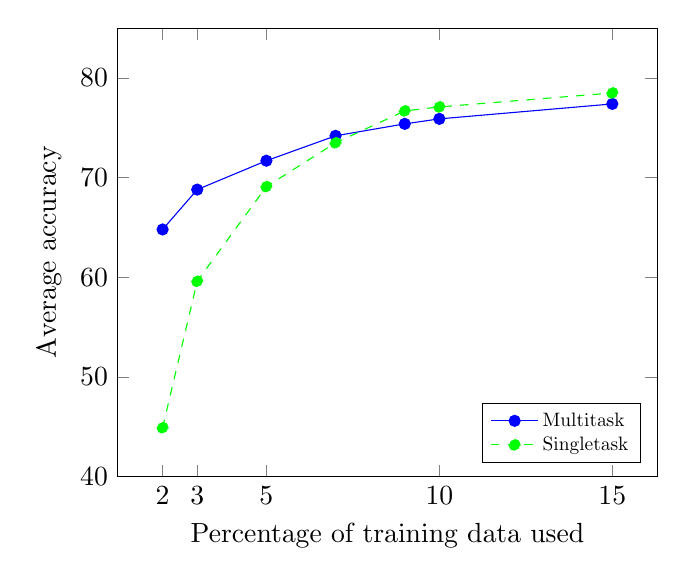
\begin{tikzpicture}
\label{fig:mtl_dialog_part}
\begin{axis}[xlabel = Percentage of training data used,
ylabel = Average accuracy,
legend pos= south east,
% width=10cm,
% height=10cm,
% xmin=2,
% xmax=100,
xtick={2,3,5,10,15},
ymin=40,ymax=85,
legend cell align={left},
legend style={nodes={scale=0.7, transform shape}}
]
\addplot[color=blue,solid, mark=*] coordinates {
(2, 64.8)%50
(3, 68.8)%50
(5, 71.7)%100
(7,74.2)
%(7.5,74.6)
% (8,74.9)
(9,75.4)
(10, 75.9)%300
(15, 77.4)
};
\addlegendentry{Multitask}
\addplot[color=green,dashed,mark=*] coordinates {
(2, 44.9)%50
(3, 59.6)%100
(5, 69.1)%300
(7,73.5)
%(7.5,73.5)
% (8,73.8)%500
(9,76.7)
(10,77.1)
(15, 78.5)
};
\addlegendentry{Singletask}
\end{axis}%
\end{tikzpicture}%
\end{figure}

 
 %TODO - Italicize all backbones? 
\end{table*}
\begin{table*}
\caption{Точность/ F1.  Режим M означает многозадачные модели, режим S означает однозадачные модели, и Доля означает долю использованных тренировочных данных. Базовая модель distilbert. Усреднено по пяти запускам. }
\label{tab:mtl_dialog_part}
\resizebox{\textwidth}{!}{%
\begin{tabular}{c|c|c|c|c|c|c|c|c}
\hline
 \multirow{2}{*}{Режим} &  \multirow{2}{*}{Доля} &  \\multirow{2}{*}{Среднее} & Эмоции & Тональность & Токсичность & Интенты & Темы & Число \\
& & & 39.4k & 80.5k & 127.6k & 11.5k & 11.5k & seen \\
\hline 
S & 15\% & 78.5/70.9 & 65.8/50.6 & 69.3/68.8 & 92.2/81.2 & 78.7/68.8 & 86.3/85.1 & 2173 \\ \hline
M & 15\% & 77.4/70.6 & 64.0/55.0 & 68.3/67.7 & 91.6/80.0 & 76.9/64.6 & 86.4/85.4 & 4741 \\ \hline
S & 10\% & 77.1/68.4 & 64.6/45.0 & 68.3/67.8 & 92.2/81.0 & 75.5/64.7 & 84.8/83.3 & 1579 \\ \hline
M & 10\% & 75.9/69.1 & 62.6/53.6 & 66.6/65.8 & 91.5/79.7 & 74.3/63.2 & 84.6/83.3 & 4295 \\ \hline
S & 9\% & 76.7/67.4 & 64.6/43.9 & 68.2/67.7 & 91.8/80.4 & 74.4/62.7 & 84.2/82.4 & 1457 \\ \hline
M & 9\% & 75.4/67.8 & 62.1/52.4 & 66.5/65.7 & 91.4/79.5 & 72.4/58.5 & 84.4/83.0 & 3695 \\ \hline
%S & 8\% & 73.8/64.6 & 63.7/43.5 & 67.6/67.0 & 92.0/80.5 & 62.0/49.7 & 83.9/82.1 & 1381 \\ \hline
%M & 8\% & 74.9/67.2 & 61.7/51.4 & 66.7/66.0 & 91.5/79.5 & 71.1/57.3 & 83.6/81.7 & 3511 \\ \hline
%S & 7.5\% & 73.5/64.0 & 63.8/42.5 & 67.4/66.9 & 91.6/80.1 & 61.3/48.6 & 83.6/81.7 & 1293 \\ \hline
%M & 7.5\% & 74.6/66.9 & 61.0/50.2 & 67.0/66.4 & 91.5/79.5 & 70.3/56.9 & 83.2/81.4 & 2995 \\ \hline
S & 7\% & 73.5/64.0 & 63.3/42.1 & 67.9/67.4 & 91.8/80.1 & 61.4/49.4 & 83.3/81.1 & 1251 \\ \hline
M & 7\% & 74.2/66.4 & 61.1/50.4 & 65.8/65.1 & 91.0/78.9 & 70.0/56.3 & 83.1/81.3 & 2882 \\ \hline
S & 5\% & 69.1/59.0 & 62.5/38.9 & 66.9/66.3 & 91.8/79.9 & 42.7/30.8 & 81.6/78.8 & 901 \\ \hline
M & 5\% & 71.7/62.4 & 60.5/48.6 & 64.4/63.4 & 90.8/78.5 & 62.4/44.4 & 80.2/77.3 & 2381 \\ \hline
S & 3\% & 59.6/49.0 & 60.6/37.7 & 65.2/64.5 & 91.8/79.3 & 26.5/16.9 & 54.0/46.5 & 584 \\ \hline
M & 3\% & 68.8/58.1 & 58.6/42.7 & 62.5/61.3 & 91.0/78.3 & 55.5/37.1 & 76.4/71.0 & 1566 \\ \hline
S & 2\% & 44.9/31.5 & 48.7/21.7 & 39.6/26.5 & 91.8/79.0 & 2.6/0.2 & 41.4/30.1 & 274 \\ \hline
M & 2\% & 64.8/52.1 & 57.6/38.4 & 61.4/60.1 & 90.8/78.0 & 44.2/23.5 & 69.9/60.4 & 923 \\ \hline
\end{tabular}
}
\end{table*}


Другим интересным направлением исследований является исследование переноса знаний между английским и русским языками в многозадачных моделях. Для исследования данного переноса автор диссертационной работы использовал мультиязыковые базовые модели, предобучавшиеся на большом числе языков. 


\subsection{Многоязычные многозадачные модели - эффект кросс-языкового обучения}

На этой стадии экспериментов, использовались только многоязычные модели. В качестве многоязычных базовых моделей использовались \textit{distilbert-base-multilingual-cased} и \textit{bert-base-multilingual-cased}. На этом этапе решались следующие задачи:

 \begin{itemize}
\item[*] Сравнить качество многозадачных и однозадачных моделей для русского языка при использовании многоязычных базовых моделей. 
\item[*] Проверить, как меняются результаты у однозадачных и у многозадачных моделей, если добавлять при их обучении к русскоязычным данным англоязычные данные, объединяя данные по задаче(то есть для каждой задачи, учить модель на английских и русских данных, но валидировать только на русских). 
\item[*] Проверить, дает ли для описанного в предыдущем пункте какое-то улучшение, если считать англоязычные задачи отдельными задачами (валидируясь все так же только на русскоязычные данных), и соответственно, при обучении на русскоязычных задачах использовать только русскоязычные данные, а при англоязычных - только англоязычные. 
\end{itemize} 

Заметим, что так как англоязычных открытых данных для большинства задач гораздо больше, чем русскоязычных, именно изучение переноса знаний с английского языка на русский представляет бОльший практический интерес, чем изучение переноса знаний с русского языка на английский. Хотя в разделе \ref{ch:yaqtopics} изучается и такой перенос знаний тоже. 
%TODO. Формат представления Accuracy /f1 - должен быть единообразным по диссеру? 
%TODO. Выделять режимы экспериментов в таблицах и перед ними через Italic? 
\begin{table*}
\caption{Точность/f1 macro на русскоязычных данных для многоязычных моделей. Режим S означает однозадачные модели, режим M - многозадачные модели. RU означает русскоязычные данные , EN означает англоязычные данные. Объединенные означает, что русскоязычные и англоязычные данные объединены по задаче, Отдельные означает, что русскоязычные и англоязычными задачи считаются отдельными задачами. Усреднено по трем запускам. }
\label{mult_results}
%\begin{tabular}{|c|c|c||c|c|c|c|c|c|} \hline
\scalebox{0.8}{
\begin{tabular}{|c|c|c||c|c|c|c|c|c||c|} \hline
Модель & \begin{tabular}[c]{@{}l@{}}Тренировочные\\данные\end{tabular} & Режим & Среднее & \begin{tabular}[c]{@{}l@{}}Эмоции\end{tabular} & \begin{tabular}[c]{@{}l@{}}Тональность\end{tabular} & \begin{tabular}[c]{@{}l@{}}Токсичность\end{tabular} & \begin{tabular}[c]{@{}l@{}}Интенты\end{tabular} & \begin{tabular}[c]{@{}l@{}}Темы\end{tabular} &\begin{tabular}[c]{@{}l@{}}Число\\батчей\end{tabular} \\
\hline \hline
\textit{distilbert-base-multilingual-cased} & RU & S & 84.7/81.0 & 77.4/69.1 & 77.7/77.9 & 96.7/94.8 & 83.5/76.6 & 88.1/86.9 & 10058 \\ \hline
\textit{distilbert-base-multilingual-cased} & RU & M & 84.3/80.2 & 78.1/70.5 & 76.8/76.7 & 96.5/94.4 & 81.9/72.3 & 88.2/87.1 & 9821 \\ \hline
\textit{distilbert-base-multilingual-cased} & \begin{tabular}[c]{@{}l@{}}RU+EN,\\объединенные\end{tabular} & S & 85.2/81.8 & 78.9/70.2 & 77.4/77.3 & 96.8/94.9 & 84.7/79.1 & 88.4/87.4 & 31843 \\ \hline
\textit{distilbert-base-multilingual-cased} & \begin{tabular}[c]{@{}l@{}}RU+EN,\\объединенные\end{tabular} & M & 84.5/81.1 & 77.9/70.7 & 76.6/76.7 & 96.5/94.5 & 82.9/76.5 & 88.4/87.2 & 17790 \\ \hline
\textit{distilbert-base-multilingual-cased} & \begin{tabular}[c]{@{}l@{}}RU+EN,\\отдельные\end{tabular} & M & 84.4/80.6 & 77.6/70.0 & 76.8/77.1 & 96.5/94.5 & 82.4/73.9 & 88.3/87.2 & 23688 \\ \hline
\textit{bert-base-multilingual-cased} & RU & S & 84.7/80.2 & 76.6/64.2 & 77.8/78.2 & 96.9/95.1 & 83.9/76.3 & 88.4/87.0 & 10884 \\ \hline
\textit{bert-base-multilingual-cased} & RU & M & 84.8/81.4 & 78.4/71.4 & 76.3/76.3 & 96.8/94.8 & 83.7/76.6 & 89.0/87.8 & 12810 \\ \hline
\textit{bert-base-multilingual-cased} & \begin{tabular}[c]{@{}l@{}}RU+EN,\\объединенные\end{tabular} & S & 85.6/82.3 & 78.9/70.1 & 77.6/77.8 & 96.9/94.9 & 85.0/80.4 & 89.4/88.5 & 23752 \\ \hline
\textit{bert-base-multilingual-cased} & \begin{tabular}[c]{@{}l@{}}RU+EN,\\объединенные\end{tabular} & M & 85.2/82.3 & 79.2/72.7 & 76.4/76.6 & 96.7/94.8 & 84.3/79.3 & 89.4/88.3 & 20755 \\ \hline
\textit{bert-base-multilingual-cased} & \begin{tabular}[c]{@{}l@{}}RU+EN,\\отдельные\end{tabular} & M & 85.0/81.6 & 78.3/71.4 & 77.1/77.0 & 96.7/94.7 & 84.0/76.7 & 89.1/88.0 & 22701 \\ \hline
\end{tabular}
}
\end{table*}

Как можно видеть, результаты для каждого из экспериментов в этой серии доволтно
As we see, the results of all settings are pretty similar: using Russian+English data puts us on the plateau, while improvements are only moderate. Treating English tasks as separate tasks does not bring out improvements, and brings out even a small deterioration. 

In the same setting, we also explored whether utilizing English-language tasks as separate tasks is more beneficial than merging the English data and Russian data by task. This approach did not prove to be any better or worse.

The exact exploration of the impact of adding English data where we have limited Russian data (like in most cases) requires additional investigation, which was done in the next series of experiments. The real-world situation is that we usually have a huge body of datasets for English data, but not nearly as much for Russian data. This gives additional practical value to that experiments. 

\subsection{When the adding of English data helps?}

In this experiment series, we explore multi-task settings with merged labels. We study how much improves the performance of multilingual distilbert (multi-task or singletask), trained on some share of Russian train data if we add English training data to this share of Russian train data and validate on the English validation data. 

Specifically, we performed experiments for the following data shares: 0\%,3\%, 5\%, 15 \%, 20\%, 25\%, 50\%, and 100\%. For 0\%, we added to the table the model trained on English train data and validated on Russian validation data, and the model which is trained on English train data and validated on English validation data (but tested still on Russian test data). We restarted the experiments with three random seeds. For every series of experiments, we randomly shuffled the datasets and then selected all subsets at once, while the larger subsets contained all examples from the smaller subsets (like, 10\% subset contains all examples from 5\% and also from 3\%)

We present the averaged results in ~\ref{mult_smalldata_results}, in Appendix. We averaged the results by three runs. For training on the 3-5\% of the Russian data without the English data, we averaged the results by five runs due to the high variability of results. We plot the results below, in~\ref{fig:thresholds_acc}. The task-wise results for the Russian data are also plotted in Appendix.

We also note that in the settings where 100\% share of the English data was used, we performed the experiments also with validation on the Russian data instead of the English data. That change did not impact the scores in any meaningful way.

\begin{figure}[ht]
    \includegraphics[width=\textwidth]{thresholds_acc_ru.jpg}
  \caption{Singletask and multi-task accuracy, while using some share of Russian training data alone or augmenting them with the full English data in "merged by task" mode.}\label{fig:thresholds_acc}
\end{figure}
\begin{figure}[ht]
    \includegraphics[width=\textwidth]{acc_ru_by_task_n_samples.jpg}
  \caption{Singletask and multi-task accuracy, while using some share of Russian training data alone, depending on the number of samples. Accuracies are provided for every task, average accuracy is also provided for comparison to be more convenient.}\label{fig:accuracy_by_task_n_samples}
\end{figure}

%\begin{figure}[ht]
%    \includegraphics[width=\textwidth]{plot}
%  \caption{Singletask and multi-task f1 macro, while using some share of Russian training data alone or augmenting them with the full English data in "merged by task" mode.}\label{fig:thresholds_f1_macro}
%\end{figure}

 

\section{Выводы и анализ результатов}
% объединить 2 секции в 1

Based on the metrics on the diverse set of dialog-related tasks, the proposed multi-task transformer-agnostic model almost matches the single-label model. 
For all explored BERT-based backbones the drop in average accuracy is between 0.8\%-0.9\% on the dialogue tasks.

For the GLUE tasks, the multi-task models even exceed the single-task ones by average accuracy. This applies to GLUE tasks with not large enough training sets (AX, STS-B, and especially RTE) which benefit from knowledge transfer from large-scale tasks (MNLI, QQP).
%Distilbert-like models almost match the bert-like ones by their overall performance, for single-task and multi-task settings.
The training of the multi-task neural network, however, took more training steps than the training of the corresponding single-task models with the same early stopping criteria. The reason is that the training did not stop until the metrics on relatively small-data tasks stopped improving. 
% Therefore, examples from relatively high-size tasks, metrics for which had already reached their saturation points, were seen more frequently than they would have been seen if the model was single-task and trained for any of these tasks. If we train on the data subsets, this effect is more pronounced, probably because the gap between the saturation points from smaller-data tasks and larger-data tasks widens.
From all the tasks, the dropdown is the lowest on the topic classification tasks, which suggests that this task is more prone to knowledge transfer.

For the small-scale data, we can see that if we train on small shares of training data (2-5\%), multi-task models overcome single-task models, for 2\% and 3\% -- by a huge margin. However, even on 9\%, for all dialog tasks, this advantage eliminates.

The multi-task small-scale advantage in accuracy strongly depends on the data size. For the toxicity classification (127k samples), single-task models excel multi-task ones even at 2\% data. For the sentiment and emotion classification (79.2k and 39.3k), the advantage starts at 3\%, for topic classification (11.5k) at 5\%, and for intent classification (11.5k) at 9\%. 

Therefore, the smaller the auxiliary dataset (on the scale of ~200-2000 samples), the larger the advantage of multi-task models. This advantage shows that the knowledge transfer effect is the most noticeable for small-scale datasets.

Also, the difference between metrics of the topic classification and intent classification makes us suppose that the advantage of multi-task training depends not just on the number of samples, but on the number of samples per class. Testing this hypothesis, however, might require additional investigation. 

We also leave exploring whether these conclusions hold for the different task types, for example, sequence tagging and question answering, as a subject of future research. Testing these 
conclusions on other languages or on other transformer-based models (for example, decoder-base ones)  is also a possible future field of study.

.
Multi-task transformer-agnostic models almost match the singletask models by metrics on the dialog tasks. The accuracy gap between the multi-task and singletask monolingual models is about 0.8-0.9\% for the English language and about 0.3-0.6\% for the Russian language. For the multilingual models, the gap remains within the same limit, except for the multilingual BERT trained on Russian data, where the gap evaporates completely.

% We also report that the training of the multi-task neural network for English data took 21-24\% more training steps than the training of the singletask models with the same criteria of early stopping. The reason is that the model did not stop until the metrics on relatively low-size tasks stop improving, therefore examples from relatively high-size tasks that already were trained) were seen more times than they would have been seen if the model was singletask and trained for any of these tasks. Убрать вообще batches seen, раз не видно паттерна?

We also show that if we have Russian and English data for the same tasks, it does not matter match whether we unite data for every task, or we treat them as separate tasks. The choice of sampling, between plain, uniform, and annealed, also did not matter match in our experiments; however, this might also indicate that annealed sampling requires thorough tuning of hyperparameters.

For the small-scale data, we can see that if we train the multilingual distilbert on small shares of Russian training data (2-5\%), multi-task models overcome singletask models in the average accuracy. As shown in Figure 2, this accuracy advantage strongly depends on the dataset size - the smaller the truncated dataset size, the larger the advantage. For intent and topic datasets this advantage evaporates at 1151 training samples, but for the emotion dataset, surprisingly, this advantage holds true with any dataset partition, possibly due to the effect of knowledge transfer from the sentiment task.

The hypothesis of the knowledge transfer dependency of the dataset size is additionally supported by the fact that for experiments with adding English data, multi-task models showed no clear pattern of advantage over singletask ones.

We also find that while having a limited amount of Russian training data (3-10\% RU share in Table 4 from Appendix)  we can additionally improve the multi-task BERT metrics up to several percent if we add the English data to the training sample. 

And in this case, we can also perform the validation on the English validation data, it does not change metrics in a meaningful way compared to the validation on the Russian validation data set. 

And also, the lower share of training data we have, the larger the accuracy gain for adding the English data to the training sample.


\section{Conclusion}

The proposed transformer-agnostic multi-task models yield results matching or approaching the single-task models on most tasks. If we truncate the tasks to the low-size number (200-2000 samples), multi-task models start exceeding the single-task ones. This effect might depend on the number of samples per class.
\fi
The multi-task transformer-agnostic architecture we propose yields just a minor decrease in accuracy and F1 macro on the dialog tasks compared to the singletask architecture. 

Adding English data to the Russian dataset can improve the metrics by up to several percent for the singletask and multi-task training. Also, starting from some data sizes, multi-task architecture starts overcoming the singletask one.


\chapter{Исследование переноса знаний в многоязычных моделях на новом тематическом наборе данных}\label{ch:rutopics}
\section{Введение}
В предыдущей главе \ref{ch:tr-ag} был исследован перенос знаний в многозадачных многоязычных моделях. Тем не менее, в этой главе остался не исследован перенос знаний с русского языка на другие языки. Также, в этой главе осталось не раскрыто то, от чего зависит качество переноса знаний в многоязычных моделях на разные языки.
Помимо этого, прикладные задачи диалоговой платформы {DREAM} требовали создания русскоязычного набора данных для тематической классификации, которые подходят к применению в реальных диалоговых системах. Существующие наборы данных для тематической классификации, поддерживающие русский язык, имеют следующие проблемы:
\begin{itemize}
   \item[*] Часть таких наборов данных состоит из длинных обучающих примеров(как правило - новостей). Опыт применения моделей, обученных на наборе данных {DeepPavlov Topics} в диалоговой платформе DREAM, показывает(см. главу \ref{ch:mtldream}), что модели, обученные на таких данных, могут переобучаться на них и плохо себя показывать на реальных диалоговых задачах. Примерами таких наборов данных являются {MLSUM}~\cite{mlsum} и {XGLUE-nc}~\cite{xglue}.
   \item[*] Часть таких наборов данных является слишком специфичными и хорошо подходят для классификации узкоспециализированных вопросов, но не подходят для классификации широкого спектра тем из-за специфичной номенклатуры классов.  Примерами таких наборов данных являются~\cite{healthcare_facilities_reviews} и  ~\cite{pstu}
   \item[*] Некоторые наборы данных для тематической классификации лишены этих проблем, но либо имеют слишком маленькое число примеров~\cite{chatbotru}, либо имеют номенклатуру классов, далекую от покрытия всех потребностей диалоговой системы~\cite{massive}.
\end{itemize}
Данные вопросы были подробно освещены в статье \cite{rutopics}, по материалам которой написана данная глава. 

\textbf{Задачи}, поставленные в данной главе:
\begin{enumerate}
  \item \textbf{Проверить пригодность русскоязычного открытого набора тематических данных для решения задачи русскоязычной тематической классификации и фундаментальных задач исследования переноса знаний на разговорных данных.}
  \item \textbf{Проверить зависимость межъязыкового переноса знаний на разговорных данных в многоязычных нейросетевых моделях от размера предобучающей выборки и генеалогической близости языков к языку дообучения.}
  \end{enumerate}

В качестве языка дообучения в данной главе использовался только русский язык. Использование других языков в качестве языков дообучения требует дополнительных исследований.

\section{Набор данных {YAQTopics}}

В работе изучается русскоязычный набор данных для тематической классификацииt - {YAQTopics}.
\subsection{Получение набора данных}
Этот набор данных с сервиса «Яндекс. Кью»~\cite{yandex_q} был получен по данной ссылке:\url{https://huggingface.co/datasets/its5Q/yandex-q/blob/main/full.jsonl.gz}.

В данный набор данных были включены примеры из 76 разных тем. Выбор тем осуществлялся, основываясь на наборе данных {DeepPavlov Topics} и потребностях диалоговой платформы \textbf{DREAM}. Тема каждого вопроса соответствовала теме этого вопроса из «Яндекс. Кью». Некоторые из выбранных тем могут быть похожими друг на друга, как и реальные темы из «Яндекс. Кью» - следовательно, прикладное использование набора данных {YAQTopics} может требовать объединения некоторых тем.

 Для каждого вопроса, выбирался также ответ наилучшего качества (или первый из таких ответов, если их было несколько). Для части вопросов ответ был пустым. 
 

% TODO ВЫБОРКА ТЕСТОВАЯ ВАЛИДАЦИОННАЯ ИЛИ РАЗБИЕНИЕ? singlelabel multilabel перевод) однометочная? многометочная? Формат чисел. {DREAM} - жирным

% TODO. CHECK THE TOPIC NUMBER. PROVIDE a LINK TO EVERY QUESTION in the final dataset version. 
\subsection{Разбиение и размеры}
Полученные пары вопрос-ответ были разбиты на две части. В часть 1 (однометочную) попали только те пары, в которых вопрос принадлежит только к одной теме, и при этом ответ на этот вопрос либо не существует, либо может быть найден только в этой же теме. Все остальные примеры принадлежат части 2 (многометочной). Все эксперименты, описанные в данной главе, проводились только с примерами из однометочной части {YAQTopics}.


Для всех тем, было выбрано 532590 уникальных вопросов, из которых 403938 было отвечено. При этом однометочная часть набора данных содержит 361650 вопросов, из которых 266597 было отвечено. Многометочная часть, в свою очередь, содержит 170930 вопросов, из которых 137431 было отвечено.
%todo - YAQTOPICS одними и теми же буквами как в статтк

Помимо этого, из однометочной части {YAQTopics} была дополнительно выделена равноразмерная часть данного набора данных. Если вопрос отвечен и суммаризованная версия вопроса при этом встречается только в одной теме (той же, что и тема ответа), то данный вопрос вместе с ответом и суммаризованным ответом включается не только в однометочную часть {YAQTopics}, но и в равноразмерную часть этого набора данных.
 
Размеры всех частей {YAQTopics} как для всего набора данных, так и для каждого из классов, с которыми проводились описанные в данной главе эксперименты, включены в Таблицу~\ref{tab:rutopics:sizes}.

%TODO
\begin{table}[t]
\centering
\scalebox{0.7}{
\begin{tabular}{|c||c|c|c|c|c|}
\textbf{тип данных}  & \multicolumn{2}{c|}{\textbf{однометочные}} & \multicolumn{2}{c|}{\textbf{многометочные}} & \multirow{2}{*}{\textbf{равноразмерные}}\\
\cline{1-5}
\textbf{класс}  & \multicolumn{1}{c|}{все} & \multicolumn{1}{c|}{отвеченные} & \multicolumn{1}{c|}{все} & \multicolumn{1}{c|}{отвеченные} & \\\hline \hline
\textit{Размер набора данных} & 361650 & 266597 & 170930 & 137341 & 264786\\ \hline
\textit{Размер 6классового поднабора данных} & 18864 & 15912 & 27191 & 20569 & 15830 \\ \hline
\textit{Музыка} & 9514 & 5809 & 4456 & 3287 & 5797 \\ \hline
\textit{Еда, напитки и кулинария} & 5750 & 4758 & 14096 & 11084 & 4723 \\ \hline
\textit{Медиа и коммуникации} & 4505 & 2637 & 5577 & 3948 & 2619 \\ \hline
\textit{Транспорт} & 2435 & 1625 & 1933 & 1387 & 1613 \\ \hline
\textit{Новости} & 945 & 602 & 912 & 720 & 600\\ \hline
\textit{Погода} & 890 & 481 & 217 & 143 & 478 \\ \hline
    
\end{tabular}
}
\caption{Размеры набора данных {YAQTopics} по классу и части}
%\centering
\label{tab:rutopics:sizes}
\end{table}


\section{Выбор представления набора данных {YAQTopics}}\label{rutopics:prepr}

После получения набора данных {YAQTopics}, было необходимо выбрать метод предобработки данного набора данных, показывающий наилучшие результаты на разговорных задачах. Проводилось сравнение следующих трех методов предобработки:

\begin{itemize}
   \item \textbf{Q} означает использование только вопросов.
   \item \textbf{A} означает использование только ответов.
   \item \textbf{Q [SEP] A} означает, что если ответ на вопрос существует, используется конкатенация вопроса с ответом на этот вопрос при помощи токена [SEP]. Иначе используется просто вопрос.  
\end{itemize}

В предварительных экспериментах, вместо ответов использовались их суммаризованные версии. Суммаризация проводилась при помощи алгоритма TextRank~\cite{summarizer}. Использование только суммаризованных ответов показало стабильно худшие результаты, чем использование только несуммаризованных. При этом конкатенация вопросов к суммаризованным ответам не дает устойчивых изменений качества по сравнению с конкатенацией вопросов к ответам.

Для всех методов предобработки, обучение проводилось на равноразмерной версии {YAQTopics}(колонка «равноразмерные» из Таблицы~\ref{tab:rutopics:sizes}).
Такой режим обучения позволяет проводить честное сравнение между признаками, полученными разными методами предобработки, так как количество тренировочных примеров при данном режиме то же самое безотносительно способа предобработки данных. Результаты сравнения вышеупомянутых методов предобработки приводятся в Таблице~\ref{tab:rutopics:matched}. В этой таблице и всех таблицах этого раздела макро-усредненное f1 обозначается как f1.
 \subsection{Как сравнить представления набора данных друг с другом?}
Для оценки любого из упомянутых выше методов предобработки набора данных, модель для сравнения обучалась на тренировочных примерах из {YAQTopics}, принадлежащих любому из соответствующих набору данных {MASSIVE} шести классов и полученных в соответствии с этим методом. Валидация производилась на примерах из валидационной части MASSIVE, принадлежащих вышеупомянутым шести классам. После завершения обучения, данная модель оценивалась на поднаборе тренировочных+тестовых примеров из русского {MASSIVE}, принадлежащих соответствующим шести классам из этого набора данных. Этот поднабор обозначается как «объединенные тестовые данные».

При сравнении набора данных {YAQTopics} с набором данных {MASSIVE}, можно видеть, что только шесть классов из {MASSIVE} можно поставить в соответствие классам из  {YAQTopics}. Следовательно, нейросетевая модель в данных экспериментах обучалась только для шести соответствующих классов {YAQTopics}: \textit{Еда, напитки и кулинария} (соответствует классу \textit{cooking} из {MASSIVE}), \textit{Новости} (соответствует классу \textit{news} из {MASSIVE} ), \textit{Транспорт} (соответствует классу \textit{transport} из {MASSIVE}), \textit{Музыка} (соответствует классу \textit{music} из {MASSIVE}),\textit{Медиа и коммуникации} (соответствует классу \textit{social} из {MASSIVE}) и \textit{Погода} (соответствует классу \textit{weather} из {MASSIVE} class). Классы из набора данных {YAQTopics} никак не объединялись, хотя это предположительно могло бы дополнительно улучшить результаты на классах \textit{cooking} и \textit{transport} из набора данных {MASSIVE}.

Этот метод позволяет проверить пригодность набора данных {YAQTopics} для разговорной тематической классификации - по крайней мере, на выбранных шести классах. Впрочем, так как примеры для всех шести классов были получены похожим образом, можно ожидать, что другие классы из {YAQTopics} настолько же хорошо подходят для разговорной тематической классификации.

\subsection{Описание экспериментов для сравнения}
Эксперименты, описанные в Таблице~\ref{tab:rutopics:matched}, проводились на различных базовых моделях из библиотеки {Transformers}~\cite{huggingface_transformers} от HuggingFace : \textit{bert-base-multilingual-cased}~\cite{multilingual_bert}, \textit{DeepPavlov/distilrubert-tiny-cased-conversational}~\cite{distilrubert}, \textit{sberbank-ai/ruBert-base}~\cite{sbert_base}  \textit{DeepPavlov/rubert-base-conversational-cased}~\cite{rubert}. Все эти модели имеют архитектуру типа BERT. Последние 2 модели очень похожи, но имеют несколько отличающееся число параметров, так как в них применяются разные методы токенизации.

Данные всех экспериментов, описанных в этой главе, приведены в Таблице~\ref{appendix:rutopics:allruns}. 

Подробное сравнение всех базовых моделей приведено в Таблице~\ref{tab:rutopics:backbones}.

\begin{table*}
\centering
\resizebox{\textwidth}{!}{
\begin{tabular}{|c|c|c|c|c|}
\hline
\multirow{1}{*}{\textbf{Модель}} & \multirow{1}{*}{\textbf{Сокращение}}  & \textbf{Многоязычность} &  \multicolumn{1}{c|}{\textbf{Число слоев}} & \textbf{Parameters}\\ \hline
\textit{DeepPavlov/distilrubert-tiny-cased-conversational}~\cite{distilrubert} & \textit{rubert-tiny} & нет & 2 & 107M\\ \hline
\textit{DeepPavlov/rubert-base-cased-conversational}~\cite{rubert} & \textit{rubert} & нет & 12 & 177.9M\\ \hline
\textit{bert-base-multilingual-cased}~\cite{multilingual_bert} & \textit{multbert} & да & 12 & 177.9M \\ \hline
\textit{sberbank-ai/ruBert-base}~\cite{sbert_base} & \textit{ru-sbert} & да & 12 & 178.3M\\ \hline
\end{tabular}
}
\caption{Параметры различных базовых моделей, рассмотренных в этой главе}
\label{tab:rutopics:backbones}
\end{table*}

\begin{table*}
\centering
\caption{ Точность (макро-F1) различных типов базовых моделей на объединенных тестовых данных {MASSIVE} для русского языка.
Модели были обучены на шестиклассовой \textbf{равноразмерной} подвыборке {YAQTopics}, предобработанной при помощи одного из нескольких режимов, описанных в Разделе~\ref{rutopics:prepr}. Условные обозначения моделей - как в  Таблице~\ref{tab:rutopics:backbones}. Усреднено по трем запускам.}
\scalebox{0.65}{
\label{tab:rutopics:matched}
\begin{tabular}{|c|c||c|c|c|c|c|c|c|c|c|c|c|c|c|c|}
\hline
\multirow{2}{*}{\textbf{Модель}} & \multirow{2}{*}{\textbf{Режим}}  &  \multicolumn{2}{c|}{\textbf{Все классы}} &  \multicolumn{2}{c|}{\textbf{music}} &  \multicolumn{2}{c|}{\textbf{cooking}} &  \multicolumn{2}{c|}{\textbf{news}} &  \multicolumn{2}{c|}{\textbf{transport}} &  \multicolumn{2}{c|}{\textbf{weather}} &  \multicolumn{2}{c|}{\textbf{social}} \\ 
\cline{3-16}
& & Точность & Macro-F1 & Точность & F1 & Точность & F1 & Точность & F1 & Точность & F1 & Точность & F1 & Точность & F1 \\ \hline
\textit{ru} &  \textbf{Q} & 85.0 & 84.3 & 94.7 & 87.5 & 98.4 & 86.0 & 82.5 & 82.7 & 92.1 & 92.1 & 82.5 & 89.6 & 66.1 & 68.0\\ %\hline
\textit{rutiny} &  \textbf{Q} & 85.7 & 85.2 & 95.0 & 87.5 & 98.7 & 87.3 & 82.2 & 82.9 & 92.8 & 92.3 & 84.3 & 90.6 & 67.3 & 70.3\\ %\hline
\textit{rusber} &  \textbf{Q} & 85.5 & 84.9 & 93.7 & 89.9 & 98.8 & 87.2 & 83.0 & 83.1 & 93.1 & 91.1 & 85.1 & 91.1 & 64.3 & 67.2\\ %\hline
\textit{mult} &  \textbf{Q} & 80.8 & 79.8 & 94.3 & 77.3 & 97.2 & 82.8 & 75.5 & 81.1 & 90.0 & 90.5 & 78.5 & 86.0 & 57.5 & 61.0\\ \hline
\textit{ru} &  \textbf{A} & 79.8 & 77.9 & 95.8 & 79.0 & 98.9 & 75.2 & 65.9 & 76.7 & 90.2 & 88.3 & 85.0 & 90.3 & 51.0 & 57.8\\ %\hline
\textit{rutiny} &  \textbf{A} & 82.4 & 80.9 & 96.1 & 81.8 & 99.3 & 78.2 & 72.8 & 81.2 & 88.6 & 89.8 & 87.2 & 91.2 & 57.9 & 63.3\\ %\hline
\textit{rusber} &  \textbf{A} & 82.6 & 80.9 & 94.3 & 83.4 & 98.9 & 80.8 & 74.4 & 80.2 & 90.6 & 89.4 & 89.3 & 90.9 & 52.7 & 60.6\\ %\hline
\textit{mult} &  \textbf{A} & 74.5 & 72.9 & 95.8 & 69.6 & 95.9 & 72.1 & 66.1 & 75.5 & 80.4 & 83.3 & 76.7 & 83.4 & 44.0 & 53.6\\ \hline
\textit{ru} &  \textbf{Q [SEP] A} & 85.4 & 84.9 & 94.0 & 88.5 & 97.6 & 87.1 & 82.5 & 83.7 & 93.1 & 91.5 & 83.6 & 90.0 & 67.1 & 68.8\\ %\hline
\textit{rutiny} &  \textbf{Q [SEP] A} & 85.3 & 84.7 & 94.3 & 87.4 & 97.9 & 86.4 & 79.3 & 81.4 & 91.6 & 92.8 & 86.0 & 91.0 & 68.2 & 69.1\\ %\hline
\textit{rusber} &  \textbf{Q [SEP] A} & 85.1 & 84.2 & 93.1 & 91.6 & 98.3 & 88.4 & 88.1 & 81.2 & 93.3 & 91.9 & 86.2 & 91.6 & 53.7 & 60.7\\ %\hline
\textit{mult} &  \textbf{Q [SEP] A} & 80.0 & 79.7 & 94.2 & 77.0 & 95.1 & 85.5 & 74.9 & 80.3 & 87.8 & 88.0 & 73.8 & 83.8 & 64.6 & 63.6\\ \hline
\end{tabular}
}
\end{table*}

\begin{table*}
\centering
\caption{ Точность (макро-F1) различных типов базовых моделей на объединенных тестовых данных {MASSIVE} для русского языка.
Модели были обучены на шестиклассовой \textbf{полной} подвыборке {YAQTopics}(из всей однометочной части), предобработанной при помощи одного из нескольких режимов, описанных в Разделе~\ref{rutopics:prepr}. Условные обозначения моделей - как в  Таблице~\ref{tab:rutopics:backbones}. Усреднено по трем запускам.}
\scalebox{0.65}{
\label{tab:rutopics:full}
\begin{tabular}{|c|c||c|c|c|c|c|c|c|c|c|c|c|c|c|c|}
\hline
\multirow{2}{*}{\textbf{Модель}} & \multirow{2}{*}{\textbf{Режим}}  &  \multicolumn{2}{c|}{\textbf{Все классы}} &  \multicolumn{2}{c|}{\textbf{music}} &  \multicolumn{2}{c|}{\textbf{cooking}} &  \multicolumn{2}{c|}{\textbf{news}} &  \multicolumn{2}{c|}{\textbf{transport}} &  \multicolumn{2}{c|}{\textbf{weather}} &  \multicolumn{2}{c|}{\textbf{social}} \\ 
\cline{3-16}
& & Точность & Macro-F1 & Точность & F1 & Точность & F1 & Точность & F1 & Точность & F1 & Точность & F1 & Точность & F1 \\ \hline
\textit{ru} &  \textbf{Q} & 85.0 & 84.3 & 94.7 & 87.5 & 98.4 & 86.0 & 82.5 & 82.7 & 92.1 & 92.1 & 82.5 & 89.6 & 66.1 & 68.0\\ %\hline
\textit{rutiny} &  \textbf{Q} & 85.7 & 85.2 & 95.0 & 87.5 & 98.7 & 87.3 & 82.2 & 82.9 & 92.8 & 92.3 & 84.3 & 90.6 & 67.3 & 70.3\\ %\hline
\textit{rusber} &  \textbf{Q} & 85.5 & 84.9 & 93.7 & 89.9 & 98.8 & 87.2 & 83.0 & 83.1 & 93.1 & 91.1 & 85.1 & 91.1 & 64.3 & 67.2\\ %\hline
\textit{mult} &  \textbf{Q} & 80.8 & 79.8 & 94.3 & 77.3 & 97.2 & 82.8 & 75.5 & 81.1 & 90.0 & 90.5 & 78.5 & 86.0 & 57.5 & 61.0\\ \hline
\textit{ru} &  \textbf{A} & 79.8 & 77.9 & 95.8 & 79.0 & 98.9 & 75.2 & 65.9 & 76.7 & 90.2 & 88.3 & 85.0 & 90.3 & 51.0 & 57.8\\ %\hline
\textit{rutiny} &  \textbf{A} & 82.4 & 80.9 & 96.1 & 81.8 & 99.3 & 78.2 & 72.8 & 81.2 & 88.6 & 89.8 & 87.2 & 91.2 & 57.9 & 63.3\\ %\hline
\textit{rusber} &  \textbf{A} & 82.6 & 80.9 & 94.3 & 83.4 & 98.9 & 80.8 & 74.4 & 80.2 & 90.6 & 89.4 & 89.3 & 90.9 & 52.7 & 60.6\\ %\hline
\textit{mult} &  \textbf{A} & 74.5 & 72.9 & 95.8 & 69.6 & 95.9 & 72.1 & 66.1 & 75.5 & 80.4 & 83.3 & 76.7 & 83.4 & 44.0 & 53.6\\ \hline
\textit{ru} &  \textbf{Q [SEP] A} & 85.4 & 84.9 & 94.0 & 88.5 & 97.6 & 87.1 & 82.5 & 83.7 & 93.1 & 91.5 & 83.6 & 90.0 & 67.1 & 68.8\\ %\hline
\textit{rutiny} &  \textbf{Q [SEP] A} & 85.3 & 84.7 & 94.3 & 87.4 & 97.9 & 86.4 & 79.3 & 81.4 & 91.6 & 92.8 & 86.0 & 91.0 & 68.2 & 69.1\\ %\hline
\textit{rusber} &  \textbf{Q [SEP] A} & 85.1 & 84.2 & 93.1 & 91.6 & 98.3 & 88.4 & 88.1 & 81.2 & 93.3 & 91.9 & 86.2 & 91.6 & 53.7 & 60.7\\ %\hline
\textit{mult} &  \textbf{Q [SEP] A} & 80.0 & 79.7 & 94.2 & 77.0 & 95.1 & 85.5 & 74.9 & 80.3 & 87.8 & 88.0 & 73.8 & 83.8 & 64.6 & 63.6\\ \hline+-
\end{tabular}
}
\end{table*}

Как можно видеть из Таблицы~\ref{tab:rutopics:matched}, модели, учиышиеся только на ответах, показывают лучшие результаты, чем учившиеся только на вопросах, а учившиеся только на ответах. Это верно для всех рассмотренных базовых моделях, что доказывает: вопросы - самый информативный элемент набора данных {YAQTopics}. 

Конкатенация вопросов к ответам не дает стойкого улучшения по сравнению с использованием только лишь вопросов. 

В общем и целом, все русскоязычные модели показывают похожие результаты, а многоязычная модель ожидаемо показывает результаты хуже, чем любая из русскоязычных. 

Все эти выводы также справедливы для экспериментов, в которых использовались все данные из части 1 набора данных {YAQTopics}, принадлежащие вышеупомянутым шести классам. Данные этих эксперим.

Для дальнейших экспериментов в этой главе был выбран режим предобработки \textbf{Q}, так как остальные режимы либо сложнее и при этом дают результаты не лучше, чем у \textbf{Q} (\textbf{Q [SEP] A}), либо показывают результаты хуже, чем у \textbf{Q} (\textbf{A}).

\section{Оценка для всех классов {YAQTopics}}

Другая важная задача - определение того, как хорошо в принципе могут классы из {YAQTopics} быть различими. Для этого мы проводим кросс-валидацию по 5 разбиениям на тренировочную и валидационнную выборку на данных из всех 76 классов из однометочной части {YAQTopics}.\footnote{Для каждого из разбиений - 80\% данных было тренировочными, 20\% валидационными и они же тестовыми, для разных разбиений это были разные 20\%.} Результаты представлены в Таблице~\ref{tab:crossvalidation}.


\begin{table*}
\centering
\caption{Точность (Макро-F1) различных базовых моделей для 5-кратной кросс-валидации на всех классах из наборе данных {YAQTopics} при обучении только на вопросах.
 Базовые модели обозначаются как в Таблице~\ref{tab:rutopics:backbones}, Разб. означает разбиение. Дисперсия не превосходит 0.65 для всех базовых моделей.}
\scalebox{0.65}{
\label{tab:crossvalidation}
\begin{tabular}{|c||c|c|c|c|c|c|c|c|c|c|c|c|}
\hline
\multirow{2}{*}{\textbf{Модель}} & \multicolumn{2}{c|}{\textbf{Среднее}} & \multicolumn{2}{c|}{\textbf{Разб. 1}} & \multicolumn{2}{c|}{\textbf{Разб. 2}} &\multicolumn{2}{c|}{\textbf{Разб. 3}} & \multicolumn{2}{c|}{\textbf{Разб. 4}} & \multicolumn{2}{c|}{\textbf{Разб. 5}} \\ 
\cline{2-13}
& Точность & Макро-F1 & Точность & Макро-F1 & Точность & Макро-F1 & Точность & Макро-F1   & Точность & Макро-F1 & Точность & Макро-F1 \\ \hline
%\textit{rusber} & 74.0 & 53.4 \\ \hline
%\textit{ru} & 73.7 & 52.5 \\ \hline
%\textit{rutiny} & 72.2 & 50.9 \\ \hline
%\textit{mult} & 71.4 & 51.9 \\ \hline
\textit{rusber} & 74.0 & 53.4 & 73.7 & 54.3 & 73.8 & 52.8 & 73.9 & 53.0 & 74.1 & 54.2 & 74.2 & 52.9\\
\textit{ru} & 73.7 & 52.5 & 73.5 & 52.9 & 73.7 & 51.9 & 73.6 & 52.3 & 73.9 & 53.1 & 73.9 & 52.3\\
\textit{rutiny} & 72.2 & 50.9 & 72.0 & 49.7 & 72.2 & 50.9 & 72.0 & 51.4 & 72.4 & 51.1 & 72.3 & 51.6\\
\textit{mult} & 71.4 & 51.9 & 71.2 & 52.4 & 71.5 & 51.9 & 71.5 & 51.4 & 71.2 & 51.6 & 71.7 & 52.1\\ \hline
\end{tabular}
}
\end{table*}

Результаты могут быть дополнительно улучшены при помощи объединения некоторых классов из похожих тем «Яндекс. Кью». Но даже без этого, русскоязычные недистиллированные базовые модели  показывают точность 73.7-74.0\%, в то время как дистиллированные базовые модели показывают себя несколько хуже (точность 72.2\%). Многоязычная базовая модель ожидаемо показывает себя по этой метрике несколько хуже этих моделей (точность 71.4\%). Это показывает, что тематические классы в этом наборе данных можно отличить друг от друга с достаточно высокой точностью.

\section{Перенос знаний между языками}
После выбора наилучшего метода использования набора данных {YAQTopics}, необходимо было ответить на следующие вопросы:
\begin{itemize}
\item[*]Как эффективно знания из {YAQTopics} переносятся между несколькими языками?
\item[*]Что влияет на эффективность этого переноса?
\end{itemize}
Чтобы ответить на эти вопросы, были получены предсказания модели \textit{bert-base-multilingual-cased} не только для руссского языка, но и для всех языков из набора данных {MASSIVE}. Данная модель обучалась в режиме \textbf{Q} из Таблицы \ref{tab:rutopics:matched}, на всех данных из шести выбранных в предыдущем разделе классов {YAQTopics}, имеющих только одну метку.

Для экспериментов использовалась версия 1.1 {MASSIVE}, содержащая каталанский язык. Так как {MASSIVE} и содержит как современную, так и традиционную версию китайской письменности, учитывались обе. Как и в Таблицах \ref{tab:rutopics:matched} и \ref{tab:rutopics:full}, полученные результаты были усреднены по трем запускам.
%To article - точно work claims?
Полученные результаты представлены в Таблице \ref{tab:rutopics:crosslingual}. Исходя из данной таблицы, можно сделать вывод о корреляции качества многоязычной модели BERT для разных языков с размером обучающей выборки для этих языков. Авторы модели \textit{bert-base-multilingual-cased} утверждают,\footnote{\url{https://github.com/google-research/bert/blob/master/multilingual.md}} что тренировочной выборкой модели \textit{bert-base-multilingual-cased} для каждого языка являлся размер Википедии для этого языка, при этом для обучающей выборки было применено экспоненциальное сглаживание со степенью 0.7 для балансировки языков.
%TO ARTICLE - pretraining sample size. %Smoothing of training sample - expressions as in the url.
Соответственно, в качестве приближения размера Википедии для каждого языка, был выбрано число статей Википедии для этого языка на 11 октября 2018 года(дату выпуска модели BERT), возведенное в степень 0.7.  Число статей Википедии для каждого языка на эту дату также представлено в Таблице~\ref{tab:rutopics:crosslingual}. Помимо этого, в Таблице~\ref{tab:rutopics:crosslingual} также представлена генеалогическая близость каждого языка к русскому, вычисленная в соответствии с работой~\cite{lang_sim}. 

% TODO UPDATE ALL RUNS
\begin{table*}
\caption{Точность (f1) модели \textit{bert-base-multilingual-cased} на объединенном тестовом наборе данных {MASSIVE} для всех языков. Модель обучалась на версии \textbf{Q} набора данных {YAQTopics}.\textbf{Код} означает код языка(ISO 639-1), \textbf{N} означает число статей в Википедии на этом языке на 11 октября 2018 года, \textbf{Дистанция} означает лингвистическую дистанцию между этим языком и русским, посчитанную в соответствии с работой~\cite{lang_sim}. Усреднено по трем запускам.}
\label{tab:rutopics:crosslingual}
\centering
   \scalebox{0.5}{
\begin{tabular}{|c|c|c||c|c|c|} \hline
\multirow{2}{*}{\textbf{Язык}}  & \multirow{2}{*}{\textbf{Код}} & \multirow{2}{*}{\textbf{Дистанция}} & \multirow{2}{*}{\textbf{Число статей}}  &  \multicolumn{2}{c|}{\textbf{Метрики}} \\ %\hline
\cline{5-6}
& & & & Точность & Макро-F1 \\ \hline \hline
русский & ru & 0 & 1,501,878 & 80.8 & 79.8\\
китайский (Тайвань) & zh-TW & 92.2 & 1,025,366 & 79.6 & 79.1\\
китайский & zh & 92.2 & 1,025,366 & 78.0 & 77.7\\
английский & en & 60.3 & 5,731,625 & 75.2 & 75.6\\
японский & ja & 93.3 & 1,124,097 & 72.4 & 70.5\\
словенский & sl & 4.2 & 162,453 & 70.3 & 69.0\\
шведский & sv & 59.5 & 3,763,579 & 70.2 & 69.6\\
малайский & ms & n/c & 320,631 & 68.9 & 67.7\\
итальянский & it & 45.8 & 1,466,064 & 68.8 & 68.0\\
индонезийский & id & 91.2 & 440,952 & 68.7 & 67.5\\
нидерландский & nl & 64.6 & 1,944,129 & 68.7 & 68.5\\
португальский & pt & 61.6 & 1,007,323 & 68.6 & 68.7\\
испанский & es & 51.7 & 1,480,965 & 68.2 & 68.0\\
датский & da & 66.2 & 240,436 & 67.8 & 66.7\\
французский & fr & 61.0 & 2,046,793 & 65.5 & 65.5\\
персидский & fa & 72.4 & 643,750 & 65.2 & 64.2\\
турецкий & tr & 86.2 & 316,969 & 64.5 & 62.4\\
вьетнамский & vi & 95.0 & 1,190,187 & 64.3 & 65.1\\
норвежский букмол & nb & 67.2 & 495,395 & 64.3 & 64.0\\
польский & pl & 5.1 & 1,303,297 & 64.2 & 62.2\\
азербайджанский & az & 87.7 & 138,538 & 63.9 & 63.1\\
каталанский & ca & 60.3 & 591,783 & 61.4 & 60.4\\
венгерский & hu & 87.2 & 437,984 & 61.3 & 60.0\\
иврит & he & 88.9 & 231,868 & 60.9 & 59.5\\
хинди & hi & 69.8 & 127,044 & 60.7 & 58.7\\
корейский & ko & 89.5 & 429,369 & 60.4 & 59.6\\
румынский & ro & 55.0 & 388,896 & 57.1 & 53.9\\
урду & ur & 66.7 & 140,939 & 56.4 & 55.9\\
арабский & ar & 86.5 & 619,692 & 56.2 & 55.7\\
каннада & kn & 90.8 & 23,844 & 56.1 & 53.0\\
филиппинский & tl & 91.9 & 80,992 & 55.0 & 51.3\\
телугу & te & 96.7 & 69,354 & 53.7 & 49.3\\
финский & fi & 88.9 & 445,606 & 53.3 & 51.3\\
бирманский & my & 86.0 & 39,823 & 52.5 & 49.7\\
африкаанс & af & 64.8 & 62,963 & 52.4 & 50.3\\
тамильский & ta & 94.7 & 118,119 & 52.4 & 50.1\\
немецкий & de & 64.5 & 2,227,483 & 52.2 & 51.6\\
албанский & sq & 69.4 & 74,871 & 51.5 & 47.2\\
латышский & lv & 49.1 & 88,189 & 49.6 & 48.4\\
малаялам & ml & 96.7 & 59,305 & 48.7 & 46.3\\
армянский & hy & 77.8 & 246,571 & 48.1 & 47.5\\
бенгальский & bn & 66.3 & 61,294 & 47.3 & 45.3\\
тайский & th & 89.5 & 127,010 & 46.5 & 44.9\\
греческий & el & 75.3 & 153,855 & 46.3 & 44.8\\
грузинский & ka & 96.0 & 124,694 & 39.2 & 38.1\\
яванский & jv & 95.4 & 54,964 & 38.7 & 37.1\\
монгольский & mn & 86.2 & 18,353 & 36.6 & 33.7\\
исландский & is & 68.9 & 45,873 & 32.6 & 29.9\\
суахили & sw & 95.1 & 45,806 & 31.0 & 28.0\\
валлийский & cy & 75.5 & 101,472 & 28.5 & 25.3\\
кхмерский & km & 97.1 & 6,741 & 16.1 & 8.6\\
амхарский & am & 86.6 & 14,375 & 12.1 & 5.0\\
\end{tabular}
}
\end{table*}
%TODO p-value p-значение
Корреляция Спирмена точности для каждого языка с экспоненциально сглаженным размером Википедии равняется 0.773 (p-значение 5.02e-10). При этом корреляция точности с генеалогической дистанцией до русского равна -0.323 (p-значение 0.022). Если же принять в расчёт при подсчете этой корреляции экспоненциально сглаженный размер Википедии как третью переменную, то частичная корреляция точности с генеалогической дистанцией до русского языка становится равной -0.151 с пи-значением 0.3, что не является статистически значимым.


\section{Выводы и анализ результатов} 

В данной главе изучается русскоязычный набор данных для разговорной тематической классификации - {YAQTopics}. Этот тематический набор данных объединяет большое количество примеров (361560 - принадлежащих одному классу, 170930 - 2 классам и более) с обширным охватом классов (76 классов). Этот набор данных сгруппирован по темам из «Яндекс.Кью»; для каждого вопроса приводится суммаризованный вариант ответа, ссылка на полный ответ и темы вопросов и ответов в «Яндекс.Кью».

Как можно видеть, набор данных {YAQTopics} подходит достаточно хорошо для разговорной тематической классификации. Так, для классификации вопросов, русскоязычные модели типа BERT, обученные на шестиклассовой подвыборке {YAQTopics}, показывают точность около 85.0\% на подвыборке соответствующих 6 классов из русскоязычного {MASSIVE}(Таблица \ref{tab:rutopics:full}).

Можно сделать предположение, что набор данных {YAQTopics} подходит также для вопросно-ответной классификации, однако проверка этого предположения требует дополнительных исследований.

Для обучения моделей на вопросах из всех 76 классах {YAQTopics}, все базовые модели показывают точность выше 70\%. Это показывает, что тематические классы в данном наборе данных достаточно хорошо различимы..
Русскоязычные модели показывают данные результаты, только если вопросы из  {YAQTopics} используются в тренировочных примерах (сами по себе или в конкатенации с ответами/суммаризованными ответами). Это доказывает, что вопросы - самая информативная часть данного набора данных.

В общем случае, данные результаты показывают важность размеченных коротких примеров в тематических наборах данных. 

На удивление, результаты на наборе данных {MASSIVE} практически не меняются для различных русскоязычных базовых моделей. Это показывает, что дистиллированные модели хорошо подходят для разговорных задач, особенно в условиях ограниченных вычислительных ресурсов.

При обучении моделей на всех 76 классах из {YAQTopics} и использовании в примерах только вопросов, все базовые модели показывают точность выше 70 процентов, несмотря на схожесть некоторых классов в данном наборе данных. Это показывает, что набор данных {YAQTopics} подходит для решения задачи классификации целиком, а не только своими шестью классами.

Также в данной главе показано, что в случае оценки модели  \textit{bert-base-multilingual-cased}, обученной на шестиклассовой подвыборке вопросов из {YAQTopics}, на подвыборке соответствующих 6 классов из {MASSIVE} для всех 51 поддерживаемых в {MASSIVE} языков, точность для каждого языка сильно коррелирует с аппроксимированном набором обучающей выборки для этого языка ( корреляция Спирмена 0.773 c p-значением 2.997e-11). Размер обучающей выборки был аппроксимирован при помощи возведения числа статей в Википедии для каждого языка на 11 октября 2018 года(дата выпуска статьи \cite{bert}) в степень 0.7, по аналогии с оригинальной статьей.
%TODO - Спирмен, пи-значение, как пишется?

Данная корреляция была получена даже несмотря на то, что средняя статья в Википедии на разных языках имеет разное число токенов и предложений. Это приводит к предположению о том, что если бы для каждого языка имелось в явном виде число тренировочных примеров, которое модель \textit{bert-base-multilingual-cased} получала на этапе предобучения, корреляция была бы еще выше - но авторы оригинальной статьи не предоставили ни оригинальную обучающую выборку, ни её размер по языкам. 

При этом корреляция результатов модели на том или ином языке с генеалогическим расстоянием между этим языком и русским не является статистически значимой. Это приводит к выводу, что основной фактор, определяющий качество переноса знаний между языками в многоязычных моделях типа BERT - это размер выборки на предобучении для этого языка.\footnote{Вероятно, для языков, которые являются очень лингвистически близкими, лингвистическая близость также влияет на качество переноса знаний, но оценка этого фактора требует дополнительных исследований.} С учетом выводов Главы \ref{ch:tr-ag}, данный вывод может быть расширен и на многозадачные модели.

Главные \textbf{выводы} из этой главы -
\begin{enumerate}
\item \textbf{Русскоязычный открытый набор тематических данных {YAQTopics} пригоден для решения задачи русскоязычной тематической классификации и фундаментальных задач исследования переноса знаний.}
\item \textbf{Для многоязычных нейросетевых моделей качество переноса знаний на разные языки на тематических данных сильно коррелирует с размером предобучающей выборки для каждого языка, но при этом не коррелирует с генеалогической близостью этого языка к языку дообучения.}
\end{enumerate}


 

 \chapter{Использование в диалоговой платформе {Dream} многозадачных моделей}\label{ch:mtldream}
В данной главе решалась следующая \textbf{задача} -- \textbf{интегрировать рассмотренные в диссертации многозадачные нейросетевые архитектуры в диалоговую платформу, оценить применимость данных архитектур и провести их сравнительный анализ на основе опыта практического применения. На основании этого анализа произвести интеграцию данных архитектур также в open-source библиотеку для решения задач машинного обучения.}

\section{Использование многозадачных моделей с одним линейным слоем }
\subsection{Использование многозадачных моделей с одним линейным слоем для объединения и замены классификаторов реплик}
Автором данной диссертационной работы многозадачные модели для диалоговой платформы {Dream} начали использоваться во время конкурса Alexa Prize Challenge 4.Необходимость использования многозадачных моделей была обусловлена как необходимостью экономии вычислительных ресурсов(в первую очередь видеопамяти),
так и лимитом на количество ежедневных запросов к сервисам Amazon, который часто превышался в условиях интенсивных нагрузок конкурса.В связи с этим, была поставлена задача объединить шесть моделей -- модель для классификации эмоций, модель для классификации тональности, модель для классификации токсичности, модель для классификации тем Cobot (далее -- Cobot Topics), модель для классификации тем от аннотатора Cobot DialogAct (далее -Cobot DialogAct Topics) и модель для классификации интентов от аннотатора Cobot DialogAct (далее -- Cobot DialogAct Intents).

Первой версией многозадачной модели, использовавшейся в диалоговой платформу Dream, являлась модель, имеющая такую же архитектуру,
как и модель, описанная в главе~\ref{ch:pseudolabel}.

Заметим, что набор данных из конкурса Alexa Prize Challenge 3 для обучения модели имел следующую особенность -- все пользовательские фразы имели аннотации сразу от всех моделей. В связи с этим, модель BERT в первой серии экспериментов обучалась на этих данных, получая на вход предсказания этих моделей(сохранённые в архиве диалогов во время конкурса) в качестве меток. Иными словами, использовался подход, аналогичный подходу «Жесткие независимые метки» из главы~\ref{ch:pseudolabel}, но без объединения меток. 
 
Все имеющиеся данные были поделены в пропорции 90/8/2 между тренировочным, тестовым и валидационным наборами данных. Перед делением были отфильтрованы дубликаты среди фраз. В первом экспериментальном сеттинге каждой фразе присваивалась наиболее часто встречаемая метка для данной фразы и задачи (если встречалось более 1 метки).

В первой серии экспериментов сравнивались следующие способы обучения:
\begin{itemize}
\item Обучение отдельной модели BERT для каждой из задач
\item Обучение одной модели BERT для трех задач Cobot и другой -- для трех остальных задач
\item Обучение одной модели BERT для всех 6 задач
\end{itemize}

Все эти способы сравнивались не только друг с другом, но и (для не-Коботовских задач) с результатами оригинальной модели. 

Особо отмечаю, что «чистого» набора данных для решения Коботовских задач автор диссертационной работы не имел, а те диалоговые данные, что были доступны автору, было запрещено отдавать на разметку в связи с соображениями пользовательской приватности. По этой причине модели, заменяющие Коботовские сервисы (Cobot Topics, Cobot DialogAct Topics, Cobot DialogAct Intents) оценивались исключительно по соответствию своих предсказаний предсказаниям оригинальных моделей(на тестовой выборке). Соответственно, оригинальные модели Cobot Topics, Cobot Dialogact Topics и Cobot Dialogact Intents в рамках данного эксперимента(как и всех упомянутых ниже) имеют точность и взвешенный-F1, равные 1.

Модели для классификации эмоций, сентимента и токсичности оценивались на тестовых частях своих наборов данных\cite{sst},\cite{na_website_ndo_emo},\cite{toxic_kaggle} . 


Отметим также, что для каждой из задач могло быть предсказано больше 1 метки.
Максимальная длина предложения в проводимых экспериментах равнялась 32 токена, скорость обучения равнялась \num{1e-5}. Использовался оптимизатор AdamW с параметром decay, равным 0.01. В качестве F1-метрики использовался взвешенный-F1. Размер батча считался равным 128. Обучение модели проводилось без ограничений по числу эпох, но с остановкой в случае неулучшения средней точности в течение 5 эпох.
% « »
\begin{table}[htbp]
    \caption{Точность (взвешенный-F1) для многозадачной классификации для различных моделей. «1 в 1» означает оригинальные модели, «6 в 1» -- многозадачную модель с одним линейным слоем, обученную на аннотациях всех упомянутых в таблице классификаторов, «3 в 1 (Cobot)» -- многозадачную модель с одним линейным слоем, обученную только на аннотациях классификаторов Cobot Topics, Cobot DialogAct Topics и Cobot DialogAct Intents, «3 в 1 (не Cobot)» -- многозадачную модель с одним линейным слоем, обученную только на аннотациях остальных классификаторов(классификаторы эмоций, тональности и токсичности).}
    \label{mtldream:1}
    \centering
    \scalebox{0.95}{
    \begin{tabular}{|c|c|c|c|c|} 
    \hline
    \multirow{2}{*}{3адача} & \multicolumn{4}{c|}{Модели} \\
    \cline{2-5}
     & \textbf{1 в 1} & \textbf{6 в 1} & \textbf{3 в 1 (Cobot)} & \textbf{3 в 1 (не Cobot)}\\
    \hline
    Cobot Topics   & --- & 84~(83) & 82~(84) & --- \\
    \hline
    Cobot DialogAct Topics  & --- & 76~(64) & 78~(66) & --- \\
    \hline
    Cobot DialogAct Intents & --- & 69~(65) & 70~(67) & --- \\
    \hline
    Эмоции  & 92~(75) & 82~(60) & --- & 85~(67) \\
    \hline
    Тональность & 72~(68) & 60~(57) & --- & 66~(62) \\ 
    \hline
    Токсичность & 92~(60) & 92~(59) & --- & 93~(60)\\ 
    \hline
    \end{tabular}}
\end{table}

После этой серии экспериментов, была проведена следующая серия для того, чтобы доказать, что добавление диалоговой истории улучшает показатели моделей, заменяющих Коботовские. Данное предположение было обусловлено тем, что API модели Cobot DialogAct от Amazon, классифицирующей темы и интенты, принимало на вход историю диалога.
Для проверки этого предположения был сформирован новый набор Коботовских данных, разбитый между тренировочной, тестовой и валидационной выборкой в пропорции 80/10/10. Каждый из примеров содержал историю диалога (максимум 3 предыдущие фразы), конкатенированную с последней фразой через токен [SEP] . Заметим, что данный шаг влечет за собой увеличение размера набора данных, так как одной и той же финальной фразе могут соответствовать несколько примеров. Фильтрация дубликатов осуществлялась как на уровне фразы, так и на уровне диалога -- ни один диалог из тестовой выборки и ни одна фраза из тестовой выборки не могли быть в тренировочной или валидационной выборке. Как и в предыдущей серии экспериментов, предсказания модели от Amazon использовались в качестве настоящих меток. Максимальная длина предложения была повышена с 32 до 64. Все остальные параметры были аналогичны предыдущей серии экспериментов.


\begin{table}[htbp]
\centering
\caption {Точность (взвешенный-F1) с диалоговой историей для многозадачной модели с 1 линейным слоем, только Коботовские задачи}
\label{mtldream:2}
\resizebox{\textwidth}{!}{
\begin{tabular}{|c||c|c|c|c|}
\hline
\multirow{2}{*}{3адача} & \multicolumn{4}{c|}{Модели} \\
\cline{2-5}
 & \begin{tabular}[c]{@{}l@{}}Без истории\\ 1 модель\end{tabular} & \begin{tabular}[c]{@{}l@{}}С историей\\ 1 модель \end{tabular} & \begin{tabular}[c]{@{}l@{}}Без истории\\ 3 разные модели\end{tabular} & \begin{tabular}[c]{@{}l@{}}С историей\\ 3 разные модели \end{tabular} \\ \hline
Cobot Topics & \textbf{79.5(81.8)} & 78.5(81.4) & \textbf{80.4(82.8)} & 80.2(82.5) \\
\hline
Cobot DialogAct Topics & 75.2(68.3) & \textbf{84.1(82.0)} & 75.9(68.5) & \textbf{83.7(81.6)} \\
\hline
Cobot DialogAct Intents & 66.6(66.9) & \textbf{77.7(75.5)} & 67.2(66.8) & \textbf{77.9(76.5)} \\
\hline
Видеопамять, Мб & 3500 & 3502 & 10500 & 10506 \\   
\hline
\end{tabular}
}
\end{table}


Данный эксперимент показал потенциал улучшения качества многозадачной модели. Тем не менее, в связи с ограничением по вычислительным мощностям, было принято решение не увеличивать размер входа многозадачной модели с 32 до 64 и не добавлять туда историю. Такому решению также способствовал тот факт, что большинство выявлявшихся на Коботовских задачах при ручном тестировании ошибок многозадачной модели было связано не с несоответствием выхода многозадачной модели выходу оригинальной модели, а с неидеальностью самой разметки, использовавшейся при обучении. 
На задачах же, на которых имелась оригинальная разметка, просадка, связанная с использованием многозадачной модели, была относительно небольшой (у классификаторов эмоций и тональности точность упала на 6\%, взвешенный-F1 упал для классификатора эмоций на 7\%,для классификатора тональности на 10\%). Данные показатели были сочтены приемлемыми. Именно поэтому классификатор без истории был встроен в диалоговую платформу Dream, он же использовался в этой системе в течение всего конкурса Alexa Prize Challenge 4.

\subsection{Использование многозадачных моделей с одним линейным слоем для замены модели для оценки диалога}
Другой классификационной моделью с одним линейным слоем, использовавшейся в диалоговой платформе Dream, стала замена CoBot Conversation Evaluator. Данная модель была встроена после окончания конкурса Alexa Prize Challenge 4(в сентябре 2021 года) с тем, чтобы после прекращения доступа к Amazon API продолжать получать оценки диалога по 5 параметрам: isResponseInteresting(ответ интересный), responseEngagesUser(ответ развлекает пользователя), isResponseComprehensible(ответ понятный), isResponseErroneous(ответ ошибочный), isResponseOnTopic(ответ по теме). Обученный на массиве диалогов из Alexa Prize Challenge 4, линейный слой предсказывал вектор из 5 величин от 0 до 1, метрик для мониторинга считалась средним квадратичным отклонением.

Размер батча равнялся 32, максимальный размер диалога -- 128 токенов, все остальные параметры обучения были как в предыдущем эксперименте. Размер тренировочной выборки составлял 11456585 диалогов(75\%), тестовой 356250 тыс(2.23\%),валидационной 3462611 тыс(22.67\%). Дубликаты фильтровались на уровне фразы.

При помощи нейросетевой модели было достигнуто СКО (среднеквадратичное отклонеие) показателей, равное 0.31 на тестовом наборе данных. Данный уровень СКО был сочтен достаточно хорошим для использования в диалоговой платформе Dream, дальнейшие возможности его улучшения не изучались.


\section{Использование модели PAL-BERT в диалоговой платформе Dream}

Летом 2021 года под руководством автора диссертационной работы модель типа PAL-BERT~\cite{stickland_2019} была успешно встроена в одну из веток библиотеки DeepPavlov. Это дало возможность провести серию экспериментов для того, чтобы исследовать возможности дальнейшего улучшения качества и покрытия многозадачной модели в диалоговой платформе Dream. Везде в нижеописанных экспериментах в модели PAL-BERT использовался тип сэмплирования annealed с рекомендованными авторами работы~\cite{stickland_2019} параметрами.

Заметим, что во всех нижеописанных экспериментах использовались только те предсказания модели Cobot на диалогах Dream, которые были получены после 10 февраля 2021, т.к именно в этот день Amazon обновил свою модель.

На момент проведения экспериментов, модель PAL-BERT поддерживала только решение single-label задач (1 задача -- 1 класс) в связи с техническими особенностями имплементации. В связи с этим, полученные наборы данных для классификации токсичности и для классификации Коботовских данных были переработаны следующим образом. Примерам, у которых вероятность каждого токсичного класса была ниже 0.5, был присвоен класс «не токсичный», остальным самый вероятный класс (или самый редко встречаемый, если 2 класса имеют одинаковую вероятность).

Аналогичным образом были переработаны и наборы для классификации Коботовских данных, так как часть из них имела больше 1 метки(т.к на вход Cobot API подавалась фраза пользователя, разбитая аннотатором SentSeg на предложения, было около 5\% таких случаев). 


В первом эксперименте модель PAL-BERT сравнивалась с моделью-заменой Cobot, аналогичной предыдущему разделу, на объединении трех задач - Cobot Topics, Cobot DialogAct Topics и Cobot DialogAct Intents, без истории и с размером батча 32.

\begin{table}[htbp]
\centering
\caption {Точность (взвешенный-F1) с диалоговой историей для многозадачных моделей, только Коботовские задачи}
\label{mtldream:3}
\begin{tabular}{|c||c|c|} \hline
\multirow{2}{*}{3адача} & \multicolumn{2}{c|}{Модели} \\
\cline{2-3}
 & Один линейный слой & PAL-BERT \\
\hline
\hline
Cobot Topics & 82.6(60.6) & \textbf{82.8(80.7)} \\
\hline
Cobot DialogAct Topics & 80.3(62.6) & \textbf{81.6(63.7)} \\
\hline
Cobot DialogAct Intents & 76.3(63.7) & \textbf{77.4(63.9)} \\
\hline
\end{tabular}
\end{table}

Заметим, что в связи с другим набором данных и разбиением, данные метрики не сопоставимы с метриками из Таблицы~\ref{mtldream:2}.
 
В данном эксперименте модель PAL-BERT показала себя лучше, чем модель с 1 линейным слоем, но для окончательных выводов необходимо более подробное сравнение.

Во втором эксперименте была поставлена цель объединить предсказания для 7 задач. К задачам классификации токсичности, эмоций, тональности, Cobot Topics, Cobot DialogAct Topics и Cobot DialogAct intent была добавлена задача классификации фактоидности вопроса. Актуальность добавления этой задачи была обусловлена добавлением в диалоговую платформу {Dream} навыков, применение которых зависит от того, является вопрос фактоидным или нет.

Для обучения использовались данные с Alexa Prize 4, собранные после 10 февраля 2021 года. Использовались только примеры, имеющие метки от Коботовских моделей. Размер тренировочной выборки составлял 1024617 примеров(75\%), размер валидационной выборки 235482 примера(17.23\%), размер тестовой выборки 106056 примеров(7.76\%)

Каждый из таких примеров был дополнительно размечен обученными до этого эксперимента однозадачными моделями для классификации тональности, эмоций, токсичности и фактоидности.

Размеры каждого из наборов данных до и после псевдоразметки указаны в Приложении~\ref{appendix:mtl-dream:palbert-n-samples}. 

Разметка для всех задач была переведена в режим «1 задача -- 1 метка» следующим образом:
\begin{itemize}
\item Для задач классификации токсичности, был добавлен класс «не токсичный»({not\_toxic}) с вероятностью, такой, что ее сумма с максимальной вероятностью любого токсичного класса равняется 1
\item Для задач классификации эмоций, вероятность нейтрального класса была сокращена до 0, если вероятность любого не-нейтрального класса была больше, чем 0.5.
\item Для задач Cobot Topics, Cobot DialogAct Topics и Cobot DialogAct Intents, если классов было больше 1, выбирался реже всего встречаемый класс.
\end{itemize}
Все полученные таким образом вероятности были нормализованы по L2-метрике.

Ниже приводится сравнение для 3 экспериментов, проведенных на этих данных:
\begin{itemize}
\item Модель «7 в 1», как в разделе «Использование многозадачных моделей с одним линейным слоем для объединения и замены классификаторов реплик».
\item Модель «7 в 1, жесткие метки» -- как предыдущая, но с использованием жестких меток -- там, где предсказанные вероятности использовались как метки, максимальная вероятность считалась равной 1, а остальные считались равными 0.
\item Модель «PAL-BERT, жесткие метки» училась на тех же данных, что и предыдущие, но использовала архитектуру PAL-BERT. Также размер батча равнялся не 32, а 64(с 2 шагами аккумуляции градиента). Приводятся данные только по обучению модели PAL-BERT на«жестких» метках, так как без их«огрубления» модель показала слишком высокую склонность к переобучению.
\end{itemize}
Все эти модели обучались \textbf{без} использования диалоговой истории.
Данные модели оценивались как на используемом наборе данных, так и (для не-Коботовских задач) на «чистых» наборах тестовых данных из «своих» наборов данных. В случае, если для задачи есть «чистый» набор только у валидационных данных, он же и считался набором тестовых данных.
Предсказания модели вида «7 в 1» для каждой задачи переводились в режим «1 пример -- 1 метка» следующим образом -- предсказанной меткой считалась метка, имеющая максимальную вероятность из предсказанных.

\begin{table}[htbp]
\centering
\caption {Точность (взвешенный-F1) для моделей \underline{без диалоговой истории} для многозадачной модели с 1 линейным слоем и PAL-BERT на псевдоразмеченных данных из Alexa Prize Challenge 4, оценка на «чистых» тестовых данных для не-коботовских задач и на псевдоразмеченных для коботовских задач. «1 в 1» означает оригинальные модели.}
\label{mtldream:4}
\resizebox{\textwidth}{!}{%
\begin{tabular}{|c||c|c|c|c|} \hline
\multirow{2}{*}{3адача} & \multicolumn{4}{c|}{Модели} \\
\cline{2-5}
 & 7 в 1 & \begin{tabular}[c]{@{}l@{}}7 в 1\\ жесткие метки\end{tabular} & \begin{tabular}[c]{@{}l@{}}7 в 1\\ PAL-BERT \\ жесткие метки\end{tabular} & \begin{tabular}[c]{@{}l@{}}1 в 1\\ \end{tabular} \\
\hline
\hline
Cobot Topics & \textbf{81.9(80)} & 80.2(78.1) & 81.8(79.5) & 1(1) \\
\hline
Cobot DialogAct Topics & 80.5(62.6) & 79.9(61.6) & \textbf{81.4(63.2)} & 1(1) \\
\hline
Cobot DialogAct Intents & 75.2(63.5) & 74.5(62.6) & \textbf{76.7(63)} & 1(1) \\
\hline
Эмоции & 40.1(24.5) & 72(64.1) & \textbf{78.8(75.4)} & 92(75.1) \\
\hline
Тональность & 68.3(60.7) & 72.7(60.9) & \textbf{73.3(58.5)} & 72.1(68.1) \\
\hline
Токсичность & 93.2(194) & 93.1(18) & \textbf{93.5(18.6)} & 92.2(59.6) \\
\hline
Фактоидность & 80.5(80.6) & 81.6(81.4) & \textbf{82.9(83.1)} & 88.6(88.4) \\
\hline
\end{tabular}
}
\end{table}

Низкие показатели классификатора эмоций в «7 в 1, без истории» связаны с несоответствием между количеством меток в «чистых» тестовых данных(1 пример -- 1 метка) и«многометочных» тренировочных данных (в которых у 1 примера может быть много меток, т.к используемый в Alexa Prize аннотатор для классификации эмоций являлся многометочным).

Как можно видеть из эксперимента, PAL-BERT превосходит модели «7 в 1» на «чистых» данных для не-Коботовских задач. Для коботовских задач, PAL-BERT превосходит эти модели на задачах Cobot DialogAct Topics и Cobot DialogAct Intents, а так же примерно соответствует их уровню на задачах Cobot Topics.

В третьей серии экспериментов для обучения использовались также те данные, которые получали оригинальные модели в процессе своего обучения. В связи с существенным дисбалансом в размерах наборов данных, проверялась также возможность их псевдоразметки. Сравнивались следующие эксперименты:
\begin{itemize}

\item Модель «7 в 1, PAL-BERT, без псевдоразметки». Для данного эксперимента модель PAL-BERT обучалась на «своих» данных каждой задачи: для Cobot Topics -- данные без истории (приведенные к формату single-label) из предыдущего эксперимента, для Cobot DialogAct Topics и Cobot DialogAct Intents -- данные с историей (приведенные к формату single-label) из предыдущего эксперимента, для задач классификации эмоций, токсичности, тональности и фактоидности -- оригинальные наборы данных. Все гиперпараметры обучения соответствовали предыдущим, кроме того, что применялось 10 шагов аккумуляции градиента при размере батча 64 для ускорения обучения. Для Коботовских задач в эксперимента использовалась история.

Заметим, что размеры наборов тренировочных данных для данного эксперимента были примерно следующие -- размер набора данных для классификации фактоидности $\sim$4 тысячи примеров, для классификации тональности $\sim$8 тысяч примеров, для классификации токсичности $\sim$150 тысяч примеров, для классификации эмоций и решения задачи Cobot Topics по $\sim$400 тысяч примеров и для решения задач Cobot DialogAct Topics и Cobot DialogAct Intents по $\sim$1.2 млн примеров. В связи с сильным дисбалансом в размерах наборов данных, в следующих экспериментах проводилась их псевдоразметка.

\item Модель «7 в 1, PAL-BERT, псевдоразметка неКоботовских данных». Данный эксперимент аналогичен предыдущему, с тем изменением, что данные для классификаций эмоций, токсичности, тональности и фактоидности псевдоразмечены: все примеры из набора данных Alexa Prize 4, псевдоразмеченные как в предыдущей серии экспериментов, были добавлены к соответствующим наборам данных. При условии контроля дубликатов. Метки, полученные от однозадачных моделей, были сделаны«жесткими» . Размеры наборов данных для задач классификации эмоций, токсичности, тональности и фактоидности были таким образом увеличены на $\sim$450 тысяч примеров.

\item Модель «7 в 1, PAL-BERT, полная псевдоразметка». Данный эксперимент аналогичен предыдущему, с тем исключением, что данные были псевдоразмечены и для Коботовских задач. Псевдоразметка для Коботовских данных осуществлялась при помощи модели для 3 задач с историей с одним линейным слоем, чьи результаты показаны в соответствующей таблице (нумерация -- потом). Благодаря псевдоразметке, размер набора данных Cobot Topics увеличился на 1.1 млн примеров, а размеры наборов данных Cobot DialogAct Topics и Cobot DialogAct Intents на 2.4 млн примеров каждый. В связи с большим количеством примеров, число шагов для аккумуляции градиента было увеличено до 30.

\item Модель «7 в 1, без истории, базовый». Используются те же данные, что и для модели «PAL-BERT, полная псевдоразметка», с тем исключением, что у задач Cobot DialogAct Topics и Cobot DialogAct Intents история не используется, что привело к сокращению этих наборов данных. Архитектура модели такая же, как в предыдущем разделе -- 1 линейный слой для все задачи.

\item Модель «7 в 1, с историей, базовый». Эксперимент аналогичен предыдущему, но для всех Коботовских примеров добавляется история аналогично предыдущей серии экспериментов.

\item Модель «7 в 1, PAL-BERT, псевдоразметка только для классификации тональности и фактоидности». Эксперимент аналогичен эксперименту «7 в 1, PAL-BERT, полная псевдоразметка», но псевдоразметка данных осуществлялась только для задач классификации тональности и фактоидности, как имевших меньше всего примеров.

\end{itemize}
Заметим также, что для всех экспериментов, и для всех вероятностей, полученных из предсказаний однозадачных моделей для псевдоразметки, была произведена L2-нормализация. До L2-нормализации предсказания обрабатывались так же, как и в предыдущей серии экспериментов.

Также для всех псевдоразмеченных наборов данных, L2-нормализованная максимальная вероятность была принята равной 1, а все остальные -- равными 0.

Для всех не-Коботовских задач оценка моделей проводилась строго на оригинальных тестовых данных, без псевдоразметки.

Обучение проводилось при следующих настройках -- размер батча равнялся 64, начальная скорость обучения 4e-5, уменьшается в 2 раза при неулучшении средней точности 2 эпохи, 10 максимум тренировочных эпох, критерий остановки обучения -- неулучшение средней точности 5 эпох, 30 шагов аккумуляции градиента, базовая модель -- bert base uncased. Остальные параметры обучения были аналогичны предыдущей серии экспериментов.

\begin{table}[htbp]
\centering
\caption {Точность (взвешенный-F1) для оценки моделей в третьей серии экспериментов. Для не-Коботовских задач при оценке используются оригинальные тестовые наборы данных, для коботовских -- тестовая часть разбиения данных. «1 в 1» означает оригинальные модели, «История» означает использование диалоговой истории для Коботовских задач.}
\label{mtldream:5}
\resizebox{\textwidth}{!}{%
\begin{tabular}{|c||c|c|c|c|c|c|c|} \hline
\multirow{1}{*}{} & \multicolumn{7}{c|}{Модель} \\ 
\cline{2-8}
         &7 в 1 & 7 в 1 & PAL-BERT & PAL-BERT & PAL-BERT & PAL-BERT & 1 в 1 \\
 История & нет & есть & есть & есть  & есть & есть & есть \\ \hline
 Псевдоразметка & \multirow{2}{*}{полная} & \multirow{2}{*}{полная} & \multirow{2}{*}{нет} & \multirow{2}{*}{\begin{tabular}[c]{@{}l@{}}только \\не-Коботовские \end{tabular}} & \multirow{2}{*}{полная} & \multirow{2}{*}{\begin{tabular}[c]{@{}l@{}}тональность и \\фактоидность\end{tabular}} & \multirow{2}{*}{нет} \\ 
 \cline{1-1}
Задача & & & & & & & \\
\hline
\hline
Cobot Topics & \textbf{70.1(66.6)} & 56.8(53.3) & 83.3(81) & 83.1(80.8) & \textbf{86.3(84.3)} & 82.8(81) & 1(1) \\
\hline
Cobot DialogAct Topics & 75.6(51.9) & 85.2(66.7) & \textbf{87.1(70.4)} & 86.9(70.4) & \textbf{90.6(80.4)} & 86.8(69.8) & 1(1) \\
\hline
Cobot DialogAct Intents & 51.5(40.6) & 72.8(51.6) & \textbf{76.8(56.3)} & 76.5(56.1) & \textbf{82.8(68.5)} & 75.3(55.4) & 1(1) \\
\hline
Эмоции & 90.5(88) & 91.7(88.3) & \textbf{92.7(90.6)} & 92.4(89.3) & 92.3(89.7) & 92.6(91) & 92(75.1) \\
\hline
Тональность & 72(63.3) & 71.3(65.7) & \textbf{70.6(64.8)} & 72.7(65.9) & 71.3(64.7) & \textbf{75.4(66.4)} & 72.1(68.1) \\
\hline
Токсичность & 93.8(19.9) & 93.2(21) & \textbf{92.8(25.3)} & 93.2(29.8) & 93.2(26.9) & \textbf{93.9(25.9)} & 92.2(59.6) \\
\hline
Фактоидность & 78.9(80.9) & 79.4(81.7) & \textbf{83.4(83.1)} & 84.6(84.4) & \textbf{86.9(86.6)} & 85.4(85.3) & 88.6(88.4) \\
\hline
\end{tabular}
}
\end{table}

\subsection{Выводы}
Как можно видеть, PAL-BERT превосходит базовые модели на всех задачах. Добавление истории в базовые модели улучшает их качество на задачах Cobot DialogAct Topics и Cobot DialogAct Intents, но ухудшает их качество на задаче Cobot Topics.

На маленьких наборах данных, таких, как наборы данных для классификации тональности и фактоидности (изначальный размер каждого из наборов -- менее 10 тыс. примеров, см. Приложение) результаты могут быть существенно улучшены при помощи псевдоразметки данных. Результаты на Коботовских задачах также существенно улучшаются благодаря псевдоразметке данных.

При этом псевдоразметка ухудшает результаты для задач, где она не была применена, и не приносит улучшений для задач классификации эмоций и токсичности.

По итогам данного эксперимента, в диалоговую платформу {Dream} была встроена модель \textbf{7 в 1, PAL-BERT, полная псевдоразметка} в конце 2021 года. Данная модель использовалась в диалоговой платформе {Dream} до момента ее замены на энкодер-агностичную модель.

\section{Использование многозадачной энкодер-агностичной модели в диалоговой платформе Dream}

Многозадачная модель, основанная на модели PAL-BERT, помогла добиться существенной экономии вычислительных ресурсов. Тем не менее, модели подобного рода имеют и свои недостатки. Так, модель PAL-BERT не является энкодер-агностичной, что ограничивает использование подобных моделей с разными типами трансформеров в качестве их «ядра». Помимо этого, было необходимо расширить набор задач, поддерживаемых многозадачной нейросетевой моделью в диалоговой платформе Dream, а также улучшить обучающую выборку для борьбы с переобучением этой модели.

В связи с этим было принято решение использовать многозадачную энкодер-агностичную модель, описанную в главе~\ref{ch:tr-ag}, для решения задач диалоговой платформы Dream. В данной модели к описанным выше задачам была добавлена классификация интентов на диалоговых данных из набора данных MIDAS, подробнее описанных в разделе~\ref{dream:2:ann}. Помимо этого, была добавлена классификация на новом тематическом наборе данных DeepPavlov Topics\cite{dp_topics}, которая позволила расширить набор покрываемых тем.

Итоговая многозадачная модель обучалась одновременно для \textbf{девяти} задач. Ниже будет подробно описана каждая из этих задач вместе с обучающим набором данных для этой задачи. 
\begin{itemize} 
\item\textbf{Классификация тональности}. Для данной задачи использовался набор данных DynaSent(r1+r2)\cite{dynasent}, содержащий \~ 94 тысячи тренировочных примеров. Этот набор данных превосходит по своему размеру более чем в 11 раз используемый ранее набор данных SST\cite{sst}, что помогло уменьшить переобучение модели. Каждый пример принадлежал к одному из трех классов, как и в исходных данных. 

\item\textbf{Классификация фактоидности}. Для данной задачи использовался набор данных YAHOO\cite{yahoo}, аналогичный используемому ранее. Как и в предыдущем разделе, валидационная выборка считалась тестовой. 

\item\textbf{Классификация интентов MIDAS}. Автор обучал эту модель на наборе данных MIDAS, как и в главе~\ref{ch:dream}. Аналогично этой главе, автор использовал только семантические классы из набора данных MIDAS, и только данные, имеющие только одну метку. 

Данный набор данных был использован в двух режимах. В первом режиме данных MIDAS использовались с историей (добавление предыдущих фраз к реплике осуществлялось с использованием токена [SEP], как и для задачи {Cobot DialogAct Topics} при использовании предыдущих многозадачных моделей). При этом было обеспечено, что каждая последняя фраза используются либо только в тренировочном разбиении, либо только в валидационном, либо только в тестовом, чтобы избежать переобучения.

Так как после того, как все данные в задачах {Cobot} стали использоваться без диалоговой истории, диалоговая история использовалась только для задачи классификации интентов MIDAS, была предпринята попытка обойтись во втором режиме без истории вообще. При обучении модели в данном режиме, качество модели почти не пострадало, а для задачи MIDAS было даже небольшое улучшение(см. Таблицу~\ref{tab:mtldream:final}). При этом без поддержки истории, можно было использовать в 2 раза меньшую максимальную длину реплики, а также на каждом шаге только один раз прогонять базовую модель перед применением задаче-специфичных линейных слоев(а не два раза -- для версии примера с историей и для версии примера без нее). Это позволило дополнительно уменьшить время предсказания на 25 процентов.

\item\textbf{Классификация эмоций}.Для классификации эмоций был использован набор данных {go\_emotions}\cite{go_emotions}, с объединением всех 28 классов из этого набора до 7 базовых типов эмоций по Экману (ярость, грусть, удовольствие, нейтральная, удивление, отвращение, страх). Данный набор базовых типов соответствовал используемому ранее в диалоговой платформе Dream, с поправкой на то, что вместо эмоции «отвращение» использовалась эмоция «любовь», но ни для одной из этих двух эмоций не имелось сценарной метрики. Замена использовавшегося ранее набора данных для классификации эмоций на {go\_emotions} помогла уменьшить уровень переобучения модели.
%multilabel = многометочный? 

Набор данных go\_emotions содержал 42 тысячи тренировочных примеров, из которых 39.5 тысячи имели одну метку, оставшиеся -- более, чем одну.

Добавление примеров, имевших больше чем 1 метку, в данные (и соответственно, обработка выхода базовой модели, как для задач с многометочными примерами) ухудшало результаты для однометочных примеров. Это ухудшение носило стойкий характер -- оно сохранялось и для моделей, обученных только на go\_emotions, причём подбор границы для многометочной классификации по валидационному набору данных не помог убрать это ухудшение. Даже если для каждого из классов go\_emotions считать отдельной задачей определение вероятности того, принадлежит ли пример к тому или иному классу, это всё равно не помогало уменьшить ухудшение: как при объединении меток эмоций с оригинальных 28 до 7, так и без такого объединения.
В связи с этим автор диссертационной работы использовал для данной задачи исключительно примеры, имеющие только одну метку. И обрабатывал выход базовой модели, как для задач только с однометочными примерами.
%TODO -- никаких мы использовали нигде
 \item\textbf{Классификация токсичности}. Для задачи классификации токсичности использовался тот же набор данных~\cite{toxic_kaggle}, что и в предыдущем разделе. Данный набор имел примерно 162 тысячи тренировочных примеров. Данные преобразовывались к однометочному формату, как и в предыдущем разделе.
\item\textbf{Тематическая классификация}. Для задачи тематической классификации использовался набор данных {DeepPavlov Topics}~\cite{dp_topics}, содержащий 1.8 миллионов тренировочных примеров. Каждый из примеров относится к одному из 33 классов. Соответственно, данная задача решалась как задача однометочной классификации -- попытки считать эту задачу задачей многометочной классификации приводили только к ухудшению качества модели.
К сожалению, реализации тематической классификации исключительно на основании этого набора данных всё еще не хватало для того, чтобы многозадачная модель проходила тесты. Это было связано с двумя вещами. Во-первых, набор данных {DeepPavlov Topics} не покрывает некоторые классы, присутствующие в классификаторах {Cobot Topics} и {Cobot DialogAct Topics} ( Weather\_Time, Sex\_Profanity, Inappropriate\_Content). Во-вторых, даже по тем классам, которые соотносились с классами {Cobot Topics} и {Cobot DialogAct Topics}, основная часть примеров в {DeepPavlov Topics} были существенно длиннее, чем в этих двух наборов данных. А сами примеры были взяты из текстов, а не из диалоговой речи. В связи с этим, в многозадачной энкодер-агностичной модели в диалоговой платформе {Dream} одна голова, обученная на {DeepPavlov Topics}, отвечает за задачу тематической классификации в рамках номенклатуры этого набора данных, а три другие головы, обученные на {Cobot Topics}, {Cobot DialogAct Topics} и {Cobot DialogAct Intents} -- за классификацию в рамках соответствующих задач. При этом для каждой из этих задач ее набор данных претерпел изменения, описанные ниже
\item\textbf{Cobot Topics}. Обучение для данного набора данных производилось на наборе данных Dream-2,полученном из используемого ранее набора данных {Dream} следующим образом.
Во-первых, все многометочные примеры были преобразованы в однометочные с оставлением только наиболее редко встречаемого класса. Это позволило улучшить качество обучающей выборки, в основном в связи с тем, что до данного изменения основная часть многометочных примеров имела вид (класс-исключение, обычный класс),где класс-исключение -- это Phatic либо Other. Во-вторых, из данного набора был убран наиболее встречаемый класс-исключение (Phatic), так как даже модель, обученная только на однометочной версии данного набора данных, слишком часто путала его с другими классами(что было видно по матрице ошибок). \footnote{Была также попытка убрать из данного набора данных не один класс-исключение, а оба, но это изменение только понизило качество модели.}
Оба этих изменения понизили вероятность переобучения модели на «классы-исключения», улучшив ее качество на реальных задачах. Итоговый размер тренировочной выборки составил около 216 тысяч примеров.
% TODO -- заглавные буквы в названиях коботовских наборов данных ! Единообразно
\item\textbf{Cobot DialogAct Topics}. Модель для решения этой задачи обучалась на непубличном наборе данных Dream-2. Данный набор данных был получен из описанного в предыдущем разделе практически тем же способом, что и {Cobot topics} : точно так же все примеры были приведены к однометочному формату, точно так же и по той же самой причине был исключен наиболее часто встречаемый «класс-исключение» (Other).
 Единственным отличием было то, что, так как наборы данных для задач {Cobot DialogAct Topics} и {Cobot DialogAct Intents} содержали историю, из них она была удалена. Данное изменение повлияло только на три процента примеров из набора, которые могли классифицироваться по-разному в зависимости от своей истории. Для каждого из этих примеров был выбран наиболее часто встречаемый класс после приведения к однометочному формату. Финальный размер набора данных -- около 127 тысяч примеров.

\item\textbf{Cobot DialogAct Intents}. Модель для решения этой задачи обучалась на непубличном наборе данных Dream-2. Данный набор данных был получен из описанного в предыдущем разделе набора данных {Dream} тем же способом, что и для {Cobot dialogact topics} -- с поправкой на то, что «мусорный» класс не исключался из данных, так как матрица ошибок для классификатора, обученного на однометочных данных только для этой задачи, показала, что нет таких пар классов, которые модель слишком часто «путает» друг с другом, и значит, необходимости в этом нет. Размер очищенного набора данных:318 тысяч примеров.
\end{itemize}
Также наборы {Cobot Topics}, {Cobot DialogAct Topics} и {Cobot DialogAct Intents} были переразбиты в соотношении 70/15/15 -- 70 процентов тренировочных примеров, 15 тестовых, 15 валидационных.\footnote{В силу другого разбиения на тренировочную, тестовую и валидационную выборку, результаты для этих задач не сопоставимы напрямую с задачами из предыдущих таблиц.}

Размеры наборов данных для каждой из задач приведены в Приложении~\ref{appendix:dream-tr-ag-sizes}. 

При обучении моделей использовались следующие гиперпараметры -- размер батча 640 для дистиллированных моделей и 320 для обычных, максимум 30 тренировочных эпох, критерий останова -- неулучшение средней точности в течение 3 эпох, оптимизатор AdamW с начальной скоростью обучения 2e-5 и уменьшением скорости обучения в 2 раза, если средняя точность не улучшалась в течение 2 эпох.

В целях достижения наилучшего баланса между использованием памяти, временем предсказания и тестовыми метриками, в диалоговую платформу {Dream} была встроена многозадачная модель \textit{distilbert-base-uncased}, обучавшаяся на размере батча 640, в которой ни для одной из задач (включая MIDAS) не использовалась диалоговая история.
Результаты приводятся в Таблице~\ref{tab:mtldream:final}.
%TODO ВСТАВИТЬ ТАБЛИЦУ 

\begin{table}[htbp]
\centering
\caption {Точность/взвешенный-F1) в экспериментах с энкодер-агностичными моделями. Для не-Коботовских задач при оценке используются оригинальные тестовые наборы данных, для коботовских -- тестовая часть разбиения данных. Как distilbert обозначается модель \textit{distilbert-base-uncased}, как bert модель \textit{bert-base-uncased}. «С историей» означает использование диалоговой истории только в задаче MIDAS, «Без истории» означает, что диалоговая история не использовалась ни в одной задаче. «Размер» означает размер обучающей выборки. Режим S означает, что обучались однозадачные модели, M означает, что обучалась многозадачная модель. }
\label{tab:mtldream:final}% label всегда желательно идти после caption
\resizebox{\textwidth}{!}{
\begin{tabular}{|c|c||c|c|c||c|c|} \hline
Задача & Размер &\begin{tabular}[c]{@{}l@{}}distilbert, S\\с историей\end{tabular} & \begin{tabular}[c]{@{}l@{}}distilbert, M\\с историей\end{tabular}  & \begin{tabular}[c]{@{}l@{}}distilbert, M\\без истории\end{tabular} & \begin{tabular}[c]{@{}l@{}}bert, S\\с историей\end{tabular} & \begin{tabular}[c]{@{}l@{}}bert, M\\с историей\end{tabular}\\ \hline \hline
Эмоции              & 39.5k & \textbf{70.47/70.30} & 68.18/67.86 & 67.59/67.32         & \textbf{71.48/71.16} & 67.27/67.23 \\ \hline
Токсичность            & 162k & \textbf{94.53/93.64} & 93.84/93.5  & 93.86/93.41         & \textbf{94.54/93.15} & 93.94/93.4 \\ \hline
Тональность            & 94k  & \textbf{74.75/74.63} & 72.55/72.21 & 72.22/71.9          & \textbf{75.95/75.88} & 75.65/75.62 \\ \hline
Интенты MIDAS          & 7.1k & \textbf{80.53/79.81} & 72.73/71.56~ & 73.69/73.26 & \textbf{82.3/82.03}  & 77.01/76.38 \\ \hline
Фактоидность            & 3.6k & \textbf{81.69/81.66} & 81.02/81.07 & 80.0/79.86 & \textbf{84.41/84.44} & 80.34/80.09 \\ \hline
DeepPavlov Topics & 1.8M & \textbf{87.48/87.43} & 86.98/86.9  & 87.01/87.05         & \textbf{88.09/88.1}  & 87.43/87.47 \\ \hline
Cobot Topics                  & 216k & \textbf{79.88/79.9}  & 77.31/77.36 & 77.45/77.35         & \textbf{80.68/80.67} & 78.21/78.22 \\ \hline
\begin{tabular}[c]{@{}l@{}}Cobot DialogAct\\ Topics \end{tabular}            & 127k & 76.81/76.71 & \textbf{76.92/76.79} & 76.8/76.7          & \textbf{77.02/76.97} & 76.86/76.74 \\ \hline
\begin{tabular}[c]{@{}l@{}}Cobot DialogAct \\Intents \end{tabular}           & 318k & \textbf{77.07/77.7}  & 76.83/76.76 & 76.65/76.57         & \textbf{77.28/77.72} & 76.96/76.89 \\ \hline
Средее для 9 задач                   & 2.76M & \textbf{80.36/80.20}    & 78.48/78.22 & 78.36/78.15         & \textbf{81.31/81.12}  & 79.3/79.11 \\ \hline
\begin{tabular}[c]{@{}l@{}} Видеопамяти \\ использовано, Мб    \end{tabular}            &    & 2418*9=21762 & \textbf{2420}     & \textbf{2420}             & 3499*9=31491 & \textbf{3501}    \\ \hline
\end{tabular}
}
\end{table}

\subsection{Сравнение с моделью с одним линейным слоем}
В рамках данной диссертационной работы было также проведено сравнение рассмотренной многозадачной энкодер-инвариатнтной модели с многозадачной моделью с одним линейным слоем, рассмотренной ранее. Сравнение производилось для базовой модели \textit{distilbert-base-cased} с теми же гиперпараметрами для экспериментов, что и эксперименты с этой моделью в Таблице~\ref{tab:mtldream:final}. История использовалась только в наборе данных MIDAS, как и для большинства экспериментов из этой таблицы.
В частности, энкодер-агностичная модель сравнивалась с моделью с одним линейным слоем, для которой применялись следующие способы псевдоразметки данных из Главы~\ref{ch:pseudolabel}: «независимые метки», «мягкие независимые метки» и «дополненные независимые метки».
Сравнение всех этих способов приведено ниже, в Таблице~\ref{tab:mtldream:final2}.
%TODO КОНСИСТЕНТНОСТЬ НАЗВАНИЯ МТЛ
\begin{table}[htbp]
\centering
\caption {Точность/взвешенный-F1) в экспериментах с многозадачными моделями.  «Новая» означает энкодер-агностичную модель, описанную в Главе~3, «Старая» - модель с одним линейным слоем. Все модели основаны на \textit{distilbert-base-uncased}, с использованием истории только в наборе данных MIDAS. Для не-Коботовских задач при оценке используются оригинальные тестовые наборы данных, для коботовских -- тестовая часть разбиения данных. «Размер» означает размер обучающей выборки.}
\label{tab:mtldream:final2}% label всегда желательно идти после caption
\resizebox{\textwidth}{!}{
\begin{tabular}{|c||c|c|c|c|} \hline
\multirow{4}{*}{Задача}  &Новая & Старая & Старая & Старая \\
 & &             & мягкие & дополненные \\
 & & независимые & независимые & независимые \\
 & & метки & метки & метки \\ \hline \hline
Эмоции               & 68.18/67.86 & 66.2/65.96 & 57.57/50.04 & \textbf{70.14/69.98} \\ \hline
Токсичность              & 93.84/93.5  & 93.74/93.23 & 93.79/92.71 & \textbf{94.54/93.6} \\ \hline
Тональность               & 72.55/72.21 & 71.47/71.24 & 70.81/70.52 & \textbf{74.59/74.4} \\ \hline
Интенты MIDAS            & 72.73/71.56 & \textbf{74.55}/73.66 & 30.54/14.75 & 74.37/\textbf{73.86} \\ \hline
Фактоидность           & 81.02/81.07 & 79.6/79.62 & 69.02/67.17 & \textbf{81.61/81.57} \\ \hline
DeepPavlov Topics  & \textbf{86.98/86.9}  & 86.39/86.34 & 86.66/86.61 & 86.93/86.87 \\ \hline
Cobot Topics  & 77.31/77.36 & 60.03/59.5 & 34.22/28.74 & 78.6/78.53 \\ \hline
\begin{tabular}[c]{@{}l@{}}Cobot DialogAct\\Topics \end{tabular}              & \textbf{76.92/76.79} & 71.17/70.57 & 66.43/65.3 & 73.56/72.99 \\ \hline
\begin{tabular}[c]{@{}l@{}}Cobot DialogAct \\Intents \end{tabular}            & {76.83/76.76} & 76.2/76.1 & 76.47/76.37 & \textbf{77.27/77.19} \\ \hline
Средее для 9 задач                  & \textbf{78.48/78.22} & 75.48/75.14 & 65.06/61.36 & \textbf{79.07/78.78} \\ \hline
\end{tabular}
}
\end{table}

Как можно видеть, способы, не предполагающие обучение модели с одним линейным слоем на предсказаниях однозадачных моделей (независимые метки и мягкие независимые метки) показывают себя хуже, чем энкодер-агностичная модель. При этом отставание способа «мягкие независимые метки» на задачах с достаточно большим числом классов (Cobot Topics, интенты MIDAS) может быть очень большим. Исключение составляют достаточно простые задачи, такие, как DeepPavlov Topics.

Чтобы модель с одним линейным слоем догнала по своему качеству энкодер-агностичную модель, необходимо применить способ «дополненные независимые метки», т.е использовать в обучающей выборке вероятности, предсказанные однозадачными моделями для тренировочных примеров из каждой задачи. Данные результаты подтверждают вывод Главы~\ref{ch:pseudolabel} о том, что псевдоразметка данных при помощи однозадачных моделей улучшает метрики многозадачных моделей.

Тем не менее, такой способ предполагает многократное увеличение времени на тренировку модели, т.к оно требует дополнительного времени на обучение каждой из моделей для псевдоразметки и получение их предсказаний, а для каждой из задач обучающих примеров после псевдоразметки становится больше, чем для энкодер-агностичной модели. 

Есть основания предполагать, что энкодер-агностичная модель и при обучении на псевдоразмеченных данных превзойдет по своему качеству модель с одним линейным слоем, но такие эксперименты в связи с большими затратами вычислительных ресурсов являются объектом будущих исследований.
%TWO PSEUDOLABEL SETTINGS - WIP
% TODO ОТЛАДКА ТАБЛИЦЫ
\subsection{Экономия памяти GPU, CPU и быстродействия} 
\label{economy}
Использование многозадачной энкодер-агностичной модели в диалоговой платформе {Dream} позволило достичь существенной экономии всех видов вычислительных ресурсов для классификации.
\subsubsection{Экономия рассчетных показателей} 
\label{economy_predicted} 
 Если бы в {Dream} не использовалось многозадачное обучение и модели для каждой из девяти рассмотренных задач были реализованы на основании distilbert-base-uncased, то на них пришлось бы выделить не $\sim$2420 Мб видеопамяти и $\sim$2909 Мб оперативной памяти, а $\sim$21762 Мб видеопамяти и $\sim$14000 Мб оперативной памяти. По сравнению с таким раскладом, экономия видеопамяти в платформе {Dream} составила $\sim$90\%, а экономия оперативной памяти $\sim$79\%. Данная экономия представляет собой выигрыш от многозадачности.

Если бы модели для каждой из девяти задач были реализованы на основании bert-base-uncased, на них пришлось бы выделить $\sim$31500 Мб видеопамяти и $\sim$23346 Мб оперативной памяти. По сравнению с таким раскладом, экономия видеопамяти в платформе {Dream} составила $\sim$92\%, а экономия оперативной памяти $\sim$88\%. Данное увеличение экономии представляет собой дополнительный выигрыш от энкодер-агностичности, которая помогла быстро подставить дистиллированный трансформер вместо обычного.

Причем, как будет показано в следующем подразделе~\ref{economy_real}, вклад энкодер-агностичности в улучшение показателей модели в реальности был гораздо более существенным, чем можно было бы подумать исходя только из этих цифр.

\subsubsection{Преимущество по сравнению с другими многозадачными моделями}
\label{economy_real} 
По сравнению с классификаторами в версии диалоговой платформы {Dream} до внедрения многозадачной энкодер-агностичной модели (т.е основанной на модели PAL-BERT) многозадачная энкодер-агностичная модель дала экономию видеопамяти в 75 процентов, экономию оперативной памяти в 57 процентов и экономию времени на классификацию в 80-85 процентов.
 
Такая большая экономия времени на классификацию в основном связана с эффектом от энкодер-агностичности.\footnote{Хотя, конечно, роль сыграло и то, что для задачи классификации интентов MIDAS больше не требовался отдельный классификатор.} Если при использовании PAL-BERT для каждой задачи было необходимо получать предсказания многозадачной модели «с нуля», даже если они принимают одну и ту же фразу на вход, то при использовании многозадачной энкодер-агностичной модели появилась возможность один раз получить выход базового трансформера для этой фразы и дальше для всех других задачах, принимающих ее на вход, работать с этим выходом только линейными слоями, которые на порядки быстрее.

По сравнению с многозадачной моделью с одним линейным слоем, многозадачная энкодер-агностичная модель имеет ряд качественных преимуществ, подробно описанных в разделе~\ref{ch:tr-ag:advantages}. Данные преимущества носили при выборе между этими двумя архитектурами многозадачных моделей решающий характер, несмотря на их сопоставимые показатели по расходу вычислительных ресурсов.

\section{Выводы}
В данной главе была \textbf{получена оценка качества работы различных многозадачных нейросетевых архитектур на задачах диалоговой платформы Dream.} В результате данной оценки можно сделать вывод, что рассмотренные многозадачные нейросетевые архитектуры пригодны для практического применения в диалоговых платформах. При этом исследованные и внедренные автором энкодер-агностичные нейросетевые модели выигрывают у моделей типа PAL-BERT за счет энкодер-агностичности, а у моделей с одним линейным слоем -- за счёт большей гибкости и отсутствия необходимости в псевдоразметке.





        % 

\chapter*{Заключение}                       % Заголовок
\addcontentsline{toc}{chapter}{Заключение}  % Добавляем его в оглавление

%% Согласно ГОСТ Р 7.0.11-2011:
%% 5.3.3 В заключении диссертации излагают итоги выполненного исследования, рекомендации, перспективы дальнейшей разработки темы.
%% 9.2.3 В заключении автореферата диссертации излагают итоги данного исследования, рекомендации и перспективы дальнейшей разработки темы.
%% Поэтому имеет смысл сделать эту часть общей и загрузить из одного файла в автореферат и в диссертацию:

Основные результаты работы заключаются в следующем:
%% Согласно ГОСТ Р 7.0.11-2011:
%% 5.3.3 В заключении диссертации излагают итоги выполненного исследования, рекомендации, перспективы дальнейшей разработки темы.
%% 9.2.3 В заключении автореферата диссертации излагают итоги данного исследования, рекомендации и перспективы дальнейшей разработки темы.
%ПРОСТО СКОПИРОВАЛ ПОЛОЖЕНИЯ ВЫНОСИМЫЕ ДЛЯ ЗАЩИТЫ
\begin{enumerate}
  \item {Псевдоразметка данных при помощи однозадачных моделей улучшает метрики многозадачных моделей. При этом объединение классов оправдывает себя только для задач, достаточно сильно похожих друг на друга.}
  \item {Для достаточно малых данных рассмотренные автором многозадачные энкодер-агностичные модели, основанные на архитектуре Трансформер, начинают превосходить по своей средней точности однозадачные, в особенности - за счет задач с наименьшим объемом данных. При этом для таких многоязычных моделей наблюдается также перенос знаний с английского языка на русский в рамках одной задачи, и чем меньше русскоязычных данных, тем сильнее выражен перенос. Эта закономерность справедлива и для однозадачных моделей.}
  \item {Для многоязычных нейросетевых моделей качество переноса знаний на разные языки на тематических данных сильно коррелирует с размером предобучающей выборки для каждого языка, но при этом после поправки на размер предобучающей выборки статистически значимой корреляции с генеалогической близостью этого языка к языку дообучения не обнаружено.}
  %\item {Платформа Dream пригодна для изучения прикладного применения многозадачных нейросетевых моделей.}
  %\item {Рассмотренные многозадачные нейросетевые архитектуры пригодны для практического применения в диалоговых платформах и в рамках open-source библиотек. При этом исследованные и внедренные автором энкодер-агностичные нейросетевые модели выигрывают у модульных архитектур за счет энкодер-агностичности, а у моделей с одним линейным слоем - за счёт большей гибкости, отсутствия необходимости в псевдоразметке и как следствие - меньшей склонности к переобучению.}
\end{enumerate}


В заключение хочу выразить особую благодарность следующим людям - 
\begin{enumerate}
\item Научному руководителю Бурцеву~М.\:С. - за все предоставленные условия, существенную помощь в работе над~\cite{dream1,dream1_trudy,dream2,pseudolabel,mtldream}, над диалоговой платформой Dream и научное руководство.
\item Научному консультанту Коновалову~В.\:П. - за существенную помощь в работе над~\cite{rumtl,rutopics}, регулярное консультирование и поддержку на разных этапах работы.
\item Матвееву~И.\:А. - за регулярное консультирование на этапе оформления результатов выполненной работы в виде диссертации.
\item Попову~А. - за консультирование на этапе финальной подачи результатов работы~\cite{rutopics}.
\item Жариковой(Баймурзиной)~Д.\:Р., Кузнецову~Д.\:П., Куратову~Ю.\:М. и Юсупову~И.\:Ф. - за регулярное рецензирование моего кода в рамках работы над диалоговой платформой Dream, которое помогло мне существенно улучшить навыки программирования.
\item Помимо них, также всем остальным членам команды Dream в конкурсах Alexa Prize(Дмитриевскому~А., Евсееву~Д.\:А., Ермаковой~Е.\:С., Игнатову~Ф.\:С., Корневу~Д.\:А., Кумейко Ле~Т.\:А., Остяковой~Л.\:Н., Пеганову~А.\:О., Пугину~П.\:Ю., Сагировой~А.\:Р., Серикову~О.\:А., Чернявскому~Д.\:В.) - за все совместно достигнутые результаты в рамках работы над диалоговой платформой Dream.
\item Игнатову~Ф.\:С., помимо предыдущего пункта - за существенную помощь в интеграции моего кода в библиотеку DeepPavlov.
\item Левчуку~П. за сбор данных, использованных при конструировании набора данных YAQTopics.
%\item Базановой~Е.\:М. - за существенную помощь в коррекции английского языка для работы~\cite{enmtl}.
\item Чижиковой~А.\:П. - за существенную помощь в коррекции английского языка для работ~\cite{rumtl,rutopics}.
\item Дуплякину~В.\:О. - за предоставленную возможность выполнения работ, защищенных патентом~\cite{Дуплякин_Дмитрий_Ондар_Ушаков_2021}. Кроме него, также Адыгжы~\:О. и Ушакову~\:А. за совместно достигнутые результаты в рамках этих работ. 
\item Бобе~А.\:С. - за предоставленную возможность выполнения работы~\cite{Болотин_Карпов_Рашков_Шкурак_2019}. Кроме него, также Болотину~Д.\:И., Рашкову~Г.\:В и Шкураку~И.\:Н. за совместно достигнутые результаты в рамках этой работы. 
\item Своим родителям: Карпову~А.\:И. и Приступа~И.\:Г. за то, сколько всего они в меня вложили, и вообще за всё.
\item Игнатьеву~П.\:К., Карповой~Н.\:В.(своей бабушке), Прасолову~Д.\:Ю., Санаевой~А.\:О. за регулярную моральную поддержку, которая существенно повлияла на моё моральное состояние и продуктивность во время выполнения работы.
\item Своему покойному дедушке Карпову~И.\:С. за то, что во многом был для меня примером.\footnote{\url{https://ru.wikipedia.org/wiki/\%D0\%9A\%D0\%B0\%D1\%80\%D0\%BF\%D0\%BE\%D0\%B2,_\%D0\%98\%D0\%B2\%D0\%B0\%D0\%BD_\%D0\%A1\%D0\%B5\%D0\%BC\%D1\%91\%D0\%BD\%D0\%BE\%D0\%B2\%D0\%B8\%D1\%87}}
\end{enumerate}


      % Заключение
\include{Dissertation/acronyms}        % Список сокращений и условных обозначений
\chapter*{Словарь терминов}             % Заголовок
\addcontentsline{toc}{chapter}{Словарь терминов}  % Добавляем его в оглавление
\iffalse
\textbf{open-source} : находящийся в открытом доступе

\textbf{бенчмарк} : набор задач, используемый для оценки качества программного решения

TF-IDF
екторные представления слов/текстов (Embedding) : представ
ление слова/текста в виде вектора фиксированной длины с вещественными
значениями.
N-грамма : последовательность из N элементов (символов, слов).
Токен (Token) : текстовая единица, представляющая из себя слово цели
ком или N-грамму символов.
Языковая модель (Language Model) : нейросетевая модель, обученная
для решения задачи моделирования языка, то есть предсказания следующего
слова/токена в тексте.
Тональность (Sentiment) : эмоциональная окраска текста. Обычно выде
ляют позитивную, негативную, нейтральную.
Токсичность (Toxicity) : вид негативной характеристики текста, обычно
означает наличие в тексте нецензурных выражений, оскорблений, непристойно
стей, личностной ненависти и пр.
Разговорный навык (Conversational Skill) : модель, производящая по
заданном контексту реплику-гипотезу, которая может являться продолжени
ем диалога.
Здравый смысл (Commonsense) : совокупность взглядов и знаний,
используемых человеком в повседневной жизни, которые принимаются окру
жающими людьми по умолчанию.
Домен (Domen) : специфичность, область применимости или происхож
дения.
Ранжирующий навык (Retrieval Skill): модель, извлекающая реплику
гипотезу по заданному контексту из заданного набора возможных реплик
методом ранжирования.
Поиск по сетке (Grid Search) : алгоритм подбора гипер-параметров, осно
ванный на оценке качества модели для каждой комбинации гипер-параметров
и выборе лучшей комбинации.
Фрейм (Frame) : это некая структура знаний, представляющая инфор
мацию, которую система может извлечь из реплик пользователя, и состоит из
набора слотов, каждый из которых может принимать значения из заданного
набора.
120
Цельная диалоговая система (End-to-end dialogue System) : система,
состоящая из одной модели, которая получает на вход текст реплики и гене
рирует финальный ответ.
Модульная диалоговая система (Module-based Dialogue System) : си
стема, состоящая из нескольких компонент, которая получает на вход текст
реплики и генерирует финальный ответ.
Задаче-ориентированная диалоговая система (Task-oriented
Dialogue System): система, диалог с который ведет для выполнения некото
рой задачи.
Состояние диалога (Dialogue State) : это структурированная инфор
мация, содержащая в себе историю диалога, включая реплики-кандидаты,
аннотации всех реплик и реплик-кандидатов, а также специальные атрибуты
пользователя и системы.
Аннотаторы (Annotators) : набор моделей понимания естественного язы
ка, который получает на вход текст реплики и состояние диалога, обычно
включают в себя исправление опечаток, различные виды классификации текста
и токенов, извлечение сущностей, а также другие модели анализа текста.
Выборщик навыков (Skill Selector) : компонента, формирующая список
навыков, которые будут вызваны для генерации реплик-кандидатов.
Выборщик ответа (Response Selector) : компонента, использующая со
стояние диалога, реплики-кандидаты и их аннотации для выбора финального
ответа, возвращаемого пользователю.
Коэффициент Каппа Коэна (κ) : это статистика, которая используется
для измерения надежности между экспертами (а также надежности внутри
экспертов) при разметке категориальных признаков.
Фраза-подтверждение (Acknowledgement) : фраза, демонстрирующая
понимание того, что сказал пользователь.
Фраза-затравка (Prompt) : фраза, использующаяся для плавного пере
хода между навыками, темами, сценариями.
Yandex Toloka : краудсорсинговая платформа https://toloka.yandex.
ru.
Telegram : мессенджер https://telegram.org/.
сэмплирование
многоязычный
BERT
навык
трансформер-агностичный
Векторное представление слова : word embedding, представление сло
ва в виде вещественного вектора фиксированной длины
N-грамма : последовательность из �� элементов, в контексте данной ра
боты элементами могут быть слова, токены, символы
Униграмма : последовательность из одного элемента
Биграмма : последовательность из двух элемента
Токен : единица текста, может быть словом, символьной N-граммой
Токенизация : процесс разбиения текста на токены. Например, разбиение
текста по пробелам и символам пунктуации
Сабтокен : subtoken, subword unit, подслово, часть слова. В данной работе
понятие сабтокен используется для обозначения результата токенизации текста
с помощью алгоритма BPE
Языковая модель : вероятностная модель распределения следующего
слова в тексте по N предыдущим �� (���� +1|��1, ��2, ..., ���� ). Также, моделирует
вероятность встретить данную последовательность из N подряд идущих слов
�� (��1, ��2, . . . , ���� ). В данной работе под языковой моделью понимается более
общий класс моделей �� (����|����−���� , . . . , ����−1, ����+1, . . . , ����+���� ), где ���� и ���� — длины
левого и правого контекста для слова на позиции ��
Маскированная языковая модель : вероятностная модель рас
пределения слова в позиции �� по полному левому и правому контексту
�� (����|��1, . . . , ����−1, ����+1, . . . , ���� )
Словарь : набор слов (токенов, сабтокенов). Языковой моделью строится
распределение вероятностей элементов словаря.
Корпус : коллекция документов, текстов
Дообучение : fine-tuning, обучение модели на новом наборе данных (воз
можно на другой задаче), которая была ранее уже обучена на другом наборе
данных
Предобучение : процесс предварительного обучения модели, который
применяется перед обучением модели на целевом наборе данных (или задаче)
Перенос знаний : transfer learning, использование знаний, полученных во
время обучения на одной задаче (и/или домене) для обучения модели на другой
задаче (и/или домене). Более общее понятие, чем дообучение и предобучение.
100
Конкатенация : от англ. concatenate, операция объединения двух векто
ров (последовательностей) в один, в которой элементы вектора �� = [��1, . . . , ������ ]
добавляются в конец вектора �� = [��1, . . . , ������ ]:
[��, ��] = [��1, . . . , ������ , ��1, . . . , ������ ],
где ���� и ���� — длины векторов �� и 

%https://mipt.ru/upload/medialibrary/099/dissertatsiya-kuratov.pdf

n-грамма : Последовательность символов/слов из N элементов.
векторное представление слова/текста : Вектор фиксированной дли
ны, представляющий слово/текст.
токен : Слово либо N-грамма символов.
лемматизация : Процесс приведения словоформы к лемме, её нормаль
ной (словарной) форме.
стемминг : Процесс приведения словоформы к слове (основа не обяза
тельно совпадает со словарной формой).
словарь : Набор слово (токенов, сабтокенов).
корпус : Коллекция текстов.
домен : Область применимости или происхождения.
предобучение (Pretraining) : Предварительное обучение модели, приме
няемое до обучения модели на целевой задаче.
дообучение (Fine-tuning) : Обучение предобученной модели на целевой
задаче.
корреляция: Статистическая взаимосвязь двух или более случайных
величин (либо величин, которые можно с некоторой допустимой степенью точ
ности считать таковыми).
языковая модель (Language Model) : Модель обученная для предсказа
ния слова/токена в тексте.
состояние диалога (Dialogue State) : Информация, содержащая в себе
историю диалога, аннотации всех реплик.
learning rate: Коэффициент скорости обучения это гиперпараметр, опре
деляющий порядок как корректировать весы нейронной сети с учётом функции
потерь.
batch size : Количество обучающих примеров за одну итерацию.
dropout : Метод регуляризации, позволяющий уменьшить переобучение
модели за счет предупреждения коадаптаций нейронов на тренировочных дан
ных в процессе обучения.
zero-shot : Условия работы модели, когда на этапе тестирования модель
сталкивается с примерами классов, которые не содержатся в тренировочной
выборке.
105
few-shot: Условия работы модели, при котором предсказания модели ос
новываются на ограниченном числе тренировочных примеров.
слот : Значение обсуждаемого атрибута в диалоге.
интент : Намерение, выражаемые одной из сторон диалога
\fi      % Словарь терминов
\include{Dissertation/references}      % Список литературы
\include{Dissertation/lists}           % Списки таблиц и изображений (иллюстративный материал)

%%% Настройки для приложений
\appendix
% Оформление заголовков приложений ближе к ГОСТ:
\setlength{\midchapskip}{20pt}
\renewcommand*{\afterchapternum}{\par\nobreak\vskip \midchapskip}
\renewcommand\thechapter{\Asbuk{chapter}} % Чтобы приложения русскими буквами нумеровались

\chapter{Приложение}
\section{Pаспределение числа тренировочных приммеров по классам в серии экспериментов с моделью PAL-BERT в DREAM, до и после дополнительной псевдоразметки} 


\begin{table}[htbp]
\caption{Фактоидная классификация}
\label{appendix:factoid}
\begin{tabular}{|c||c|c|}
\hline
класс & \begin{tabular}[c]{@{}l@{}}примеров\\ до псевдоразметки \end{tabular} &  \begin{tabular}[c]{@{}l@{}}примеров\\ после псевдоразметки \end{tabular}\\
\hline
\hline
factoid & 2007 & 86582\\
\hline
conversational & 1606 & 259068 \\
\hline
\end{tabular}
\end{table}

\begin{table}[]
\caption{Классификация тональности}
\label{appendix:sentiment}
\begin{tabular}{|c||c|c|}
\hline
класс & \begin{tabular}[c]{@{}l@{}}примеров\\ до псевдоразметки \end{tabular} &  \begin{tabular}[c]{@{}l@{}}примеров\\ после псевдоразметки \end{tabular}\\
\hline
\hline
positive & 3446 & 44671 \\
\hline
neutral & 1549 & 168281 \\
\hline
negative & 3122 & 137202 \\
\hline
\end{tabular}
\end{table}


\begin{table}[]
\caption{Классификация токсичности}
\label{appendix:toxic}
\begin{tabular}{|c||c|c|}
\hline
класс & \begin{tabular}[c]{@{}l@{}}примеров\\ до псевдоразметки \end{tabular} &  \begin{tabular}[c]{@{}l@{}}примеров\\ после псевдоразметки \end{tabular}\\
\hline
\hline
not\_toxic & 149734 & 480249 \\
\hline
identity\_hate & 360 & 383 \\
\hline
insult & 3518 & 3674 \\
\hline
toxic & 5572 & 15058 \\
\hline
obscene & 544 & 2211 \\
\hline
threat & 131 & 175 \\
\hline
sexual\_explicit & 107 & 248 \\
\hline
severe\_toxic & 28 & 28 \\
\hline
\end{tabular}
\end{table}


\begin{table}[]
\caption{Классификация эмоций}
\label{appendix:emo}
\begin{tabular}{|c||c|c|}
\hline
класс & \begin{tabular}[c]{@{}l@{}}примеров\\ до псевдоразметки \end{tabular} &  \begin{tabular}[c]{@{}l@{}}примеров\\ после псевдоразметки \end{tabular}\\
\hline
\hline
fear & 38012 & {40036} \\
\hline
love & 27555 & {31230} \\
\hline
neutral & 22220 & {218607} \\
\hline
anger & 45800 & 129582 \\
\hline
joy & 112399 & 165015 \\
\hline
sadness & 96615 & 99830 \\
\hline
surprise & 11966 & 12304 \\
\hline
\end{tabular}
\end{table}


\begin{table}[]
\caption{Классификация cobot topics}
\label{appendix:ct}
\begin{tabular}{|c||c|c|}
\hline
класс & \begin{tabular}[c]{@{}l@{}}примеров\\ до псевдоразметки \end{tabular} &  \begin{tabular}[c]{@{}l@{}}примеров\\ после псевдоразметки \end{tabular}\\
\hline
\hline
Phatic & 644421 & {826800} \\
\hline
Games & 14576 & {26464} \\
\hline
Sports & 18401 & {31507} \\
\hline
Literature & 12300 & 23680 \\
\hline
Other & 45917 & 84295 \\ \hline
Music & 44411 & 77516 \\ \hline
Celebrities & 18630 & 34347 \\ \hline
Movies\_TV & 69448 & 111029 \\ \hline
Food\_Drink & 14270 & 27621 \\ \hline
Travel\_Geo & 28303 & 47445 \\ \hline
Art\_Event & 20046 & 29015 \\ \hline
Weather\_Time & 12951 & 22808 \\ \hline
Math & 1453 & 3276 \\ \hline
Politics & 9905 & 17738 \\ \hline
Entertainment & 800 & 1627 \\ \hline
SciTech & 23163 & 44529 \\ \hline
News & 4482 & 6923 \\ \hline
Pets\_Animals & 17295 & 33579 \\ \hline
Psychology & 6257 & 15190 \\ \hline
Sex\_Profanity & 4659 & 10319 \\ \hline
Religion & 6671 & 14440 \\ \hline
Fashion & 435 & 1003 \\ \hline
\end{tabular}
\end{table}


\begin{table}[]
\caption{Классификация cobot dialogact topics}
\label{appendix:dct}
\begin{tabular}{|c||c|c|}
\hline
класс & \begin{tabular}[c]{@{}l@{}}примеров\\ до псевдоразметки \end{tabular} &  \begin{tabular}[c]{@{}l@{}}примеров\\ после псевдоразметки \end{tabular}\\
\hline
\hline
Other & 700476 & {1567293} \\ \hline
Entertainment\_Movies & 69740 & {162181} \\ \hline
Entertainment\_Music & 24877 & {59848} \\ \hline
Phatic & 71032 & 173091 \\ \hline
Sports & 17804 & 42714 \\ \hline
Entertainment\_General & 32341 & 75531 \\ \hline
Entertainment\_Books & 34282 & 81727 \\ \hline
Science\_And\_Technology & 59555 & 141303 \\ \hline
Inappropriate\_Content & 2828 & 7019 \\ \hline
Politics & 10554 & 24539 \\ \hline
Interactive & 136 & 348 \\ \hline
\end{tabular}
\end{table}


\begin{table}[]
\caption{Классификация cobot dialogact intents}
\label{appendix:dci}
\begin{tabular}{|c||c|c|}
\hline
класс & \begin{tabular}[c]{@{}l@{}}примеров\\ до псевдоразметки \end{tabular} &  \begin{tabular}[c]{@{}l@{}}примеров\\ после псевдоразметки \end{tabular}\\
\hline
\hline
Information\_RequestIntent & 118206 & 280886 \\
\hline
General\_ChatIntent & 468990 & 1112838 \\
\hline
Information\_DeliveryIntent & 331007 & 370136 \\
\hline
Opinion\_ExpressionIntent & 17558 & 33114 \\
\hline
ClarificationIntent & 18533 & 47428 \\
\hline
User\_InstructionIntent & 22142 & 54682 \\
\hline
Topic\_SwitchIntent & 9660 & 30011 \\
\hline
OtherIntent & 22288 & 48475 \\
\hline
Opinion\_RequestIntent & 17558 & 23241 \\
\hline
InteractiveIntent & 179 & 453 \\
\hline
Multiple\_GoalsIntent & 40 & 109 \\
\hline
\end{tabular}
\end{table}        % Приложения

\end{document}


\iffalse
Package biblatex Warning: The following entry could not be found in the database: GLUE:19 Please verify the spelling and rerun LaTeX afterwards.
Package biblatex Warning: The following entry could not be found in the database: GhostBERT2021 Please verify the spelling and rerun LaTeX afterwards.
Package biblatex Warning: The following entry could not be found in the database: PAL:19 Please verify the spelling and rerun LaTeX afterwards.
Package biblatex Warning: The following entry could not be found in the database: bert Please verify the spelling and rerun LaTeX afterwards.
Package biblatex Warning: The following entry could not be found in the database: distilrubert Please verify the spelling and rerun LaTeX afterwards.
Package biblatex Warning: The following entry could not be found in the database: dynabench Please verify the spelling and rerun LaTeX afterwards.
Package biblatex Warning: The following entry could not be found in the database: emotions Please verify the spelling and rerun LaTeX afterwards.
Package biblatex Warning: The following entry could not be found in the database: go_emotions Please verify the spelling and rerun LaTeX afterwards.
Package biblatex Warning: The following entry could not be found in the database: pstu Please verify the spelling and rerun LaTeX afterwards.
Package biblatex Warning: The following entry could not be found in the database: sst Please verify the spelling and rerun LaTeX afterwards.
Package biblatex Warning: The following entry could not be found in the database: toxic_kaggle Please verify the spelling and rerun LaTeX afterwards.
Package biblatex Warning: The following entry could not be found in the database: yahoo Please verify the spelling and rerun LaTeX afterwards.
Package biblatex Warning: citation 'bert' was not found at all in the .bbl file, bibliography labels cannot be generated, please correct the citation.
Package biblatex Warning: citation 'PAL:19' was not found at all in the .bbl file, bibliography labels cannot be generated, please correct the citation.
Package biblatex Warning: citation 'GhostBERT2021' was not found at all in the .bbl file, bibliography labels cannot be generated, please correct the citation.
Package biblatex Warning: citation 'emotions' was not found at all in the .bbl file, bibliography labels cannot be generated, please correct the citation.
Package biblatex Warning: citation 'distilrubert' was not found at all in the .bbl file, bibliography labels cannot be generated, please correct the citation.
Package biblatex Warning: citation 'GLUE:19' was not found at all in the .bbl file, bibliography labels cannot be generated, please correct the citation.
Package biblatex Warning: citation 'pstu' was not found at all in the .bbl file, bibliography labels cannot be generated, please correct the citation.
Package biblatex Warning: citation 'dynabench' was not found at all in the .bbl file, bibliography labels cannot be generated, please correct the citation.
Package biblatex Warning: citation 'sst' was not found at all in the .bbl file, bibliography labels cannot be generated, please correct the citation.
Package biblatex Warning: citation 'yahoo' was not found at all in the .bbl file, bibliography labels cannot be generated, please correct the citation.
Package biblatex Warning: citation 'go_emotions' was not found at all in the .bbl file, bibliography labels cannot be generated, please correct the citation.
Package biblatex Warning: citation 'toxic_kaggle' was not found at all in the .bbl file, bibliography labels cannot be generated, please correct the citation.
Duplicate entry key: 'lang_sim' in file 'biblio/external.bib', skipping ...
Possible typo (case mismatch) between citation and datasource keys: 'GhostBERT2021' and 'GhostBert2021' in file 'biblio/external.bib'
legacy month field 'July' in entry 'ru_sentiment' is not an integer - this will probably not sort properly.
Possible typo (case mismatch) between citation and datasource keys: 'GhostBERT2021' and 'GhostBert2021' in file 'biblio/author.bib'
I didn't find a database entry for 'bert' (section 0)
I didn't find a database entry for 'PAL:19' (section 0)
I didn't find a database entry for 'GhostBERT2021' (section 0)
I didn't find a database entry for 'emotions' (section 0)
I didn't find a database entry for 'distilrubert' (section 0)
I didn't find a database entry for 'GLUE:19' (section 0)
I didn't find a database entry for 'pstu' (section 0)
I didn't find a database entry for 'dynabench' (section 0)
I didn't find a database entry for 'sst' (section 0)
I didn't find a database entry for 'yahoo' (section 0)
I didn't find a database entry for 'go_emotions' (section 0)
I didn't find a database entry for 'toxic_kaggle' (section 0)
\fi
